\documentclass[
a4paper,
12pt]{report}

\usepackage[spanish]{babel}
\usepackage[utf8]{inputenc}
\usepackage[T1]{fontenc}
\usepackage{lmodern}
\usepackage{geometry}
\usepackage{setspace}
\usepackage{hyperref}
\usepackage[pdftex]{xcolor}
\usepackage{longtable,booktabs,array}
\usepackage{calc}
\usepackage{graphicx}
\usepackage{float}
\usepackage{enumitem}
\usepackage{framed}
\usepackage{listings}
\usepackage{fancyhdr}
\usepackage{titlesec}
\usepackage{tocloft}
\usepackage{microtype}

\geometry{top=2.7cm}
\geometry{bottom=2.5cm}
\geometry{left=2.8cm}
\geometry{right=2.4cm}

\setstretch{1.15}

\hypersetup{
  colorlinks=true,
  linkcolor=black,
  urlcolor=blue,
  pdftitle={Observability Lab},
  pdfauthor={David Martinez Diaz}
}

\usepackage{microtype}
\usepackage{titlesec}
\usepackage{fancyhdr}
\usepackage{tocloft}
\usepackage{longtable,booktabs,array}
\usepackage{calc}
\usepackage{graphicx}
\usepackage{float}
\usepackage{enumitem}
\usepackage{framed}
\usepackage[pdftex]{xcolor}

\definecolor{titlecolor}{HTML}{0F172A}
\definecolor{rulecolor}{HTML}{94A3B8}
\definecolor{shadecolor}{HTML}{F8FAFC}
\definecolor{codebg}{HTML}{F3F4F6}
\definecolor{codeframe}{HTML}{CBD5E1}
\definecolor{codekeyword}{HTML}{1D4ED8}
\definecolor{codecomment}{HTML}{047857}
\definecolor{codestring}{HTML}{B45309}
\definecolor{codeaccent}{HTML}{7C3AED}
\definecolor{codeplain}{HTML}{111827}
\newenvironment{Shaded}{\begin{snugshade}}{\end{snugshade}}

\lstdefinestyle{codeblock}{
  backgroundcolor=\color{codebg},
  basicstyle=\ttfamily\small\color{codeplain},
  breaklines=true,
  breakatwhitespace=false,
  columns=fullflexible,
  frame=single,
  framerule=0.3pt,
  rulecolor=\color{codeframe},
  framesep=6pt,
  keepspaces=true,
  showstringspaces=false,
  tabsize=2,
  keywordstyle=\color{codekeyword}\bfseries,
  commentstyle=\color{codecomment}\itshape,
  stringstyle=\color{codestring},
  identifierstyle=\color{codeplain},
  numbers=none,
  literate=
    {á}{{\'a}}1 {é}{{\'e}}1 {í}{{\'\i}}1 {ó}{{\'o}}1 {ú}{{\'u}}1
    {Á}{{\'A}}1 {É}{{\'E}}1 {Í}{{\'I}}1 {Ó}{{\'O}}1 {Ú}{{\'U}}1
    {ñ}{{\~n}}1 {Ñ}{{\~N}}1
    {ü}{{\"u}}1 {Ü}{{\"U}}1
    {¿}{{?`}}1 {¡}{{!`}}1
}

\lstdefinelanguage{Properties}{
  comment=[l]{\#},
  comment=[l]{!},
  alsoletter={.,-,_},
  morekeywords={
    management.endpoints.web.exposure.include,
    otel.resource.attributes.service.name,
    otel.resource.attributes.service.namespace,
    otel.resource.attributes.deployment.environment,
    otel.traces.exporter,
    otel.metrics.exporter,
    otel.logs.exporter,
    otel.exporter.otlp.endpoint,
    otel.exporter.otlp.protocol
  }
}

\lstdefinelanguage{Yaml}{
  sensitive=false,
  comment=[l]{\#},
  morestring=[b]",
  morestring=[b]',
  alsoletter={-},
  morekeywords={
    receivers,otlp,protocols,grpc,http,endpoint,
    processors,batch,exporters,debug,verbosity,tls,insecure
  }
}

\lstdefinelanguage{Bash}{
  sensitive=true,
  comment=[l]{\#},
  morestring=[b]",
  morestring=[b]',
  alsoletter={-,_},
  morekeywords={if,then,else,fi,for,in,do,done,case,esac,function},
  morekeywords=[2]{helm,kubectl,printf,mkdir,curl,install},
  keywordstyle=[2]\color{codeaccent}\bfseries
}

\lstdefinelanguage{PowerShell}{
  sensitive=true,
  comment=[l]{\#},
  morestring=[b]",
  morestring=[b]',
  alsoletter={-,_,.},
  morekeywords={function,param,if,else,foreach,return,try,catch,throw},
  morekeywords=[2]{kubectl,helm,Write-Output,Select-String,Get-Content},
  keywordstyle=[2]\color{codeaccent}\bfseries
}

\lstnewenvironment{PlainCode}{\lstset{style=codeblock}}{}
\lstnewenvironment{JavaCode}{\lstset{style=codeblock,language=Java}}{}
\lstnewenvironment{XmlCode}{\lstset{style=codeblock,language=XML}}{}
\lstnewenvironment{PropertiesCode}{\lstset{style=codeblock,language=Properties}}{}
\lstnewenvironment{YamlCode}{\lstset{style=codeblock,language=Yaml}}{}
\lstnewenvironment{BashCode}{\lstset{style=codeblock,language=Bash}}{}
\lstnewenvironment{PowerShellCode}{\lstset{style=codeblock,language=PowerShell}}{}

\titleformat{\chapter}[display]
  {\bfseries\Huge\color{titlecolor}}
  {\filleft\Large Capítulo \thechapter}
  {1ex}
  {\titlerule\vspace{1ex}\filright}
  [\vspace{1ex}\titlerule]

\titleformat{\section}
  {\bfseries\Large\color{titlecolor}}
  {\thesection}
  {0.8em}
  {}

\titleformat{\subsection}
  {\bfseries\large\color{titlecolor}}
  {\thesubsection}
  {0.8em}
  {}

\pagestyle{fancy}
\fancyhf{}
\renewcommand{\headrulewidth}{0pt}
\renewcommand{\footrulewidth}{0pt}
\fancyfoot[C]{\textcolor{gray}{\textasciitilde\ \thepage\ \textasciitilde}}

\setlength{\cftbeforechapskip}{0.35em}
\setlength{\cftbeforesecskip}{0.15em}
\renewcommand{\cfttoctitlefont}{\Huge\bfseries\color{titlecolor}}
\renewcommand{\cftaftertoctitle}{\hfill}
\renewcommand{\contentsname}{Índice general}

\providecommand{\tightlist}{%
  \setlength{\itemsep}{0pt}\setlength{\parskip}{0pt}}
\newcounter{none}

\begin{document}

\begin{titlepage}
  \thispagestyle{empty}
  \vspace*{1.6cm}

  {\large\scshape Memoria técnica\par}
  \vspace{1.8cm}

  {\Huge\bfseries Observability Lab\par}
  \vspace{0.65cm}

  {\Large Laboratorio de observabilidad y CI/CD para microservicios con Kubernetes y GitLab\par}
  \vspace{1.8cm}

  {\large Diseño, implementación e integración de métricas, logs, trazas, despliegue cloud native y automatización de plataforma\par}
  \vspace{2.2cm}

  \rule{0.84\textwidth}{0.5pt}\par
  \vspace{0.6cm}

  {\large\textbf{Autor:} David Martinez Diaz\par}
  \vspace{0.3cm}
  {\large\textbf{Fecha:} Abril 2026\par}
  \vspace{0.3cm}
  {\large\textbf{Stack:} Spring Boot, Kubernetes, Helm, Prometheus, Grafana, OpenTelemetry, Jaeger, Elasticsearch, Kibana, GitLab CI/CD\par}

  \vfill
\end{titlepage}

\pagenumbering{arabic}
\setcounter{page}{1}

{
  \hypersetup{linkcolor=black}
  \tableofcontents
}
\clearpage

\chapter{Resumen}\label{resumen}

Este documento describe el diseño, la implementación y la evolución de
un laboratorio técnico orientado a microservicios, observabilidad y
automatización DevOps. El proyecto parte de una base de cuatro
microservicios Spring Boot y evoluciona hasta convertirse en una
plataforma pequeña, pero realista, que integra despliegue en Kubernetes,
persistencia con PostgreSQL, observabilidad completa de métricas, trazas
y logs, alertado y una cadena CI/CD funcional con GitLab self-managed,
GitLab Runner en Kubernetes y GitLab Container Registry.

El valor del laboratorio no está únicamente en haber desplegado
herramientas, sino en haber resuelto problemas reales de operación:
errores de migraciones con Flyway, dashboards mal parametrizados, logs
poco útiles, correlación entre logs y trazas, problemas de permisos y
autenticación en Kubernetes, y fallos internos de GitLab relacionados
con Gitaly y con la autenticación del registry. Todo ello convierte el
proyecto en una base sélida tanto para aprendizaje ante un trabajo orientado a 
observabilidad o plataforma.

\begin{center}\rule{0.5\linewidth}{0.5pt}\end{center}

\chapter{Introducción}\label{introducciuxf3n}

En muchos proyectos de backend y plataforma aparece un problema
recurrente: construir software es relativamente sencillo, pero operarlo
correctamente es otra historia. Tener varios microservicios desplegados
no garantiza poder observar el sistema, diagnosticar fallos, seguir una
petición de extremo a extremo o automatizar despliegues con trazabilidad
suficiente.

Este laboratorio nace precisamente para cubrir esa distancia entre una
demo simple y una plataforma más madura. La idea no fue quedarse en una
colección de APIs, sino crear un entorno donde se pudieran practicar de
forma integrada las capacidades que suelen exigirse en roles cercanos a
observabilidad, DevOps y plataforma:

\begin{itemize}
\tightlist
\item
  diseño y despliegue de microservicios
\item
  orquestación con Kubernetes
\item
  empaquetado con Helm
\item
  persistencia con PostgreSQL y migraciones
\item
  métricas con Prometheus
\item
  visualización con Grafana
\item
  trazas distribuidas con OpenTelemetry y Jaeger
\item
  logs centralizados con Elasticsearch, Kibana y Filebeat
\item
  CI/CD real con GitLab, Runner y Container Registry
\end{itemize}

\begin{figure}[H]
\centering
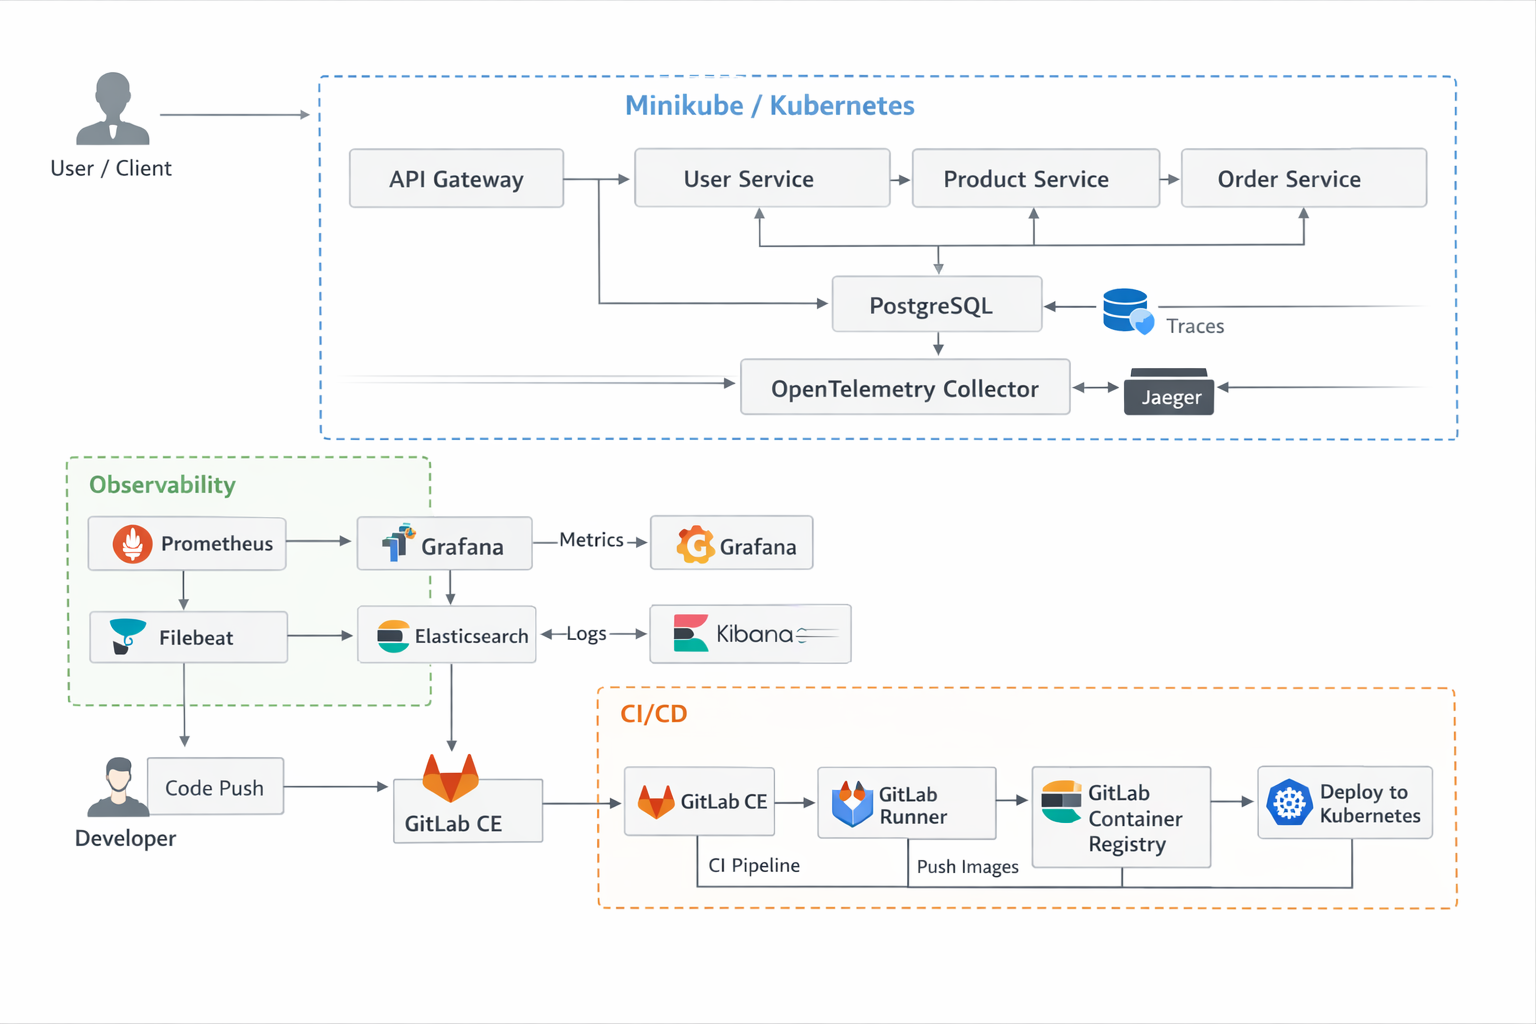
\includegraphics[width=0.96\textwidth]{assets/architecture/lab-overview.png}
\caption{Vista general del laboratorio y relación entre sus bloques principales.}
\label{fig:lab-overview}
\end{figure}

\begin{center}\rule{0.5\linewidth}{0.5pt}\end{center}

\chapter{Objetivos del proyecto}\label{objetivos-del-proyecto}

\section{Objetivo general}\label{objetivo-general}

Diseñar e implementar un laboratorio reproducible de microservicios
observables sobre Kubernetes, incluyendo despliegue, persistencia,
métricas, trazas, logs, alertado y una cadena CI/CD completa con GitLab
self-managed.

\section{Objetivos específicos}\label{objetivos-especuxedficos}

\begin{itemize}
\tightlist
\item
  Construir una base de microservicios Spring Boot con dependencias
  reales entre servicios.
\item
  Desplegar la aplicación sobre Minikube mediante Helm.
\item
  Sustituir datos en memoria por persistencia real con PostgreSQL y
  migraciones con Flyway.
\item
  Instrumentar los servicios con Spring Boot Actuator, Micrometer y
  OpenTelemetry.
\item
  Centralizar métricas en Prometheus y visualizarlas en Grafana.
\item
  Centralizar trazas distribuidas en Jaeger.
\item
  Centralizar logs en Elasticsearch y consultarlos en Kibana.
\item
  Estructurar los logs de aplicación en formato ECS JSON para facilitar
  búsquedas y correlación.
\item
  Definir alertas de observabilidad tanto por métricas como por logs.
\item
  Desplegar GitLab self-managed en el mismo laboratorio.
\item
  Ejecutar pipelines en Kubernetes con GitLab Runner.
\item
  Construir imágenes de contenedor, publicarlas en el GitLab Container
  Registry y desplegarlas por SHA de commit.
\end{itemize}

\begin{center}\rule{0.5\linewidth}{0.5pt}\end{center}

\chapter{Alcance y límites del
laboratorio}\label{alcance-y-luxedmites-del-laboratorio}

Este laboratorio cubre una porción importante del ciclo de vida
operativo de un backend moderno, pero mantiene un alcance
deliberadamente contenido para seguir siendo comprensible y ejecutable
en un entorno local.

\section{Alcance funcional}\label{alcance-funcional}

\begin{itemize}
\tightlist
\item
  cuatro microservicios de negocio
\item
  una librería compartida
\item
  una base de datos PostgreSQL
\item
  despliegue en un único clúster Minikube
\item
  stack de observabilidad completo
\item
  GitLab local con Runner y Registry
\end{itemize}

\section{Límites conscientes}\label{luxedmites-conscientes}

\begin{itemize}
\tightlist
\item
  no se ha buscado alta disponibilidad real
\item
  no se han introducido méltiples clústeres ni méltiples entornos
  completos
\item
  el storage y algunos componentes del chart de GitLab son vélidos para
  laboratorio, no para producción
\item
  algunas decisiones de RBAC y seguridad se han simplificado por ser un
  entorno docente
\end{itemize}

Este enfoque es intencionado. El objetivo no es replicar una plataforma
corporativa en toda su complejidad, sino construir un sistema
suficientemente realista como para aprender de él y explicarlo con
criterio.

\begin{center}\rule{0.5\linewidth}{0.5pt}\end{center}

\chapter{Arquitectura general del
laboratorio}\label{arquitectura-general-del-laboratorio}

La arquitectura final del proyecto puede entenderse como la
superposición de cuatro capas:

\begin{enumerate}
\def\labelenumi{\arabic{enumi}.}
\tightlist
\item
  capa de aplicación\\
\item
  capa de datos\\
\item
  capa de observabilidad\\
\item
  capa de CI/CD y plataforma
\end{enumerate}

\begin{figure}[H]
\centering
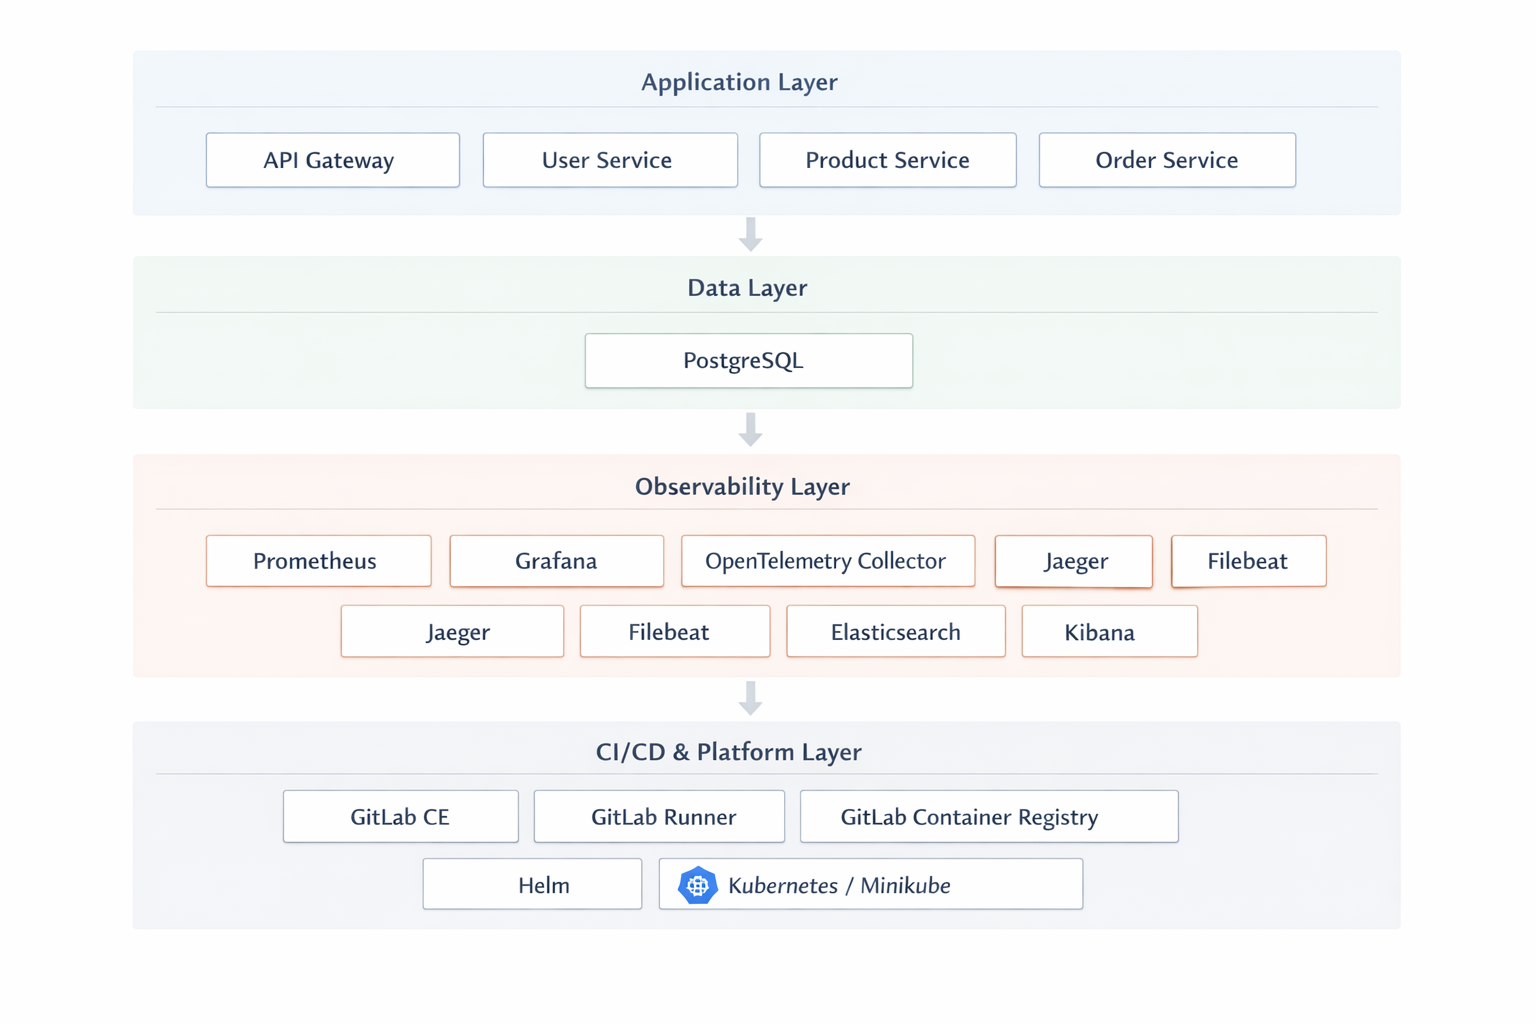
\includegraphics[width=0.96\textwidth]{assets/architecture/layered-architecture.png}
\caption{Arquitectura lógica del laboratorio dividida en cuatro capas.}
\label{fig:layered-architecture}
\end{figure}

\section{Capa de aplicación}\label{capa-de-aplicaciuxf3n}

La aplicación está formada por los siguientes módulos:

\begin{itemize}
\tightlist
\item
  \texttt{api-gateway}
\item
  \texttt{user-service}
\item
  \texttt{product-service}
\item
  \texttt{order-service}
\item
  \texttt{essentials-lib}
\end{itemize}

El flujo principal de negocio es:

\begin{PlainCode}
Cliente -> api-gateway -> order-service -> user-service / product-service
\end{PlainCode}

Este flujo se eligió porque permite demostrar una cadena distribuida
sencilla pero suficiente para practicar:

\begin{itemize}
\tightlist
\item
  trazabilidad entre servicios
\item
  correlación de logs
\item
  métricas por componente
\item
  detección de fallos downstream
\end{itemize}

\section{Capa de datos}\label{capa-de-datos}

La persistencia se resuelve con una instancia PostgreSQL desplegada en
Kubernetes. Cada servicio trabaja sobre su propio esquema, mientras que
las migraciones se controlan de forma independiente con Flyway.

\section{Capa de observabilidad}\label{capa-de-observabilidad}

La observabilidad se compone de:

\begin{itemize}
\tightlist
\item
  Prometheus para métricas
\item
  Grafana para dashboards y alertas de métricas
\item
  OpenTelemetry Collector como agregador de telemetría
\item
  Jaeger para trazas distribuidas
\item
  Filebeat para recolección de logs
\item
  Elasticsearch para almacenamiento y consulta de logs
\item
  Kibana para exploración y alertado basado en logs
\end{itemize}

\section{Capa de CI/CD y
plataforma}\label{capa-de-cicd-y-plataforma}

La automatización de plataforma se apoya en:

\begin{itemize}
\tightlist
\item
  GitLab CE desplegado dentro de Minikube
\item
  GitLab Runner desplegado dentro de Kubernetes
\item
  GitLab Container Registry como registro privado de imágenes
\item
  pipeline GitLab CI para build, test, package, validación Helm, build
  de imágenes y despliegue manual
\end{itemize}

\begin{center}\rule{0.5\linewidth}{0.5pt}\end{center}

\chapter{Estructura del
repositorio}\label{estructura-del-repositorio}

La raíz del repositorio contiene los elementos principales del
laboratorio:

\begin{PlainCode}
.
|-- api-gateway
|-- user-service
|-- product-service
|-- order-service
|-- essentials-lib
|-- deploy
|-- scripts
|-- docs
|-- .gitlab-ci.yml
|-- pom.xml
`-- roadmap.md
\end{PlainCode}

\section{Módulos Maven}\label{muxf3dulos-maven}

El proyecto se construye como multi-módulo Maven. Los módulos de
aplicación comparten dependencias y errores comunes a través de
\texttt{essentials-lib}.

\section{\texorpdfstring{Directorio
\texttt{deploy}}{Directorio deploy}}\label{directorio-deploy}

\texttt{deploy/} concentra la infraestructura declarativa del
laboratorio:

\begin{itemize}
\tightlist
\item
  \texttt{deploy/helm} para charts de aplicación y PostgreSQL
\item
  \texttt{deploy/environments/minikube} para valores del entorno local
\item
  \texttt{deploy/observability} para Prometheus, Grafana, Jaeger, OTel
  Collector y stack Elastic
\item
  \texttt{deploy/gitlab} para la instalación de GitLab
\item
  \texttt{deploy/gitlab-runner} para la instalación del runner y sus
  permisos
\end{itemize}

\section{\texorpdfstring{Directorio
\texttt{scripts}}{Directorio scripts}}\label{directorio-scripts}

El directorio \texttt{scripts/} contiene automatizaciones prácticas
para:

\begin{itemize}
\tightlist
\item
  construir imágenes locales o para Minikube
\item
  desplegar aplicación
\item
  desplegar observabilidad
\item
  instalar ECK
\item
  abrir y cerrar port-forwards
\item
  validar endpoints
\end{itemize}

Esta capa de scripts es muy importante desde el punto de vista
didáctico, porque muestra cómo convertir pasos manuales en operaciones
repetibles.

\begin{center}\rule{0.5\linewidth}{0.5pt}\end{center}

\chapter{Construcción de la base de
microservicios}\label{construcciuxf3n-de-la-base-de-microservicios}

\section{Diseño inicial}\label{diseuxf1o-inicial}

La primera fase del proyecto consistió en construir una base mínima
sobre la que luego poder introducir observabilidad y automatización. Se
definieron cuatro servicios:

\begin{itemize}
\tightlist
\item
  \texttt{user-service}: catálogo de usuarios
\item
  \texttt{product-service}: catálogo de productos
\item
  \texttt{order-service}: gestión de pedidos y dependencia de los
  catálogos
\item
  \texttt{api-gateway}: punto de entrada unificado
\end{itemize}

Este diseño responde a una idea pedagógica clara: si los servicios son
completamente independientes, la observabilidad distribuida pierde
valor. En cambio, al introducir una cadena de dependencias, el proyecto
gana interés real.

\section{Evolución hacia una estructura más
mantenible}\label{evoluciuxf3n-hacia-una-estructura-muxe1s-mantenible}

Conforme el proyecto creció, los servicios evolucionaron hacia una
estructura por capas:

\begin{itemize}
\tightlist
\item
  \texttt{api}
\item
  \texttt{service}
\item
  \texttt{service/impl}
\item
  \texttt{repository}
\item
  \texttt{model}
\end{itemize}

También se introdujeron:

\begin{itemize}
\tightlist
\item
  DTOs generados a partir de OpenAPI
\item
  interfaces de servicio
\item
  separación entre lógica de negocio y acceso a datos
\item
  manejo común de errores desde la librería compartida
\end{itemize}

Desde el punto de vista de ingeniería, esto es importante porque evita
que la base del laboratorio se convierta en una demo frágil. Una
plataforma de observabilidad se beneficia de una aplicación
razonablemente estructurada.

\section{Ejemplo de responsabilidad en el
gateway}\label{ejemplo-de-responsabilidad-en-el-gateway}

El gateway no es un simple proxy ciego, sino un componente que
centraliza acceso y facilita el seguimiento del flujo completo:

\begin{JavaCode}
public interface GatewayService {
    Object getOverview();
    Object getUsers();
    Object getProducts();
    Object getOrders();
}
\end{JavaCode}

Este tipo de interfaz permite:

\begin{itemize}
\tightlist
\item
  encapsular llamadas downstream
\item
  instrumentar mejor el flujo
\item
  registrar logs útiles
\item
  centralizar puntos de fallo y latencia
\end{itemize}

\section{Qué hace exactamente cada
módulo}\label{quuxe9-hace-exactamente-cada-muxf3dulo}

Una forma muy útil de entender el proyecto es separar responsabilidades
por módulo. La siguiente tabla resume la función de cada uno y por qué
existe.

{\def\LTcaptype{none} % do not increment counter
\begin{longtable}[]{@{}
  >{\raggedright\arraybackslash}p{(\linewidth - 6\tabcolsep) * \real{0.2500}}
  >{\raggedright\arraybackslash}p{(\linewidth - 6\tabcolsep) * \real{0.2500}}
  >{\raggedright\arraybackslash}p{(\linewidth - 6\tabcolsep) * \real{0.2500}}
  >{\raggedright\arraybackslash}p{(\linewidth - 6\tabcolsep) * \real{0.2500}}@{}}
\toprule\noalign{}
\begin{minipage}[b]{\linewidth}\raggedright
Módulo
\end{minipage} & \begin{minipage}[b]{\linewidth}\raggedright
Responsabilidad principal
\end{minipage} & \begin{minipage}[b]{\linewidth}\raggedright
Tecnologías destacadas
\end{minipage} & \begin{minipage}[b]{\linewidth}\raggedright
Por qué es importante
\end{minipage} \\
\midrule\noalign{}
\endhead
\bottomrule\noalign{}
\endlastfoot
\texttt{api-gateway} & Punto de entrada unificado & Spring Web,
Actuator, Prometheus, OTel, ECS logging & Permite observar llamadas
agregadas y errores downstream \\
\texttt{user-service} & Gestión de usuarios & Spring Web, JPA, Flyway,
PostgreSQL & Introduce persistencia y validaciones de negocio \\
\texttt{product-service} & Gestión de productos & Spring Web, JPA,
Flyway, PostgreSQL & Aporta catálogo persistente y otro dominio de
negocio \\
\texttt{order-service} & Gestión de pedidos y orquestación & Spring Web,
JPA, Flyway, RestClient, OTel \texttt{@WithSpan} & Es el mejor punto
para enseñar trazas distribuidas \\
\texttt{essentials-lib} & Código común & Excepciones comunes, manejo de
errores & Evita duplicación y unifica respuesta de errores \\
\end{longtable}
}

\section{Por qué se eligió este flujo de
negocio}\label{por-quuxe9-se-eligiuxf3-este-flujo-de-negocio}

El flujo
\texttt{gateway\ -\textgreater{}\ order-service\ -\textgreater{}\ user-service/product-service}
no es arbitrario. Desde un punto de vista docente, es ideal porque reúne
varios escenarios frecuentes:

\begin{itemize}
\tightlist
\item
  un servicio frontal que recibe tráfico del cliente
\item
  un servicio de negocio que agrega información
\item
  dos servicios de catálogo consultados en tiempo de ejecución
\item
  puntos claros donde medir latencia
\item
  puntos claros donde registrar fallos downstream
\item
  contexto suficiente para generar trazas distribuidas interesantes
\end{itemize}

Si todos los servicios fueran completamente autónomos, la parte de
observabilidad distribuida sería menos expresiva. En cambio, con esta
topología se puede responder a preguntas como:

\begin{itemize}
\tightlist
\item
  ¿cuánto tarda una petición completa?
\item
  ¿qué servicio fue el más lento?
\item
  ¿falló el servicio frontal o un servicio dependiente?
\item
  ¿hay logs de error asociados al mismo \texttt{trace\_id}?
\end{itemize}

\section{Ejemplo real de llamada downstream en el
gateway}\label{ejemplo-real-de-llamada-downstream-en-el-gateway}

El siguiente fragmento del gateway resume muy bien la filosofía del
proyecto: hacer visibles las llamadas entre servicios y tratarlas como
parte del sistema observable, no como una caja negra.

\begin{JavaCode}
private ResponseEntity<Object> forwardGet(String baseUrl, String path, Object... uriVariables) {
    String target = baseUrl + path;
    try {
        log.info("Forwarding GET request to {}", target);
        Object body = restClient.get()
                .uri(target, uriVariables)
                .retrieve()
                .body(Object.class);
        log.info("GET {} completed successfully", target);
        return ResponseEntity.ok(body);
    } catch (RestClientResponseException exception) {
        log.warn("GET {} returned downstream status {}", target, exception.getStatusCode().value());
        return buildDownstreamResponse(exception);
    } catch (RestClientException exception) {
        log.error("GET {} failed because downstream is unavailable", target, exception);
        return buildUnavailableResponse(exception);
    }
}
\end{JavaCode}

\section{Qué enseña este
fragmento}\label{quuxe9-enseuxf1a-este-fragmento}

\begin{itemize}
\tightlist
\item
  \texttt{RestClient} encapsula la llamada HTTP al siguiente servicio.
\item
  \texttt{log.info} permite seguir el camino feliz del flujo.
\item
  \texttt{log.warn} captura respuestas erróneas del servicio downstream.
\item
  \texttt{log.error} captura indisponibilidad real del downstream.
\item
  la respuesta al cliente se construye de forma explícita, evitando
  excepciones opacas.
\end{itemize}

Desde el punto de vista de observabilidad, este código es valioso porque
produce:

\begin{itemize}
\tightlist
\item
  métricas HTTP en el servicio
\item
  logs semánticamente útiles
\item
  trazas que se pueden seguir en Jaeger
\end{itemize}

\begin{center}\rule{0.5\linewidth}{0.5pt}\end{center}

\chapter{Persistencia real con PostgreSQL y
Flyway}\label{persistencia-real-con-postgresql-y-flyway}

\section{De datos en memoria a
persistencia}\label{de-datos-en-memoria-a-persistencia}

Uno de los primeros saltos de madurez del proyecto fue abandonar el
modelo puramente en memoria. Esto permitió acercar el laboratorio a un
escenario mucho más realista, donde existen migraciones, estado
persistente y problemas de compatibilidad entre entornos.

\section{Despliegue de PostgreSQL en
Kubernetes}\label{despliegue-de-postgresql-en-kubernetes}

Se creó un chart Helm propio para PostgreSQL, con plantillas para:

\begin{itemize}
\tightlist
\item
  \texttt{Deployment}
\item
  \texttt{Service}
\item
  \texttt{Secret}
\item
  \texttt{PersistentVolumeClaim}
\end{itemize}

La presencia del \texttt{PersistentVolumeClaim} es clave porque
garantiza continuidad del estado entre reinicios del pod.

\section{Migraciones con Flyway}\label{migraciones-con-flyway}

Cada servicio gestiona sus migraciones de forma independiente. El
enfoque seguido fue:

\begin{itemize}
\tightlist
\item
  una única instancia PostgreSQL
\item
  un esquema por microservicio
\item
  Flyway como mecanismo de versionado de base de datos
\end{itemize}

Este diseño es simple y útil para laboratorio, porque permite practicar
versionado de esquema sin multiplicar el número de bases.

\section{Problemas reales con
migraciones}\label{problemas-reales-con-migraciones}

Durante el desarrollo aparecieron problemas clásicos de evolución de
base de datos:

\begin{itemize}
\tightlist
\item
  modificación de migraciones ya aplicadas
\item
  divergencia entre historial y estado real
\item
  necesidad de reparar el historial de Flyway
\end{itemize}

Este punto tiene mucho valor pedagógico, porque enseña una lección
fundamental: las migraciones no son un detalle accesorio, forman parte
del contrato operativo del sistema.

\section{Tests con Testcontainers}\label{tests-con-testcontainers}

Para evitar falsos positivos asociados a H2, las pruebas se alinearon
más con el entorno real usando PostgreSQL efímero con Testcontainers. La
ventaja principal es que el comportamiento de base de datos se acerca
mucho más al de producción o preproducción.

\section{Qué problema resuelve Flyway en este
laboratorio}\label{quuxe9-problema-resuelve-flyway-en-este-laboratorio}

Cuando un proyecto usa JPA y una base de datos relacional, existe una
tentación frecuente: dejar que Hibernate cree o altere el esquema
automáticamente. Para un laboratorio pequeño puede parecer suficiente,
pero tiene varias desventajas:

\begin{itemize}
\tightlist
\item
  no queda versión explícita del esquema
\item
  no hay trazabilidad de cambios
\item
  es difícil reproducir estados históricos
\item
  aparecen diferencias entre entornos
\end{itemize}

Por eso aquí se eligió:

\begin{itemize}
\tightlist
\item
  \texttt{spring.jpa.hibernate.ddl-auto=validate}
\item
  Flyway como responsable único de crear y evolucionar el esquema
\end{itemize}

Ese diseño separa claramente dos responsabilidades:

{\def\LTcaptype{none} % do not increment counter
\begin{longtable}[]{@{}ll@{}}
\toprule\noalign{}
Herramienta & Responsabilidad \\
\midrule\noalign{}
\endhead
\bottomrule\noalign{}
\endlastfoot
Hibernate / JPA & Validar que el modelo Java encaja con el esquema \\
Flyway & Crear y versionar el esquema real \\
\end{longtable}
}

\section{Ejemplo real de configuración de base de
datos}\label{ejemplo-real-de-configuraciuxf3n-de-base-de-datos}

En \texttt{user-service} la configuración principal quedó así:

\begin{PropertiesCode}
spring.datasource.url=${SPRING_DATASOURCE_URL:jdbc:postgresql://localhost:5432/ecommerce_platform}
spring.datasource.username=${SPRING_DATASOURCE_USERNAME:ecommerce}
spring.datasource.password=${SPRING_DATASOURCE_PASSWORD:ecommerce123}
spring.jpa.hibernate.ddl-auto=validate
spring.jpa.open-in-view=false
spring.jpa.properties.hibernate.default_schema=user_service
spring.flyway.create-schemas=true
spring.flyway.schemas=user_service
\end{PropertiesCode}


\section{Explicación línea a
línea}\label{explicaciuxf3n-luxednea-a-luxednea}

\begin{itemize}
\tightlist
\item
  \texttt{spring.datasource.url}: define el endpoint de PostgreSQL.
\item
  \texttt{username} y \texttt{password}: desacoplan credenciales del
  código.
\item
  \texttt{ddl-auto=validate}: obliga a que el esquema exista y sea
  compatible.
\item
  \texttt{open-in-view=false}: evita extender el contexto de
  persistencia hasta la capa web.
\item
  \texttt{default\_schema=user\_service}: separa el dominio de usuario
  del resto.
\item
  \texttt{flyway.create-schemas=true}: permite que Flyway cree el
  esquema si no existe.
\item
  \texttt{flyway.schemas} y \texttt{flyway.default-schema}: limitan la
  migración al esquema del servicio.
\end{itemize}

\section{Por qué se usaron esquemas
separados}\label{por-quuxe9-se-usaron-esquemas-separados}

En vez de levantar cuatro bases de datos distintas, el proyecto usa una
sola instancia PostgreSQL con varios esquemas. Esto tiene ventajas
claras para un laboratorio:

\begin{itemize}
\tightlist
\item
  menos componentes que operar
\item
  menos consumo de recursos
\item
  mismo motor y mismas credenciales base
\item
  aislamiento lógico razonable entre dominios
\end{itemize}

Es un compromiso didáctico muy útil. Permite enseñar separación de
dominios sin convertir el laboratorio en una instalación de base de
datos excesivamente pesada.

\section{Testcontainers en la
práctica}\label{testcontainers-en-la-pruxe1ctica}

La configuración de test de \texttt{user-service} muestra muy bien la
idea:

\begin{PropertiesCode}
spring.datasource.url=jdbc:tc:postgresql:16-alpine:///userdb
spring.datasource.driver-class-name=org.testcontainers.jdbc.ContainerDatabaseDriver
spring.datasource.username=test
spring.datasource.password=test
spring.jpa.hibernate.ddl-auto=validate
spring.jpa.properties.hibernate.default_schema=user_service
spring.flyway.create-schemas=true
spring.flyway.schemas=user_service
spring.flyway.default-schema=user_service
otel.sdk.disabled=true
\end{PropertiesCode}

\section{Qué enseña esta configuración de
test}\label{quuxe9-enseuxf1a-esta-configuraciuxf3n-de-test}

\begin{itemize}
\tightlist
\item
  \texttt{jdbc:tc:postgresql:16-alpine:///userdb} hace que
  Testcontainers levante PostgreSQL automáticamente.
\item
  el driver \texttt{ContainerDatabaseDriver} abstrae el arranque del
  contenedor.
\item
  el test sigue validando esquema y migraciones reales.
\item
  \texttt{otel.sdk.disabled=true} evita ruido de telemetría en tests de
  contexto.
\end{itemize}

Este detalle es importante para la memoria: explica por qué la pipeline
necesita acceso a Docker en la fase de tests.

\section{Evidencia de los microservicios y de la base de datos}\label{evidencia-de-los-microservicios-y-de-la-base-de-datos}

\begin{BashCode}
kubectl get pods -n default
NAME                               READY   STATUS    RESTARTS        AGE
api-gateway-7c68cdbfbb-vj55l       1/1     Running   1 (28m ago)     17h
order-service-6858fb5df6-nwqvc     1/1     Running   0               4m20s
postgres-67c4c56db5-gxm6x          1/1     Running   7 (3m45s ago)   47h
product-service-7f5bd75f96-htrlj   1/1     Running   2 (2m39s ago)   5m2s
user-service-66cc6c69b6-knwgf      1/1     Running   1 (2m48s ago)   5m2s
\end{BashCode}

Esta salida ilustra bien el objetivo de la sección porque deja ver, de
forma inmediata, que PostgreSQL y los cuatro microservicios se
encuentran operativos y listos para recibir tráfico dentro del
namespace \texttt{default}.

\begin{center}\rule{0.5\linewidth}{0.5pt}\end{center}

\chapter{Despliegue en Kubernetes con
Helm}\label{despliegue-en-kubernetes-con-helm}

\section{Qué es Kubernetes y qué problema
resuelve}\label{quuxe9-es-kubernetes-y-quuxe9-problema-resuelve}

Kubernetes es una plataforma de orquestación de contenedores diseñada
para ejecutar aplicaciones distribuidas de forma declarativa. La idea
clave no es lanzar procesos manualmente, sino describir cuál debe ser el
estado deseado del sistema y dejar que la plataforma trabaje de manera
continua para mantener ese estado. En vez de pedirle al operador que
arranque un contenedor concreto, abra un puerto y vigile reinicios,
Kubernetes permite declarar que una aplicación debe tener una o varias
réplicas, que debe exponerse mediante un servicio de red y que debe
reiniciarse automáticamente si deja de responder.

En términos prácticos, Kubernetes resuelve varios problemas muy comunes
cuando una aplicación deja de ser un proceso local y pasa a ejecutarse
como sistema distribuido:

\begin{itemize}
\tightlist
\item
  planificación de contenedores sobre nodos disponibles
\item
  reinicio automático cuando un proceso falla
\item
  descubrimiento de servicios dentro del clúster
\item
  balanceo de tráfico entre réplicas
\item
  separación entre configuración, secretos y binario
\item
  despliegues repetibles y trazables
\end{itemize}

El modelo mental más importante es entender que
Kubernetes trabaja como un sistema de reconciliación. El usuario declara
una intención, por ejemplo: ``quiero un \texttt{Deployment} con una
réplica de \texttt{user-service} escuchando en el puerto 8080''. A
partir de ahí, el plano de control compara continuamente el estado real
con el estado deseado. Si el pod muere, Kubernetes crea otro. Si el nodo
se reinicia, la plataforma vuelve a programar la carga. Si la aplicación
no responde a las sondas, el pod deja de considerarse disponible.

\section{Conceptos básicos para entender un
despliegue}\label{conceptos-buxe1sicos-para-entender-un-despliegue}

Antes de leer los charts de Helm conviene dominar los objetos mínimos
que intervienen en este laboratorio:

\begin{itemize}
\tightlist
\item
  \textbf{Pod}. Es la unidad mínima de ejecución en Kubernetes. En este
  proyecto cada microservicio corre dentro de un pod gestionado por un
  \texttt{Deployment}. Un pod no se trata como una máquina virtual, sino
  como un envoltorio efímero que puede destruirse y recrearse.
\item
  \textbf{Deployment}. Define cómo debe ejecutarse un conjunto de pods
  equivalentes. Permite decir cuántas réplicas debe haber, qué imagen se
  ejecuta y cómo se actualiza una versión por otra.
\item
  \textbf{Service}. Da una identidad de red estable a un conjunto de
  pods. En este laboratorio los microservicios internos usan
  \texttt{ClusterIP} y el \texttt{api-gateway} se publica como
  \texttt{NodePort} para aceptar tráfico desde fuera del clúster.
\item
  \textbf{ConfigMap y Secret}. Separan la configuración del contenedor.
  Gracias a eso, una imagen puede moverse entre entornos sin ser
  reconstruida solo por cambiar una URL o una credencial.
\item
  \textbf{Probe}. Las sondas de \texttt{startup}, \texttt{readiness} y
  \texttt{liveness} permiten a Kubernetes decidir si la aplicación ya ha
  terminado de arrancar, si está preparada para recibir tráfico y si
  debe reiniciarse.
\item
  \textbf{PersistentVolumeClaim}. En PostgreSQL se usa para no perder
  datos al reiniciar el pod de base de datos.
\end{itemize}

Un ejemplo muy simple ayuda a fijar la idea. Si un \texttt{Deployment}
de \texttt{user-service} declara una réplica y una imagen concreta,
Kubernetes intentará mantener siempre exactamente un pod de ese servicio.
Si además existe un \texttt{Service} llamado \texttt{user-service}, el
resto de aplicaciones del clúster no tienen que conocer la IP cambiante
del pod, sino solo el nombre DNS estable del servicio.

\section{Cómo funciona Kubernetes dentro de este
laboratorio}\label{cuxf3mo-funciona-kubernetes-dentro-de-este-laboratorio}

En este proyecto Kubernetes se ejecuta sobre Minikube, lo que permite
simular un entorno de plataforma completo dentro de un portátil. Aunque
se trata de un laboratorio local, los conceptos operativos son los
mismos que aparecerían en un entorno real:

\begin{itemize}
\tightlist
\item
  Minikube actúa como clúster de Kubernetes.
\item
  Los microservicios y PostgreSQL se despliegan en el namespace
  \texttt{default}.
\item
  GitLab y GitLab Runner se ejecutan también dentro del clúster, aunque
  en namespaces separados.
\item
  La pila de observabilidad convive con la aplicación y consume métricas,
  logs y trazas de los pods.
\end{itemize}

Esto hace que el laboratorio sea especialmente didáctico, porque permite
observar cómo se relacionan los componentes de aplicación con los de
plataforma. Por ejemplo, cuando un pod no queda \texttt{Ready}, no basta
con ver el log de Spring Boot: también hay que revisar sondas,
\texttt{Services}, eventos del scheduler y estado del rollout.
Kubernetes obliga a pensar la aplicación como parte de un sistema más
amplio.

\section{Qué aporta Helm por encima de
\texttt{kubectl apply}}\label{quuxe9-aporta-helm-por-encima-de-kubectl-apply}

\texttt{kubectl apply} permite crear recursos Kubernetes a partir de
manifiestos YAML estáticos. Es suficiente para ejemplos sencillos, pero
se queda corto cuando el número de servicios crece y aparecen
variaciones entre entornos. Helm añade una capa de empaquetado,
templating y versionado sobre esos manifiestos.

En otras palabras, Helm permite tratar un conjunto de recursos
Kubernetes como una unidad desplegable. Un \emph{chart} agrupa
\texttt{Deployment}, \texttt{Service}, \texttt{ConfigMap},
\texttt{Secret} y cualquier otro recurso asociado a un componente. Los
valores variables se extraen a ficheros \texttt{values.yaml}, lo que
facilita reutilizar la misma plantilla en varios entornos cambiando solo
parámetros concretos.

En este laboratorio Helm aporta tres ventajas clave:

\begin{itemize}
\tightlist
\item
  evita duplicar manifiestos casi idénticos entre microservicios y
  entornos
\item
  permite inyectar parámetros como imagen, tag, probes y recursos de red
  sin reescribir las plantillas base
\item
  hace posible usar \texttt{helm upgrade --install} para tener un flujo
  de despliegue idempotente y fácil de automatizar desde CI/CD
\end{itemize}

\section{Motivación para usar
Helm}\label{motivaciuxf3n-para-usar-helm}

Una vez que la aplicación dejó de ser local y pasí a ejecutarse en
Kubernetes, era necesario un mecanismo para empaquetar recursos,
parametrizarlos y reutilizarlos por entorno. Helm cubre exactamente esa
necesidad.

\section{Un chart por servicio}\label{un-chart-por-servicio}

Cada microservicio dispone de su propio chart:

\begin{itemize}
\tightlist
\item
  \texttt{deploy/helm/api-gateway}
\item
  \texttt{deploy/helm/user-service}
\item
  \texttt{deploy/helm/product-service}
\item
  \texttt{deploy/helm/order-service}
\item
  \texttt{deploy/helm/postgres}
\end{itemize}

Este enfoque facilita:

\begin{itemize}
\tightlist
\item
  despliegues independientes
\item
  configuración específica por servicio
\item
  evolución aislada de recursos Kubernetes
\end{itemize}

\section{Separación entre chart y
entorno}\label{separaciuxf3n-entre-chart-y-entorno}

Los charts contienen valores por defecto, mientras que el entorno
Minikube se parametriza en:

\begin{itemize}
\tightlist
\item
  \texttt{deploy/environments/minikube/api-gateway-values.yaml}
\item
  \texttt{deploy/environments/minikube/user-service-values.yaml}
\item
  \texttt{deploy/environments/minikube/product-service-values.yaml}
\item
  \texttt{deploy/environments/minikube/order-service-values.yaml}
\item
  \texttt{deploy/environments/minikube/postgres-values.yaml}
\end{itemize}

Esta separación es muy útil porque evita duplicar charts y permite
adaptar comportamiento por entorno sin modificar plantillas.

\section{Automatización del
despliegue}\label{automatizaciuxf3n-del-despliegue}

El laboratorio incluye scripts específicos como:

\begin{itemize}
\tightlist
\item
  \texttt{scripts/build-minikube-images.ps1}
\item
  \texttt{scripts/deploy-minikube.ps1}
\end{itemize}

El primero sirve para construir imágenes directamente dentro de
Minikube. El segundo empaqueta el despliegue completo con Helm y espera
a que los rollouts terminen correctamente.

\section{Aprendizaje principal}\label{aprendizaje-principal}

Kubernetes no debe entenderse solo como ``levantar pods''. La operación
real exige:

\begin{itemize}
\tightlist
\item
  empaquetado
\item
  parámetros por entorno
\item
  restart controlado
\item
  espera de readiness
\item
  diagnóstico cuando un rollout falla
\end{itemize}

\section{Anatomía de un chart Helm de
microservicio}\label{anatomuxeda-de-un-chart-helm-de-microservicio}

El chart de \texttt{api-gateway} es suficientemente simple como para
explicarlo casi línea a línea. Su \texttt{values.yaml} contiene:

\begin{YamlCode}
replicaCount: 1

image:
  repository: mercadona/api-gateway
  tag: 0.0.1-SNAPSHOT
  pullPolicy: IfNotPresent
  pullSecrets: []

containerPort: 8080

service:
  type: ClusterIP
  port: 8080
  targetPort: 8080
  nodePort: null
\end{YamlCode}

\section{\texorpdfstring{Qué enseña este
\texttt{values.yaml}}{8.7 Qué enseña este values.yaml}}\label{quuxe9-enseuxf1a-este-values.yaml}

\begin{itemize}
\tightlist
\item
  \texttt{replicaCount}: número deseado de pods.
\item
  \texttt{image.repository}: de dónde sale la imagen.
\item
  \texttt{image.tag}: qué versión concreta se quiere ejecutar.
\item
  \texttt{pullPolicy}: cuándo debe descargar la imagen.
\item
  \texttt{pullSecrets}: credenciales para un registry privado.
\item
  \texttt{service.type}: cómo se expondrá el servicio.
\end{itemize}

Este fichero es muy útil en una memoria docente porque muestra que Helm
no ``crea magia'', sino que parametriza decisiones de despliegue
explícitas.

\section{Plantilla real del
Deployment}\label{plantilla-real-del-deployment}

El \texttt{deployment.yaml} del chart de \texttt{api-gateway} quedó así:

\begin{YamlCode}
apiVersion: apps/v1
kind: Deployment
metadata:
  name: {{ .Chart.Name }}
spec:
  replicas: {{ .Values.replicaCount }}
  template:
    spec:
      {{- with .Values.image.pullSecrets }}
      imagePullSecrets:
{{ toYaml . | indent 8 }}
      {{- end }}
      containers:
        - name: {{ .Chart.Name }}
          image: "{{ .Values.image.repository }}:{{ .Values.image.tag }}"
          imagePullPolicy: {{ .Values.image.pullPolicy }}
\end{YamlCode}

\section{Cómo leer esta plantilla}\label{cuxf3mo-leer-esta-plantilla}

\begin{itemize}
\tightlist
\item
  \texttt{\{\{\ .Chart.Name\ \}\}}: usa el nombre del chart como nombre
  del deployment y del contenedor.
\item
  \texttt{\{\{\ .Values.*\ \}\}}: inyecta valores desde
  \texttt{values.yaml} o desde un fichero de entorno.
\item
  \texttt{with\ .Values.image.pullSecrets}: añade
  \texttt{imagePullSecrets} solo si hay credenciales definidas.
\item
  \texttt{image.repository} y \texttt{image.tag}: permiten separar la
  plantilla del detalle de versión.
\end{itemize}

La gran enseñanza aquí es que Helm no reemplaza Kubernetes. Helm es una
capa de parametrización y reutilización sobre Kubernetes.

\section{Valores específicos de
Minikube}\label{valores-especuxedficos-de-minikube}

El entorno de Minikube modifica el comportamiento del chart. Por
ejemplo, \texttt{api-gateway-values.yaml} contiene:

\begin{YamlCode}
image:
  pullPolicy: IfNotPresent
  pullSecrets:
    - name: gitlab-registry-creds

service:
  type: NodePort
  nodePort: 30080

env:
  - name: USER_SERVICE_URL
    value: http://user-service:8080
\end{YamlCode}

\section{Qué problema resuelve esta capa de
values}\label{quuxe9-problema-resuelve-esta-capa-de-values}

Sin un fichero por entorno, el chart tendría que codificar detalles del
laboratorio:

\begin{itemize}
\tightlist
\item
  \texttt{NodePort}
\item
  nombres de servicios internos
\item
  credenciales de registry
\item
  URLs de servicios downstream
\end{itemize}

Ese sería un diseño pobre, porque mezclaría plantilla base con detalles
del entorno. Separarlo mejora mucho la mantenibilidad.

\section{Script de despliegue y lógica
operativa}\label{script-de-despliegue-y-luxf3gica-operativa}

El script \texttt{deploy-minikube.ps1} es un buen ejemplo de
automatización incremental. No se limita a aplicar YAML, sino que
incorpora diagnóstico.

Fragmento representativo:

\begin{PowerShellCode}
function Wait-DeploymentRollout {
    param(
        [string]$Name,
        [int]$TimeoutSeconds = 180
    )

    $result = kubectl rollout status deployment/$Name --timeout="$($TimeoutSeconds)s" 2>&1
    if ($LASTEXITCODE -eq 0) {
        $result | Write-Host
        return
    }

    kubectl describe deployment $Name
    kubectl get pods -l app=$Name -o wide
    kubectl logs deployment/$Name --tail=120 --all-containers=true
    throw "Rollout failed for deployment $Name"
}
\end{PowerShellCode}

\section{Qué enseña este
script}\label{quuxe9-enseuxf1a-este-script}

\begin{itemize}
\tightlist
\item
  espera activa del rollout
\item
  salida rápida cuando todo va bien
\item
  captura de diagnóstico cuando algo falla
\item
  uso de \texttt{describe} y \texttt{logs} como rutina de
  troubleshooting
\end{itemize}

Este patrón es muy valioso porque enseña una disciplina
operativa concreta: automatizar no es solo ejecutar, también es saber
diagnosticar.

\section{Evidencia operativa de servicios
publicados}\label{evidencia-operativa-de-servicios-publicados}

En lugar de dejar esta parte como una figura sugerida, resulta más útil
incluir una evidencia real de cómo Kubernetes expone cada componente.
La siguiente salida permite entender, de forma directa, qué servicios se
publican hacia fuera y cuáles permanecen como red interna del clúster:

\begin{BashCode}
kubectl get svc -n default
NAME              TYPE        CLUSTER-IP      EXTERNAL-IP   PORT(S)          AGE
api-gateway       NodePort    10.110.19.72    <none>        8080:30080/TCP   4d
kubernetes        ClusterIP   10.96.0.1       <none>        443/TCP          4d2h
order-service     ClusterIP   10.110.128.46   <none>        8080/TCP         4d
postgres          ClusterIP   10.110.32.253   <none>        5432/TCP         2d
product-service   ClusterIP   10.97.80.94     <none>        8080/TCP         4d
user-service      ClusterIP   10.108.157.40   <none>        8080/TCP         4d
\end{BashCode}

La lectura de esta tabla es muy formativa para entender el modelo de red
básico de Kubernetes:

\begin{itemize}
\tightlist
\item
  \texttt{api-gateway} aparece como \texttt{NodePort}, lo que significa
  que Kubernetes publica el servicio en un puerto del nodo para aceptar
  tráfico externo.
\item
  \texttt{user-service}, \texttt{product-service},
  \texttt{order-service} y \texttt{postgres} se exponen como
  \texttt{ClusterIP}, por lo que solo son accesibles desde dentro del
  clúster.
\item
  Esta separación refleja una práctica habitual: concentrar el acceso
  externo en un punto de entrada y mantener el resto de componentes como
  servicios internos.
\end{itemize}

Dicho de otra forma, el \texttt{api-gateway} actúa como fachada de la
aplicación, mientras que los demás servicios quedan protegidos detrás de
la red interna de Kubernetes. Esto simplifica el encaminamiento,
centraliza políticas de entrada y evita exponer innecesariamente cada
microservicio hacia el exterior.

\begin{center}\rule{0.5\linewidth}{0.5pt}\end{center}

\chapter{Observabilidad de métricas y
trazas}\label{observabilidad-de-muxe9tricas-y-trazas}

\section{Instrumentación con Actuator y
Micrometer}\label{instrumentaciuxf3n-con-actuator-y-micrometer}

La primera capa de observabilidad se construyó con:

\begin{itemize}
\tightlist
\item
  Spring Boot Actuator
\item
  Micrometer
\item
  exposición del endpoint \texttt{/actuator/prometheus}
\end{itemize}

Con ello, cada servicio pudo empezar a publicar:

\begin{itemize}
\tightlist
\item
  métricas JVM
\item
  métricas HTTP
\item
  información básica de health y readiness
\end{itemize}

\section{OpenTelemetry}\label{opentelemetry}

Para las trazas distribuidas se introdujo OpenTelemetry como estándar de
instrumentación y exportación. Esta decisión cambia de forma notable el
comportamiento de los microservicios: dejan de ser cajas negras que solo
responden con un código HTTP y pasan a emitir información estructurada
sobre qué operación están ejecutando, cuánto tarda cada tramo y cómo se
encadenan las llamadas entre servicios.

En Spring Boot, el \texttt{opentelemetry-spring-boot-starter} añade de
forma automática instrumentación sobre elementos muy habituales del
framework:

\begin{itemize}
\tightlist
\item
  peticiones HTTP entrantes servidas por Spring MVC
\item
  llamadas HTTP salientes realizadas con clientes compatibles
\item
  acceso a base de datos a través de JDBC
\item
  metadatos del servicio, como nombre, entorno y namespace lógico
\end{itemize}

Eso significa que una petición aparentemente simple, como un
\texttt{POST /api/orders}, deja rastros en varios niveles. El gateway
crea un span de entrada, \texttt{order-service} crea spans de negocio y,
además, aparecen spans derivados de las consultas a \texttt{user-service},
\texttt{product-service} y PostgreSQL. La traza final cuenta la historia
completa de la operación.

Otro punto importante es que OpenTelemetry no es solo una librería, sino
un modelo común. Permite describir telemetría con conceptos estándar,
como \texttt{trace}, \texttt{span}, atributos y contexto propagado.
Gracias a eso, Jaeger puede reconstruir una petición completa aunque
haya pasado por varios microservicios diferentes.

Conviene introducir aquí el concepto de \textbf{OTLP}. OTLP significa
\emph{OpenTelemetry Protocol}. Es el protocolo estándar con el que una
aplicación instrumentada envía su telemetría a un collector o backend.
En este proyecto se usa OTLP sobre HTTP/Protobuf, lo que permite que
cada microservicio entregue sus spans al OTel Collector sin depender de
un formato propietario.

\section{OpenTelemetry Collector}\label{opentelemetry-collector}

El OTel Collector se desplegó como componente intermedio para:

\begin{itemize}
\tightlist
\item
  recibir spans
\item
  procesarlos
\item
  redirigirlos a Jaeger
\end{itemize}

Esta pieza es muy didáctica porque introduce la idea de canalizar
telemetría a través de un punto de agregación y no enviar todo
directamente desde la aplicación al backend final.

\section{Jaeger}\label{jaeger}

Jaeger se incorporó para visualizar las trazas distribuidas. Gracias a
ello fue posible:

\begin{itemize}
\tightlist
\item
  seguir una petición entre varios servicios
\item
  detectar llamadas downstream
\item
  validar correlación con logs mediante \texttt{trace\_id}
\end{itemize}

\section{Ejemplo de valor
operativo}\label{ejemplo-de-valor-operativo}

En un laboratorio simple podría parecer suficiente ver tiempos de
respuesta en Grafana. Sin embargo, las trazas aportan una capa distinta:

\begin{itemize}
\tightlist
\item
  qué servicio llamó a cuál
\item
  cuánto tardó cada salto
\item
  dónde fallí una petición concreta
\end{itemize}

Esa diferencia es crucial para un perfil de observabilidad.

\section{Conceptos clave: traza, span y
contexto}\label{conceptos-clave-traza-span-y-contexto}

Para que esta sección sea realmente didáctica conviene detenerse en tres
conceptos fundamentales:

{\def\LTcaptype{none} % do not increment counter
\begin{longtable}[]{@{}
  >{\raggedright\arraybackslash}p{(\linewidth - 4\tabcolsep) * \real{0.3333}}
  >{\raggedright\arraybackslash}p{(\linewidth - 4\tabcolsep) * \real{0.3333}}
  >{\raggedright\arraybackslash}p{(\linewidth - 4\tabcolsep) * \real{0.3333}}@{}}
\toprule\noalign{}
\begin{minipage}[b]{\linewidth}\raggedright
Concepto
\end{minipage} & \begin{minipage}[b]{\linewidth}\raggedright
Definición sencilla
\end{minipage} & \begin{minipage}[b]{\linewidth}\raggedright
Ejemplo en este proyecto
\end{minipage} \\
\midrule\noalign{}
\endhead
\bottomrule\noalign{}
\endlastfoot
\texttt{Trace} & recorrido completo de una petición & una llamada al
gateway que termina consultando pedidos y catálogos \\
\texttt{Span} & una unidad de trabajo dentro de una traza & la ejecución
de \texttt{order.findById} \\
\texttt{Context} & metadatos que viajan entre servicios &
identificadores de trace y span propagados entre llamadas HTTP \\
\end{longtable}
}

En otras palabras:

\begin{itemize}
\tightlist
\item
  una \texttt{trace} cuenta la historia completa
\item
  un \texttt{span} cuenta un capítulo de esa historia
\item
  el \texttt{context} permite que cada servicio sepa a qué historia
  pertenece
\end{itemize}

\section{Dependencias necesarias en Spring
Boot}\label{dependencias-necesarias-en-spring-boot}

En los módulos de aplicación se añadieron dependencias como estas:

\begin{XmlCode}
<dependency>
    <groupId>org.springframework.boot</groupId>
    <artifactId>spring-boot-starter-actuator</artifactId>
</dependency>
<dependency>
    <groupId>io.micrometer</groupId>
    <artifactId>micrometer-registry-prometheus</artifactId>
</dependency>
<dependency>
    <groupId>io.opentelemetry.instrumentation</groupId>
    <artifactId>opentelemetry-spring-boot-starter</artifactId>
</dependency>
\end{XmlCode}

\section{Para qué sirve cada
dependencia}\label{para-quuxe9-sirve-cada-dependencia}

\begin{itemize}
\tightlist
\item
  \texttt{spring-boot-starter-actuator}: expone endpoints operativos
  como \texttt{health}, \texttt{info} y \texttt{prometheus}. Gracias a
  él, Kubernetes puede consultar sondas de salud y Prometheus puede
  scrapear métricas sin depender de código ad hoc.
\item
  \texttt{micrometer-registry-prometheus}: adapta el modelo de métricas
  internas de Micrometer al formato que entiende Prometheus. Sin esta
  dependencia, Spring puede medir cosas, pero no publicarlas de la forma
  esperada por el backend de métricas.
\item
  \texttt{opentelemetry-spring-boot-starter}: habilita instrumentación
  automática de peticiones HTTP, cliente web y acceso a base de datos,
  además de la exportación de spans mediante OTLP.
\end{itemize}

La combinación de estas tres piezas transforma el servicio en algo mucho
más observable. Antes de instrumentarlo, un microservicio es básicamente
una API que responde. Después de instrumentarlo, también es capaz de:

\begin{itemize}
\tightlist
\item
  declarar si está sano o no
\item
  publicar métricas de JVM y de tráfico HTTP
\item
  propagar contexto distribuido entre llamadas
\item
  dejar constancia temporal de qué operación se está ejecutando
\end{itemize}

\section{Configuración real de
telemetría}\label{configuraciuxf3n-real-de-telemetruxeda}

La configuración de \texttt{api-gateway} es representativa:

\begin{PropertiesCode}
management.endpoints.web.exposure.include=health,info,prometheus

otel.resource.attributes.service.name=api-gateway
otel.resource.attributes.service.namespace=ecommerce-platform
otel.resource.attributes.deployment.environment=minikube

otel.traces.exporter=otlp
otel.metrics.exporter=none
otel.logs.exporter=none

otel.exporter.otlp.endpoint=http://otel-collector.observability.svc.cluster.local:4318
otel.exporter.otlp.protocol=http/protobuf
\end{PropertiesCode}

\section{Explicación detallada de esta
configuración}\label{explicaciuxf3n-detallada-de-esta-configuraciuxf3n}

\begin{itemize}
\tightlist
\item
  \texttt{management.endpoints.web.exposure.include}: decide qué
  endpoints operativos quedan accesibles. En este caso se exponen
  \texttt{health}, \texttt{info} y \texttt{prometheus}, que cubren
  salud, metadatos y métricas.
\item
  \texttt{otel.resource.attributes.service.name}: define el nombre con
  el que el servicio aparecerá en Jaeger y en el Collector. Es clave
  para distinguir correctamente \texttt{api-gateway},
  \texttt{user-service}, \texttt{product-service} y
  \texttt{order-service}.
\item
  \texttt{service.namespace}: agrupa varios servicios bajo una misma
  plataforma lógica. En un entorno mayor esto ayuda a separar dominios o
  plataformas.
\item
  \texttt{deployment.environment}: añade contexto de entorno. Es útil
  para diferenciar trazas de laboratorio, preproducción o producción.
\item
  \texttt{otel.traces.exporter=otlp}: indica que las trazas se exportan
  utilizando OTLP, el protocolo estándar de OpenTelemetry.
\item
  \texttt{otel.metrics.exporter=none}: evita duplicar métricas por la
  vía de OTel, porque en este laboratorio las métricas se gestionan con
  Actuator + Micrometer + Prometheus.
\item
  \texttt{otel.logs.exporter=none}: evita mezclar una segunda estrategia
  de logs, ya que la canalización de logs se resuelve con ECS JSON,
  Filebeat y Elasticsearch.
\item
  \texttt{otel.exporter.otlp.endpoint}: apunta al OTel Collector dentro
  del clúster. Esto desacopla a los servicios del backend final de
  trazas y permite insertar procesamiento intermedio.
\item
  \texttt{otel.exporter.otlp.protocol=http/protobuf}: define la forma
  concreta en la que el microservicio envía la telemetría. En este caso,
  se usa HTTP con serialización Protobuf.
\end{itemize}

Esta configuración tiene un efecto muy importante sobre el diseño del
laboratorio: cada microservicio ya no necesita conocer directamente a
Jaeger. Solo sabe que debe exportar spans al OTel Collector. Eso reduce
acoplamiento, simplifica cambios futuros y encaja mejor con una
arquitectura real de observabilidad.

También conviene entender qué resultados prácticos produce. Gracias a
esta configuración, una petición de negocio puede dejar a la vez:

\begin{itemize}
\tightlist
\item
  métricas Prometheus sobre tiempos y contadores HTTP
\item
  spans distribuidos reconstruibles en Jaeger
\item
  logs estructurados correlables mediante \texttt{trace\_id}
\end{itemize}

Este diseño es importante. No todo se manda por OpenTelemetry. En este
laboratorio se separan responsabilidades:

\begin{itemize}
\tightlist
\item
  métricas -\textgreater{} Prometheus
\item
  trazas -\textgreater{} OpenTelemetry + Jaeger
\item
  logs -\textgreater{} ECS JSON + Filebeat + Elasticsearch
\end{itemize}

\section{\texorpdfstring{Instrumentación manual en
\texttt{order-service}}{9.11 Instrumentación manual en order-service}}\label{instrumentaciuxf3n-manual-en-order-service}

Aunque el starter de OpenTelemetry ya aporta instrumentación automática,
se añadió también instrumentación manual en puntos de interés. Ejemplo:

\begin{JavaCode}
@Override
@Transactional(readOnly = true)
@WithSpan("order.findById")
public OrderDto findById(@SpanAttribute("order.id") Long id) {
    OrderDto order = toDto(loadOrder(id));
    log.info("Retrieved order with id {} and {} items", id, order.getItems().size());
    return order;
}
\end{JavaCode}

Este tipo de anotación cambia mucho la calidad interpretativa de las
trazas. Sin ella, Jaeger mostraría principalmente spans automáticos de
HTTP y JDBC. Con ella, aparece una operación de negocio nombrada de
forma explícita, más cercana al lenguaje del dominio.

Otro fragmento representativo del mismo servicio es la resolución de
usuarios y productos durante la creación de pedidos:

\begin{JavaCode}
private UserSummaryDto fetchUser(Long userId) {
    log.info("Fetching user {} from user-service", userId);
    return restClient.get()
            .uri(userServiceUrl + "/api/users/{id}", userId)
            .retrieve()
            .body(UserSummaryDto.class);
}

private ProductSummaryDto fetchProduct(Long productId) {
    log.info("Fetching product {} from product-service", productId);
    return restClient.get()
            .uri(productServiceUrl + "/api/products/{id}", productId)
            .retrieve()
            .body(ProductSummaryDto.class);
}
\end{JavaCode}

Cuando esta lógica se combina con OpenTelemetry, Jaeger no solo enseña
que hubo una llamada a \texttt{POST /api/orders}. También enseña qué
consultas downstream se dispararon, en qué orden temporal ocurrieron y
qué parte del tiempo total consumió cada salto.

\section{\texorpdfstring{Qué enseña
\texttt{@WithSpan}}{9.12 Qué enseña @WithSpan}}\label{quuxe9-enseuxf1a-withspan}

\begin{itemize}
\tightlist
\item
  crea un span explícito con un nombre semántico
\item
  hace visible una operación de negocio concreta en la traza
\item
  permite enriquecer el span con atributos útiles como \texttt{order.id}
\end{itemize}

Esto tiene mucho valor didáctico porque enseña la diferencia entre:

\begin{itemize}
\tightlist
\item
  observabilidad automática
\item
  observabilidad intencional
\end{itemize}

La automática es útil, pero la intencional hace que las trazas sean
mucho más interpretables.

\section{Configuración del OTel
Collector}\label{configuraciuxf3n-del-otel-collector}

El collector se definió así:

\begin{YamlCode}
receivers:
  otlp:
    protocols:
      grpc:
        endpoint: 0.0.0.0:4317
      http:
        endpoint: 0.0.0.0:4318

processors:
  batch: {}

exporters:
  debug:
    verbosity: detailed
  otlp:
    endpoint: jaeger.observability.svc.cluster.local:4317
    tls:
      insecure: true
\end{YamlCode}

\section{Cómo leer esta
configuración}\label{cuxf3mo-leer-esta-configuraciuxf3n}

\begin{itemize}
\tightlist
\item
  \texttt{receivers}: indica cómo recibe telemetría el collector.
\item
  \texttt{grpc} y \texttt{http}: permiten varias formas de ingestión.
\item
  \texttt{batch}: agrupa spans para enviarlos de forma más eficiente.
\item
  \texttt{debug}: ayuda a diagnosticar en laboratorio.
\item
  \texttt{otlp}: reenvía las trazas a Jaeger.
\end{itemize}

\section{Flujo de una traza en este
proyecto}\label{flujo-de-una-traza-en-este-proyecto}

El flujo real de una petición instrumentada es:

\begin{enumerate}
\def\labelenumi{\arabic{enumi}.}
\tightlist
\item
  el cliente llama al \texttt{api-gateway}
\item
  Spring y OpenTelemetry generan contexto
\item
  el gateway llama a \texttt{order-service}
\item
  \texttt{order-service} crea spans propios y consulta
  \texttt{user-service} y \texttt{product-service}
\item
  los spans se envían al OTel Collector
\item
  el collector los reenvía a Jaeger
\item
  Jaeger permite reconstruir la traza completa
\end{enumerate}

\section{Traza distribuida real en
Jaeger}\label{traza-distribuida-real-en-jaeger}

La mejor evidencia visual de esta parte del proyecto es una traza real
generada desde \texttt{api-gateway} al crear un pedido. En esa imagen se
aprecia cómo la operación de alto nivel se descompone en spans internos,
consultas a \texttt{user-service}, llamadas a \texttt{product-service} y
operaciones JDBC en \texttt{order-service}.

\begin{figure}[H]
\centering
\IfFileExists{assets/jaeger/30-jaeger-trace-overview.png}{%
  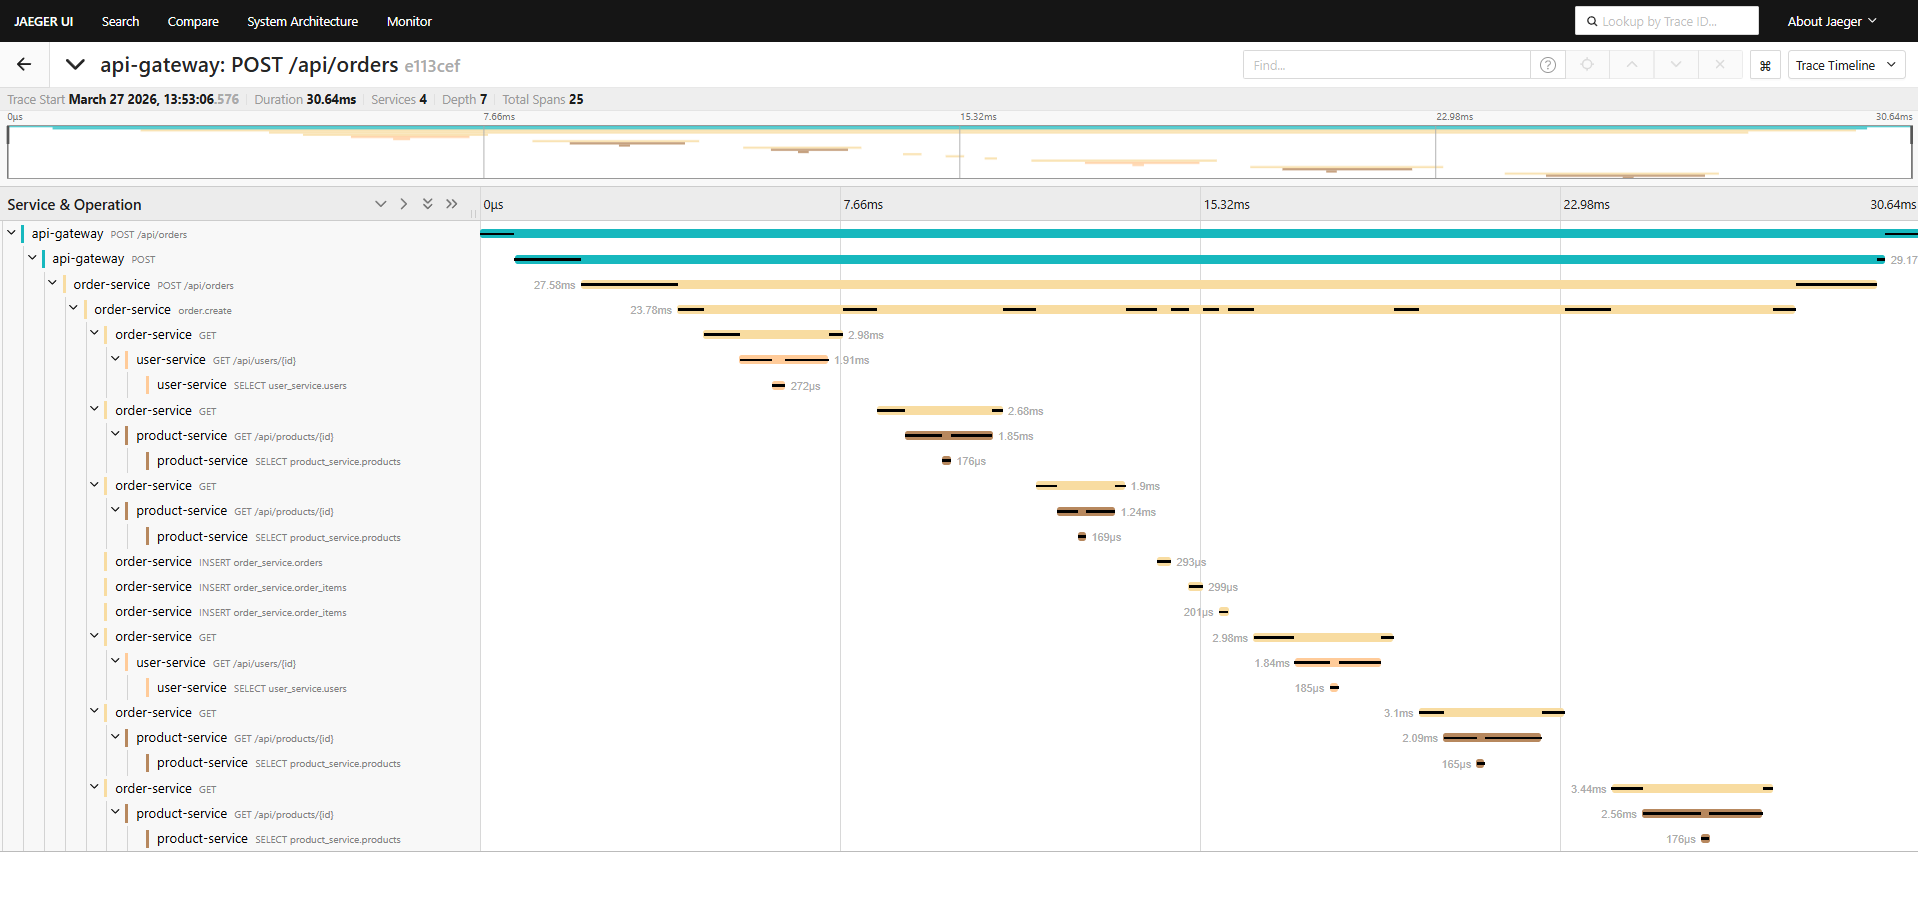
\includegraphics[width=\textwidth]{assets/jaeger/30-jaeger-trace-overview.png}
}{%
  \fbox{\parbox{0.92\textwidth}{\centering
  Guardar la captura de Jaeger en \texttt{docs/assets/jaeger/30-jaeger-trace-overview.png}\\
  para que esta figura se renderice automáticamente en el PDF.}}
}
\caption{Traza distribuida real de \texttt{POST /api/orders} en Jaeger. La vista temporal permite observar el span de entrada en \texttt{api-gateway}, la operación de negocio en \texttt{order-service} y las llamadas encadenadas a \texttt{user-service}, \texttt{product-service} y base de datos.}
\end{figure}

Esta figura tiene especial valor pedagógico porque resume, en una sola
pantalla, el resultado de todas las decisiones técnicas introducidas en
esta parte del laboratorio:

\begin{itemize}
\tightlist
\item
  dependencias de Spring para métricas y trazas
\item
  configuración de recursos y exportadores OTLP
\item
  despliegue del OTel Collector dentro de Kubernetes
\item
  propagación de contexto entre microservicios
\item
  instrumentación automática y manual combinadas
\end{itemize}

Dicho de otra forma, esta captura no es un adorno visual, sino la prueba
operativa de que la observabilidad distribuida está funcionando y de que
la llamada \texttt{POST /api/orders} puede explicarse extremo a extremo.

\begin{center}\rule{0.5\linewidth}{0.5pt}\end{center}

\chapter{Métricas de plataforma con Prometheus y
Grafana}\label{muxe9tricas-de-plataforma-con-prometheus-y-grafana}

\section{Prometheus como backend de
métricas y motor de scraping}\label{prometheus-como-backend-de-muxe9tricas}

Prometheus se desplegó con manifiestos propios y un scraping ajustado
tanto a la aplicación como al clúster. Esto permitió unificar en el
mismo backend:

\begin{itemize}
\tightlist
\item
  métricas de microservicios
\item
  métricas del nodo
\item
  métricas del clúster
\end{itemize}

Para entender bien esta parte conviene explicar qué significa
\textbf{scraping}. Prometheus no espera a que las aplicaciones le envíen
métricas de forma activa. Funciona al revés: el servidor Prometheus
consulta periódicamente unos endpoints HTTP y extrae de ellos el estado
actual de las métricas. Ese proceso de ir a un endpoint, leer su
contenido y almacenarlo como una nueva muestra temporal es precisamente
el scraping.

En este laboratorio, cada microservicio expone métricas en
\texttt{/actuator/prometheus} gracias a Spring Boot Actuator y
Micrometer. Prometheus visita ese endpoint a intervalos regulares,
parsea el texto en formato Prometheus y guarda series temporales con
pares \texttt{nombre + etiquetas + valor + timestamp}. Eso permite que,
con el paso del tiempo, Grafana pueda representar tendencias, tasas,
latencias o contadores acumulados.

Desde un punto de vista conceptual, el flujo es este:

\begin{enumerate}
\def\labelenumi{\arabic{enumi}.}
\tightlist
\item
  el microservicio publica métricas en un endpoint HTTP
\\item
  Prometheus conoce la URL de ese endpoint porque está declarada en su configuración
\item
  Prometheus consulta periódicamente ese endpoint
\item
  almacena las muestras como series temporales
\item
  Grafana consulta después esas series mediante PromQL
\end{enumerate}

Este diseño tiene varias ventajas didácticas. En primer lugar, hace muy
visible la diferencia entre \emph{emitir} métricas y \emph{almacenarlas}.
El microservicio solo expone su estado actual; quien lo recoge y lo
convierte en histórico es Prometheus. En segundo lugar, permite
incorporar al mismo backend tanto métricas de aplicación como métricas
de plataforma, siempre que exista un endpoint scrapeable.

\section{Grafana como capa de visualización y
alertado}\label{grafana-como-capa-de-visualizaciuxf3n-y-alertado}

Grafana se provisionó con:

\begin{itemize}
\tightlist
\item
  datasource Prometheus
\item
  proveedores de dashboards
\item
  dashboards importados y dashboards propios
\end{itemize}

Este punto tiene mucho valor práctico, porque enseña no solo a
``instalar Grafana'', sino a operarla correctamente como parte de una
plataforma reproducible.

\section{Métricas del clúster}\label{muxe9tricas-del-cluxfaster}

Además de la aplicación se incorporaron:

\begin{itemize}
\tightlist
\item
  \texttt{metrics-server}
\item
  \texttt{kube-state-metrics}
\item
  \texttt{node-exporter}
\end{itemize}

Con esto el laboratorio dejó de ser solo observabilidad de backend y
pasí a cubrir también la salud del clúster, que es una competencia
esencial en roles de plataforma.

\section{Configuración real de scraping en
Prometheus}\label{configuraciuxf3n-real-de-scraping-en-prometheus}

El \texttt{ConfigMap} de Prometheus contiene entradas muy expresivas del
enfoque seguido:

\begin{YamlCode}
- job_name: user-service
  metrics_path: /actuator/prometheus
  static_configs:
    - targets: ["user-service.default.svc.cluster.local:8080"]

- job_name: kube-state-metrics
  static_configs:
    - targets: ["kube-state-metrics.observability.svc.cluster.local:8080"]

- job_name: node-exporter
  static_configs:
    - targets: ["node-exporter.observability.svc.cluster.local:9100"]
\end{YamlCode}

Cada bloque de scraping define qué debe consultar Prometheus y cómo debe
nombrarlo internamente. Aquí aparecen varias ideas importantes:

\begin{itemize}
\tightlist
\item
  \texttt{job\_name}: agrupa y etiqueta el origen de las métricas. Es el
  nombre lógico con el que después se filtran series y se construyen
  paneles en Grafana.
\item
  \texttt{metrics\_path}: indica la ruta HTTP exacta que expone las
  métricas. En los microservicios de Spring es
  \texttt{/actuator/prometheus}.
\item
  \texttt{static\_configs}: lista los endpoints que Prometheus debe
  visitar. En este laboratorio se ha usado configuración estática para
  que el comportamiento sea fácil de entender y reproducir.
\end{itemize}

\section{Cómo funciona el scraping en la
práctica}\label{quuxe9-significa-esto-en-la-pruxe1ctica}

Prometheus no distingue ``mágicamente'' entre aplicación y plataforma.
Es el operador quien decide qué scrapea y cómo lo agrupa:

\begin{itemize}
\tightlist
\item
  los microservicios se scrapean por \texttt{/actuator/prometheus}
\item
  \texttt{kube-state-metrics} aporta estado lógico de objetos de
  Kubernetes, como pods, deployments o réplicas disponibles
\item
  \texttt{node-exporter} aporta métricas del nodo, como CPU, memoria o
  presión de recursos
\end{itemize}

Eso significa que el mismo Prometheus puede responder preguntas muy
 distintas entre sí. Por ejemplo:

\begin{itemize}
\tightlist
\item
  ``¿cuántas peticiones por segundo recibe \texttt{api-gateway}?''
\item
  ``¿cuánta heap JVM está consumiendo \texttt{order-service}?''
\item
  ``¿están todos los targets de scraping en estado \texttt{UP}?''
\item
  ``¿el nodo de Minikube está saturado?''
\end{itemize}

Esa mezcla es justo la que convierte a Prometheus en el backend central
de métricas del laboratorio. No solo recoge la salud de la aplicación,
sino también la del entorno que la ejecuta.

Un ejemplo sencillo de cómo se traduce esto en resultados sería el
siguiente:

\begin{PlainCode}
up{job="user-service"} = 1
http_server_requests_seconds_count{application="api-gateway",status="200"} = ...
process_resident_memory_bytes{job="order-service"} = ...
kube_deployment_status_replicas_available{deployment="api-gateway"} = ...
\end{PlainCode}

En ese pequeño conjunto ya se combinan cuatro perspectivas distintas:
conectividad del target, tráfico HTTP, consumo de memoria del proceso y
estado lógico del deployment en Kubernetes.

\section{Datasource provisionado en`r`nGrafana}\label{datasource-provisionado-en-grafana}

El datasource quedó definido de forma declarativa:

\begin{YamlCode}
datasources:
  - name: Prometheus
    uid: prometheus
    type: prometheus
    access: proxy
    url: http://prometheus.observability.svc.cluster.local:9090
    isDefault: true
\end{YamlCode}

\section{Evidencia visual de métricas,
dashboards y targets}\label{evidencia-visual-de-muxe9tricas-dashboards-y-targets}

La parte visual de esta capa se puede resumir con dos evidencias muy
complementarias. La primera muestra el dashboard operativo construido en
Grafana a partir de las series almacenadas en Prometheus. La segunda
muestra el estado de los targets, es decir, la confirmación de que el
scraping realmente está funcionando sobre los endpoints esperados.

\begin{figure}[H]
\centering
\IfFileExists{assets/grafana/20-grafana-dashboard-general.png}{%
  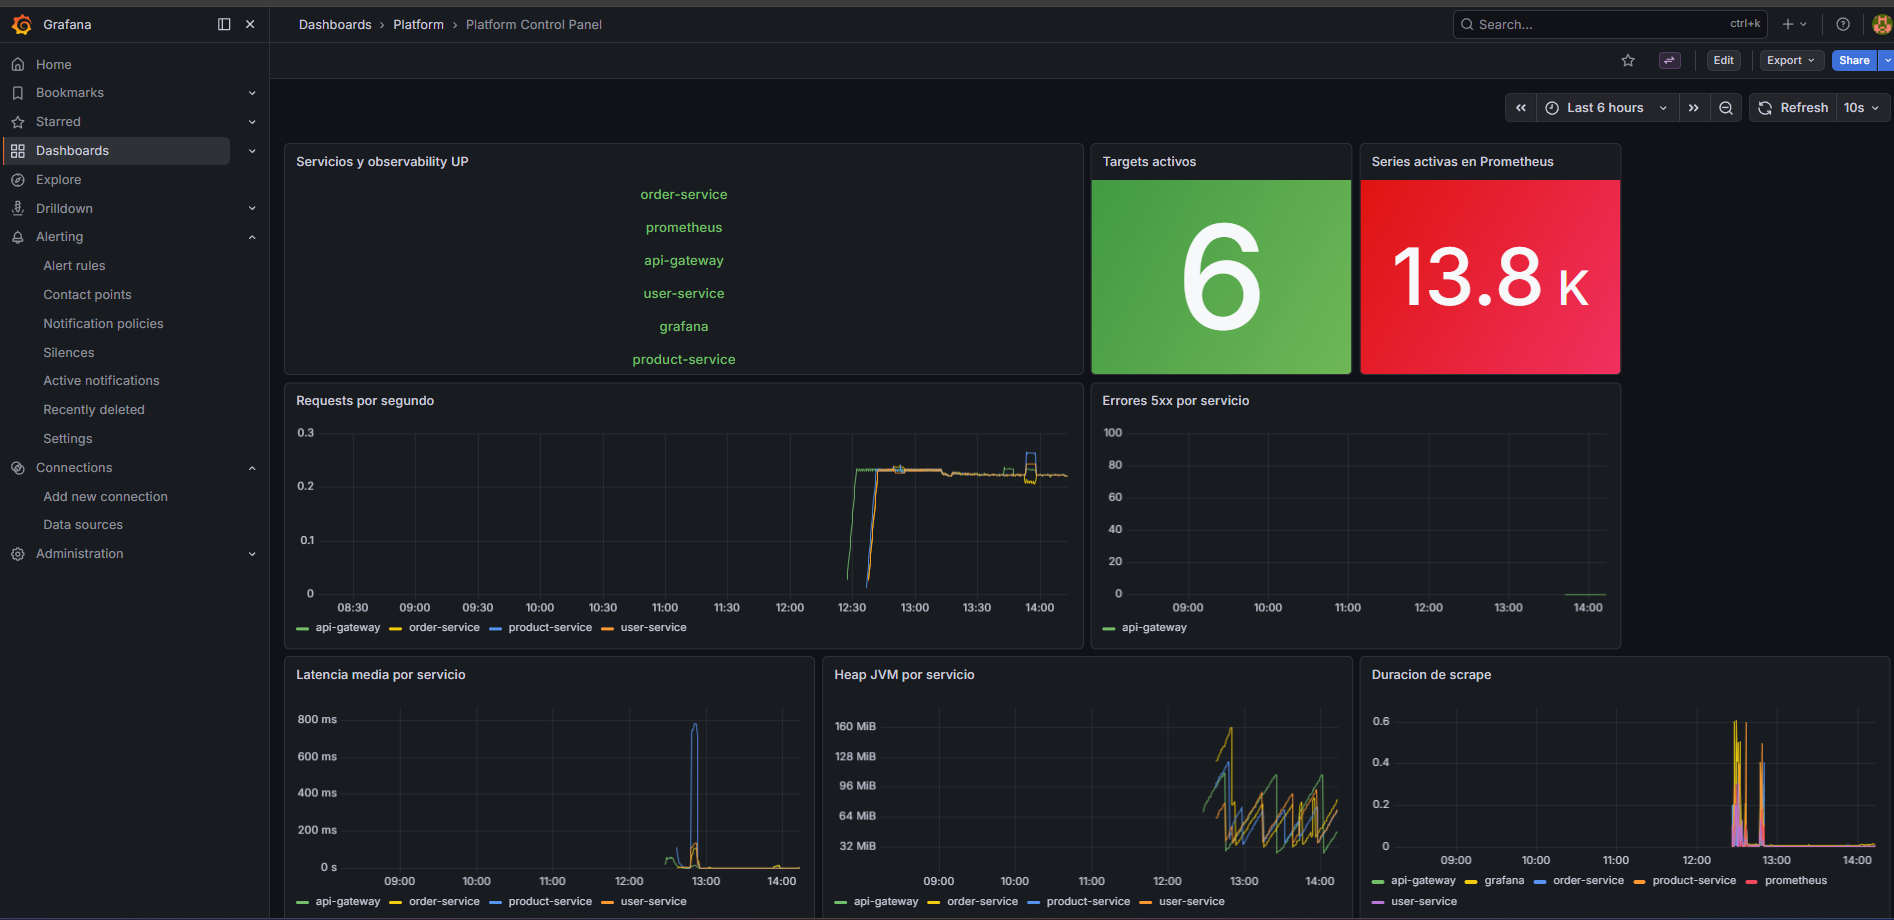
\includegraphics[width=\textwidth]{assets/grafana/20-grafana-dashboard-general.png}
}{%
  \fbox{\parbox{0.92\textwidth}{\centering
  Guardar la captura de Grafana en \texttt{docs/assets/grafana/20-grafana-dashboard-general.png}\\
  para que esta figura se renderice automáticamente en el PDF.}}
}
\caption{Dashboard general de plataforma en Grafana construido sobre Prometheus. En él se combinan paneles de disponibilidad, peticiones por segundo, errores 5xx, latencia, consumo de heap JVM y duración de scraping.}
\end{figure}

Este dashboard demuestra varias ideas a la vez. En un mismo panel se
juntan métricas de aplicación y métricas operativas: estado \texttt{UP}
de servicios, throughput HTTP, errores y comportamiento de memoria.
Dicho de otra forma, no se trata solo de ``tener gráficas'', sino de
poder responder preguntas operativas con una sola vista.

\begin{figure}[H]
\centering
\IfFileExists{assets/prometheus/22-prometheus-targets.png}{%
  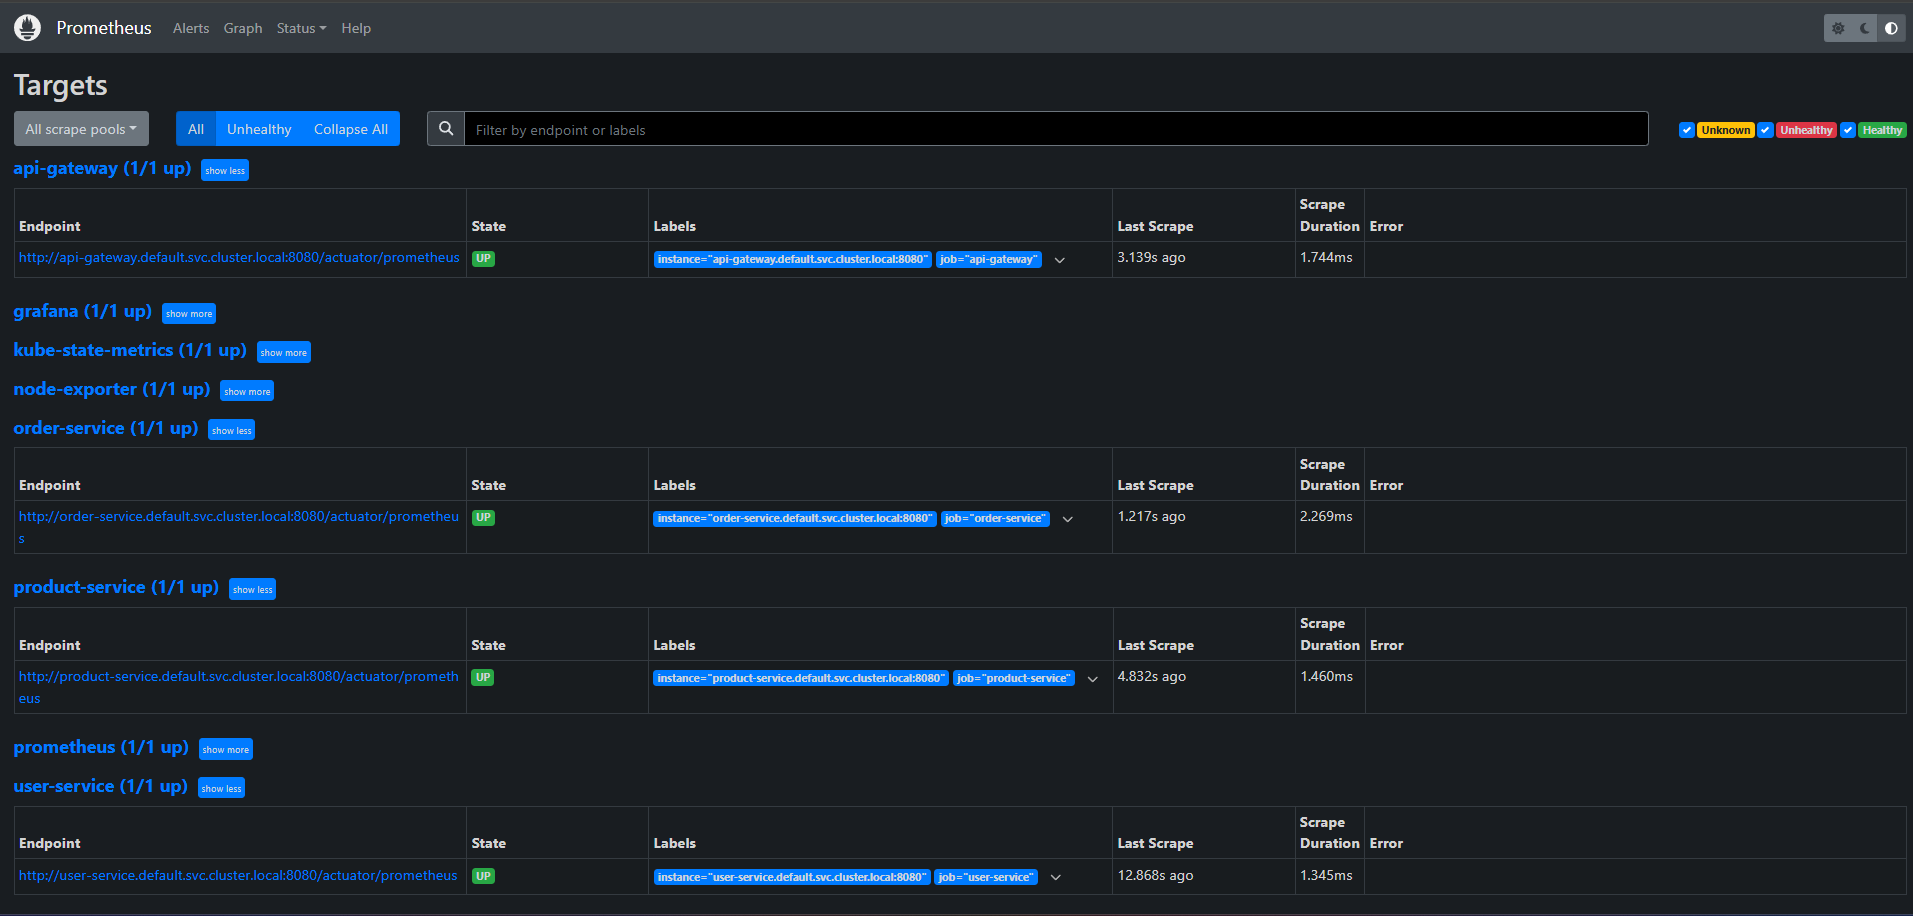
\includegraphics[width=\textwidth]{assets/prometheus/22-prometheus-targets.png}
}{%
  \fbox{\parbox{0.92\textwidth}{\centering
  Guardar la captura de Prometheus en \texttt{docs/assets/prometheus/22-prometheus-targets.png}\\
  para que esta figura se renderice automáticamente en el PDF.}}
}
\caption{Vista de targets de Prometheus en estado \texttt{UP}. Esta pantalla valida que el scraping alcanza correctamente a los microservicios instrumentados y a componentes de plataforma como \texttt{kube-state-metrics}, \texttt{node-exporter}, \texttt{grafana} y el propio \texttt{prometheus}.}
\end{figure}

Esta segunda figura es especialmente importante porque conecta la teoría 
del scraping con una evidencia operativa real.
No basta con escribir un \texttt{job\_name} en el \texttt{ConfigMap}; hay
que comprobar que Prometheus consigue resolver el endpoint, consultar la
ruta de métricas y almacenarla sin error. La columna de estado
\texttt{UP}, la duración del scrape y la ausencia de errores permiten
confirmarlo.

\begin{center}\rule{0.5\linewidth}{0.5pt}\end{center}

\chapter{Logging centralizado y logs
estructurados}\label{logging-centralizado-y-logs-estructurados}

\section{Introducción del stack
Elastic}\label{introducciuxf3n-del-stack-elastic}

Para cubrir la dimensión de logs del laboratorio se desplegó un stack
basado en tecnologías Elastic. Este bloque resuelve una necesidad muy
concreta: almacenar, indexar, enriquecer y consultar eventos generados
por los microservicios y por la propia plataforma. En un sistema
mínimamente distribuido, leer la salida de consola de un único pod deja
rápidamente de ser suficiente. En cuanto intervienen varios servicios,
trazas concurrentes y reinicios de contenedores, hace falta una capa de
logging centralizado que permita responder preguntas como estas:

\begin{itemize}
\tightlist
\item
  qué servicio emitió el evento
\item
  en qué instante exacto ocurrió
\item
  qué nivel de severidad tenía
\item
  a qué pod, namespace y contenedor pertenecía
\item
  si el evento se relaciona con una traza concreta
\end{itemize}

Para cubrir esa necesidad se desplegaron estos componentes:

\begin{itemize}
\tightlist
\item
  \textbf{Elasticsearch}, como motor de almacenamiento, indexación y
  búsqueda de documentos.
\item
  \textbf{Kibana}, como interfaz de exploración, filtrado, visualización
  y alertado sobre los logs indexados.
\item
  \textbf{Filebeat}, como agente ligero encargado de leer los logs de
  contenedores en Kubernetes y enviarlos aguas arriba.
\item
  \textbf{ECK} (\emph{Elastic Cloud on Kubernetes}), como operador que
  simplifica el despliegue y la gestión de los recursos Elastic dentro
  del clúster.
\end{itemize}

La elección de este stack no responde solo a su popularidad. También es
especialmente útil en un laboratorio didáctico porque obliga a entender
varias capas de observabilidad a la vez: formato de los logs,
recolección, enriquecimiento con metadatos, indexación, búsqueda por
campos y correlación con métricas y trazas.

\section{Qué es Elasticsearch y por qué se usa en este
proyecto}\label{quuxe9-es-elasticsearch-y-por-quuxe9-se-usa-en-este-proyecto}

Elasticsearch es un motor distribuido orientado a almacenar documentos y
consultarlos de forma eficiente. En este laboratorio cada evento de log
acaba convirtiéndose en un documento indexado con campos estructurados,
por ejemplo \texttt{service.name}, \texttt{log.level},
\texttt{trace\_id}, \texttt{message} o metadatos de Kubernetes.

Eso cambia por completo la forma de trabajar con logs. En lugar de tener
una secuencia lineal de texto, Elasticsearch permite hacer búsquedas y
agregaciones sobre campos concretos. Por ejemplo, se puede pedir:

\begin{itemize}
\tightlist
\item
  todos los eventos \texttt{ERROR} del \texttt{order-service}
\item
  todos los logs que comparten un mismo \texttt{trace\_id}
\item
  todos los eventos emitidos por un pod concreto
\item
  la distribución temporal de errores en una franja horaria
\end{itemize}

Desde el punto de vista de arquitectura, Elasticsearch actúa como el
backend persistente de la capa de logs. Filebeat le entrega eventos ya
procesados y Kibana consulta después esa información para mostrarla,
filtrarla y construir reglas de alerta.

\section{Qué es Kibana y qué aporta más allá de ``ver
logs'}\label{quuxe9-es-kibana-y-quuxe9-aporta-muxe1s-alluxe1-de-ver-logs}

Kibana es la interfaz visual del stack Elastic. Su valor no está solo en
mostrar eventos, sino en permitir explorarlos con contexto. En la vista
\emph{Discover}, por ejemplo, el operador puede:

\begin{itemize}
\tightlist
\item
  seleccionar un \emph{data view}
\item
  filtrar por campos estructurados
\item
  fijar una ventana temporal
\item
  ordenar por marca de tiempo
\item
  destacar columnas relevantes como \texttt{service.name},
  \texttt{log.level} o \texttt{trace\_id}
\end{itemize}

En la práctica, Kibana convierte una colección de documentos en una
herramienta de análisis operacional. En este proyecto sirve para
entender el comportamiento del flujo de negocio, localizar errores,
seguir dependencias entre microservicios y enlazar una línea de log con
una traza completa en Jaeger.

\section{Qué es Filebeat y cómo se conecta con los
servicios}\label{quuxe9-es-filebeat-y-cuxf3mo-se-conecta-con-los-servicios}

Filebeat es un agente de recolección de logs. No se integra dentro del
código Java ni llama a los microservicios por HTTP. Su papel es otro:
lee los ficheros de log generados por los contenedores del clúster,
extrae cada evento, lo procesa y lo reenvía a Elasticsearch.

En Kubernetes, los contenedores escriben normalmente a \texttt{stdout} y
\texttt{stderr}. El runtime del contenedor persiste esa salida en rutas
bajo \texttt{/var/log/containers}. Filebeat se despliega como agente del
clúster y observa precisamente esas rutas. Después aplica procesadores
que interpretan el formato del evento, expanden el JSON y añaden
metadatos como namespace, pod, labels o nombre del contenedor.

Esto significa que la conexión entre Filebeat y los servicios es
\textbf{indirecta pero continua}: los microservicios solo escriben logs a
consola, y Filebeat se encarga de recogerlos sin modificar el código de
negocio.

\section{Qué es ECK y por qué se utilizó en el
laboratorio}\label{quuxe9-es-eck-y-por-quuxe9-se-utilizuxf3-en-el-laboratorio}

ECK significa \emph{Elastic Cloud on Kubernetes}. Se trata del operador
oficial de Elastic para Kubernetes. Su función es traducir recursos de
alto nivel, como clústeres Elasticsearch o instancias de Kibana, en los
objetos nativos que Kubernetes necesita realmente: pods, statefulsets,
servicios, secretos, certificados y configuración asociada.

En un laboratorio pequeño podría haberse optado por manifiestos
manuales, pero ECK aporta varias ventajas didácticas y operativas:

\begin{itemize}
\tightlist
\item
  automatiza tareas de despliegue y configuración seguras
\item
  gestiona certificados y comunicación TLS entre componentes
\item
  simplifica la administración de credenciales
\item
  acerca el laboratorio a un modelo real de operación en Kubernetes
\end{itemize}

Por tanto, ECK no ``genera logs', pero sí habilita la forma ordenada y
reproducible de desplegar la plataforma Elastic dentro del clúster.

\section{Primer problema: tener logs no significa tener
observabilidad}\label{primer-problema-tener-logs-no-significa-tener-observabilidad}

En las primeras iteraciones, Kibana recibía datos pero no resultaba útil
para investigar flujo de negocio. Muchos eventos visibles eran puramente
de infraestructura. El problema real no era Filebeat ni Elasticsearch,
sino la calidad de los logs emitidos por la aplicación.

\section{Introducción de logging de
negocio}\label{introducciuxf3n-de-logging-de-negocio}

Se añadieron logs de negocio en servicios clave, especialmente en los
puntos donde el flujo entra o donde existen dependencias downstream. Con
ello empezaron a aparecer mensajes que sí describían acciones relevantes
del sistema.

\section{Limitaciones del texto
plano}\label{limitaciones-del-texto-plano}

Aunque los logs de negocio mejoraron la visibilidad, seguían siendo
difíciles de explotar:

\begin{itemize}
\tightlist
\item
  no era trivial filtrar por \texttt{service.name}
\item
  no era trivial filtrar por \texttt{log.level}
\item
  la correlación con trazas era pobre
\end{itemize}

Por eso se decidió migrar a logs ECS JSON.

\section{ECS JSON}\label{ecs-json}

Los servicios incorporaron \texttt{logback-ecs-encoder}, lo que permitió
emitir eventos estructurados con campos como:

\begin{itemize}
\tightlist
\item
  \texttt{@timestamp}
\item
  \texttt{service.name}
\item
  \texttt{service.environment}
\item
  \texttt{log.level}
\item
  \texttt{log.logger}
\item
  \texttt{message}
\item
  \texttt{trace\_id}
\item
  \texttt{span\_id}
\end{itemize}

Este cambio marcó uno de los hitos más importantes del laboratorio: los
logs pasaron de ser texto ``legible'' a ser datos realmente explotables.

\section{Adaptación de Filebeat}\label{adaptaciuxf3n-de-filebeat}

Filebeat se ajustó para detectar y decodificar JSON dentro del campo
\texttt{message}, expandiendo los campos y enriqueciendo el evento con
metadatos de Kubernetes. De este modo Kibana pudo consultar directamente
propiedades estructuradas.

\section{Correlación Kibana -\textgreater{}
Jaeger}\label{correlaciuxf3n-kibana---jaeger}

Una vez disponible \texttt{trace\_id} en logs, el flujo de
troubleshooting ganó mucha potencia:

\begin{enumerate}
\def\labelenumi{\arabic{enumi}.}
\tightlist
\item
  localizar un evento en Kibana\\
\item
  extraer el \texttt{trace\_id}\\
\item
  abrir Jaeger\\
\item
  buscar la traza exacta
\end{enumerate}

Este punto convierte el laboratorio en algo mucho más valioso que una
simple agregación de logs.

\section{\texorpdfstring{Configuración real de
\texttt{logback-spring.xml}}{11.8 Configuración real de logback-spring.xml}}\label{configuraciuxf3n-real-de-logback-spring.xml}

Los cuatro servicios comparten una estructura muy parecida para emitir
ECS JSON. El patrón básico es:

\begin{XmlCode}
<configuration>
    <springProperty scope="context" name="serviceName" source="spring.application.name"/>

    <appender name="ECS_JSON_CONSOLE" class="ch.qos.logback.core.ConsoleAppender">
        <encoder class="co.elastic.logging.logback.EcsEncoder">
            <serviceName>${serviceName}</serviceName>
            <serviceEnvironment>minikube</serviceEnvironment>
            <includeOrigin>true</includeOrigin>
        </encoder>
    </appender>

    <logger name="com.mercadona.devops" level="INFO"/>

    <root level="INFO">
        <appender-ref ref="ECS_JSON_CONSOLE"/>
    </root>
</configuration>
\end{XmlCode}

\section{Qué hace cada bloque de este
logback}\label{quuxe9-hace-cada-bloque-de-este-logback}

\begin{itemize}
\tightlist
\item
  \texttt{springProperty}: reutiliza \texttt{spring.application.name}
  como nombre de servicio.
\item
  \texttt{ConsoleAppender}: escribe en \texttt{stdout}, que es lo
  esperable en contenedores.
\item
  \texttt{EcsEncoder}: transforma cada evento de log en un documento
  JSON con estructura ECS.
\item
  \texttt{serviceEnvironment}: añade contexto de entorno.
\item
  \texttt{includeOrigin=true}: agrega información de origen útil para
  debugging.
\end{itemize}

Esta configuración es un excelente ejemplo de una buena práctica
moderna: en contenedores, lo habitual es escribir a consola y dejar que
un agente externo recoja y enrute los logs.

\section{Ejemplo de log útil en código de
negocio}\label{ejemplo-de-log-uxfatil-en-cuxf3digo-de-negocio}

En \texttt{OrderServiceImpl} aparecen logs que sí ayudan a entender el
comportamiento:

\begin{JavaCode}
log.info("Fetching user {} from user-service", userId);
...
log.error("User service unavailable while fetching user {}", userId, exception);
\end{JavaCode}

\section{Por qué estos logs sí aportan
valor}\label{por-quuxe9-estos-logs-suxed-aportan-valor}

\begin{itemize}
\tightlist
\item
  describen una acción concreta
\item
  indican a qué dependencia se está llamando
\item
  diferencian éxito, degradación y fallo
\item
  se correlacionan con spans y métricas
\end{itemize}

Un junior suele tender a loggear solo ``entró en método X''. En cambio,
aquí el foco se puso en eventos de negocio y de integración.

\section{Filebeat como puente entre contenedores y
Elasticsearch}\label{filebeat-como-puente-entre-contenedores-y-elasticsearch}

La configuración relevante de Filebeat es esta:

\begin{YamlCode}
filebeat.inputs:
  - type: filestream
    id: kubernetes-container-logs
    prospector.scanner.symlinks: true
    parsers:
      - container: ~
    paths:
      - /var/log/containers/*.log
processors:
  - decode_json_fields:
      when:
        regexp:
          message: '^\{'
      fields: ["message"]
      target: ""
      overwrite_keys: true
      add_error_key: true
      expand_keys: true
  - add_kubernetes_metadata: {}
\end{YamlCode}

\section{Cómo se interpreta esta
configuración}\label{cuxf3mo-se-interpreta-esta-configuraciuxf3n}

\begin{itemize}
\tightlist
\item
  \texttt{filestream}: lector moderno de logs en Filebeat.
\item
  \texttt{paths}: apunta a logs de contenedores de Kubernetes.
\item
  \texttt{parsers.container}: interpreta el formato de log del runtime.
\item
  \texttt{decode\_json\_fields}: convierte el JSON emitido por Logback
  en campos de Elasticsearch.
\item
  \texttt{add\_kubernetes\_metadata}: añade namespace, pod, labels y
  otra información útil.
\end{itemize}

Este paso es crucial. Sin \texttt{decode\_json\_fields}, el log llegaría
como texto plano dentro de \texttt{message}, y se perdería gran parte de
la utilidad del formato ECS.

Desde un punto de vista operativo, Filebeat hace cuatro tareas seguidas:
lee, interpreta, enriquece y reenvía. Primero detecta una nueva línea de
log en el fichero del contenedor. Después comprueba si la línea contiene
JSON. Si es así, expande ese contenido en campos propios del documento.
A continuación añade información de Kubernetes. Finalmente entrega el
evento a Elasticsearch para que pueda ser indexado.

Ese pipeline convierte una simple línea de salida estándar en un evento
mucho más rico. Gracias a ello, Kibana no solo muestra un mensaje, sino
un documento con contexto de plataforma y de aplicación. En un informe
didáctico conviene remarcar esta idea: el valor del stack no depende de
una única pieza, sino del encadenamiento correcto entre emisor,
recolector, almacenamiento e interfaz de consulta.

\section{Cómo recorre un log todo el pipeline hasta
Kibana}\label{cuxf3mo-recorre-un-log-todo-el-pipeline-hasta-kibana}

El recorrido completo de un evento en este laboratorio puede resumirse
así:

\begin{enumerate}
\def\labelenumi{\arabic{enumi}.}
\tightlist
\item
  un microservicio emite un log ECS JSON por consola
\item
  Kubernetes lo persiste como log del contenedor
\item
  Filebeat lee el evento desde \texttt{/var/log/containers}
\item
  Filebeat expande el JSON y añade metadatos de Kubernetes
\item
  Elasticsearch indexa el documento
\item
  Kibana consulta ese índice y permite filtrarlo por campos
\end{enumerate}

Este modelo tiene una implicación importante: los servicios no necesitan
saber nada de Kibana ni de Elasticsearch. Solo necesitan emitir logs con
un formato coherente. Todo lo demás lo resuelve la canalización de
observabilidad.

\section{Qué campos gana Kibana gracias a
ECS}\label{quuxe9-campos-gana-kibana-gracias-a-ecs}

Cuando el pipeline de logging está bien montado, Kibana puede filtrar
directamente por:

\begin{itemize}
\tightlist
\item
  \texttt{service.name}
\item
  \texttt{service.environment}
\item
  \texttt{log.level}
\item
  \texttt{log.logger}
\item
  \texttt{trace\_id}
\item
  \texttt{span\_id}
\end{itemize}

Ese es el salto de calidad real del proyecto. No se trata solo de
``guardar logs'', sino de convertir los logs en datos consultables.

\section{Evidencia visual de logs estructurados en
Kibana}\label{evidencia-visual-de-logs-estructurados-en-kibana}

La siguiente captura muestra el resultado práctico del pipeline de
logging ya completo. En ella se observan eventos procedentes de varios
microservicios, columnas con \texttt{service.name},
\texttt{log.level} y \texttt{trace\_id}, y una vista temporal que permite
entender cómo se concentra la actividad en una franja concreta. Esta
imagen es especialmente valiosa porque demuestra que la plataforma no
solo almacena logs, sino que los presenta con el suficiente contexto
como para investigar comportamiento distribuido.

\begin{figure}[H]
\centering
\IfFileExists{assets/kibana/40-kibana-discover-logs.png}{%
  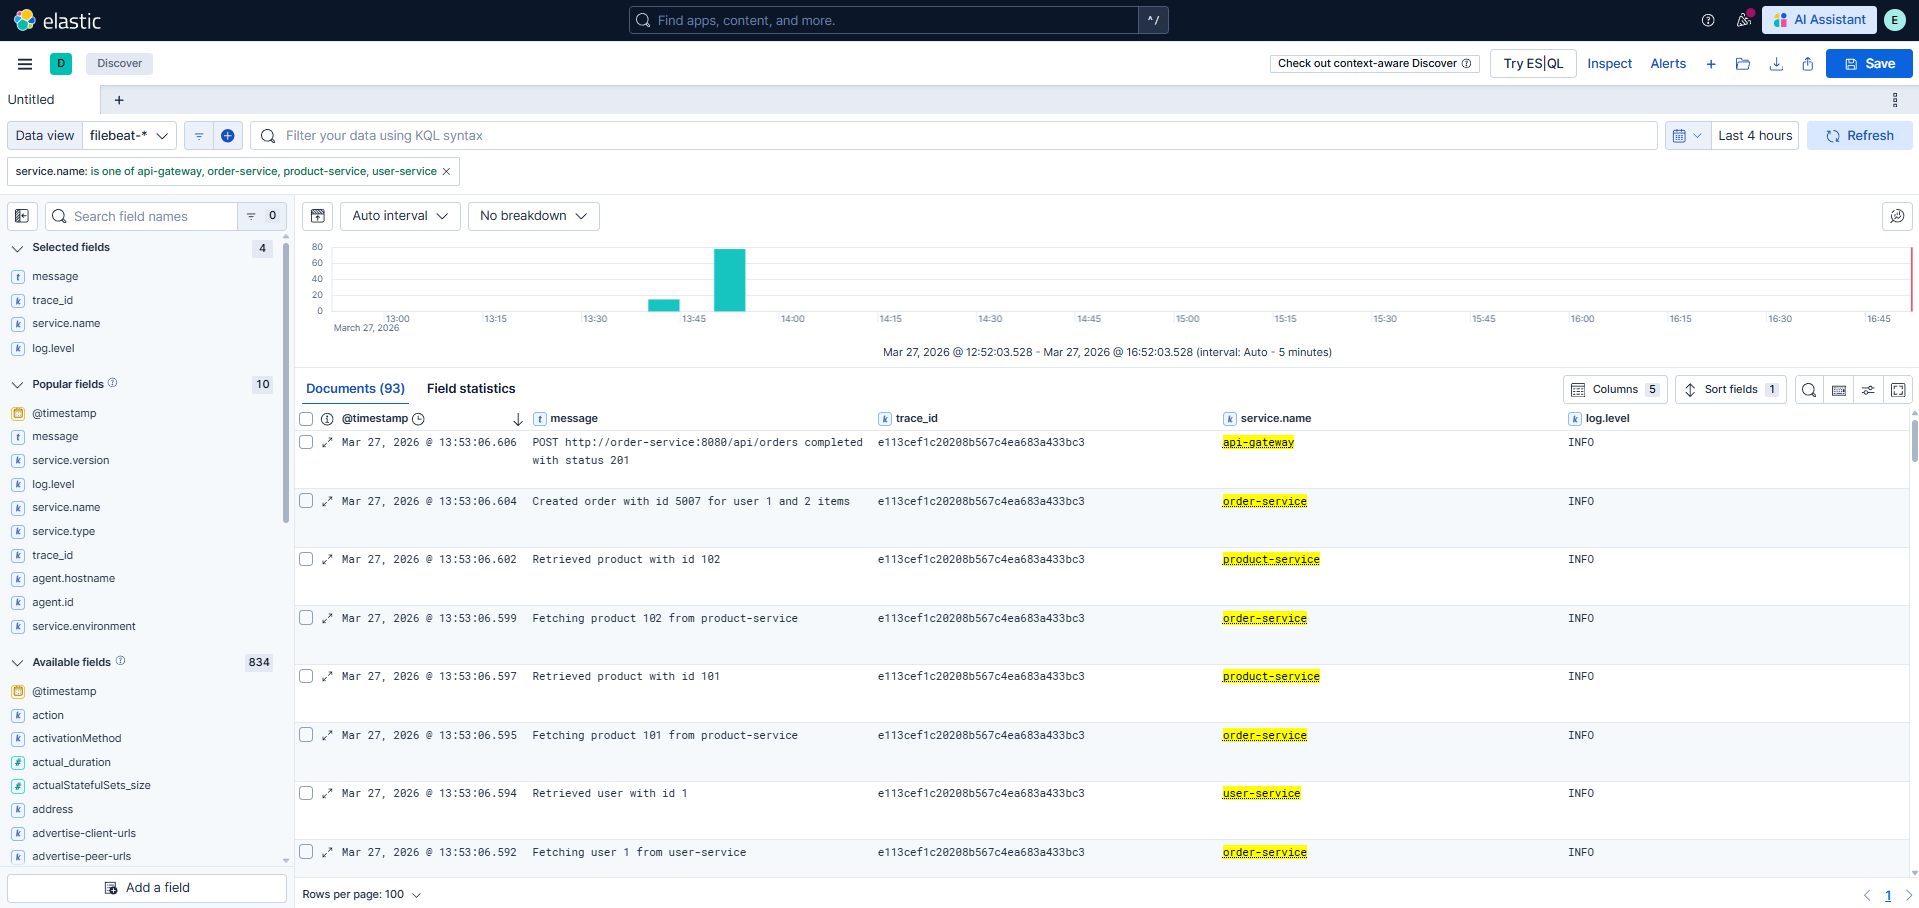
\includegraphics[width=\textwidth]{assets/kibana/40-kibana-discover-logs.png}%
}{%
  \fbox{\parbox{0.92\textwidth}{%
  \textbf{Falta la imagen real:} colocar aquí
  \texttt{assets/kibana/40-kibana-discover-logs.png}.%
  }}%
}
\caption{Vista \emph{Discover} de Kibana con logs de varios microservicios y campos estructurados como \texttt{service.name}, \texttt{log.level} y \texttt{trace\_id}, útiles para correlación operativa.}
\label{fig:kibana-discover-logs}
\end{figure}

\begin{center}\rule{0.5\linewidth}{0.5pt}\end{center}

\chapter{Alertado por métricas y por
logs}\label{alertado-por-muxe9tricas-y-por-logs}

\section{Alerta de métricas en
Grafana}\label{alerta-de-muxe9tricas-en-grafana}

Se implementó una alerta orientada a detectar caídas de microservicios,
utilizando la métrica \texttt{up} de Prometheus. La validación se
realizó provocando una situación real de no disponibilidad.

\section{Alerta de logs en Kibana}\label{alerta-de-logs-en-kibana}

Se implementó una regla que detecta logs \texttt{ERROR} emitidos por
cualquiera de los microservicios. Esto permitió demostrar una línea de
observabilidad complementaria:

\begin{itemize}
\tightlist
\item
  fallo funcional
\item
  emisión de error
\item
  almacenamiento en Elasticsearch
\item
  visualización en Kibana
\item
  activación de una regla
\end{itemize}

\section{Aprendizaje principal}\label{aprendizaje-principal-1}

Métricas y logs no compiten: se complementan. Las métricas sirven para
detectar comportamiento anómalo agregado; los logs ayudan a explicar qué
ocurrió; las trazas muestran el recorrido de una petición concreta.

\section{Ejemplo didáctico de alerta de
métricas}\label{ejemplo-diduxe1ctico-de-alerta-de-muxe9tricas}

La alerta \texttt{MicroserviceDown} se apoyó en una idea muy simple y
potente: si Prometheus deja de ver un target, probablemente el servicio
está caído o inaccesible.

Consulta representativa:

\begin{PlainCode}
up{job=~"api-gateway|user-service|product-service|order-service"}
\end{PlainCode}

Interpretación:

\begin{itemize}
\tightlist
\item
  \texttt{up\ =\ 1}: Prometheus ha podido scrapear el target.
\item
  \texttt{up\ =\ 0}: el scrape ha fallado.
\end{itemize}

Este ejemplo es excelente porque enseña que una
alerta efectiva no siempre necesita lógica compleja. A veces basta con
entender bien una métrica base.

\section{Ejemplo didáctico de alerta de
logs}\label{ejemplo-diduxe1ctico-de-alerta-de-logs}

La regla de Kibana para errores se apoyó en una consulta del tipo:

\begin{PlainCode}
log.level : "ERROR" and service.name : ("api-gateway" or "user-service" or "product-service" or "order-service")
\end{PlainCode}

Qué enseña esta consulta:

\begin{itemize}
\tightlist
\item
  \texttt{log.level} solo existe porque el logging es estructurado.
\item
  \texttt{service.name} solo es filtrable porque se ha normalizado el
  formato del log.
\item
  sin ECS JSON, esta regla sería mucho más frágil.
\end{itemize}

\section{Diferencia pedagógica entre ambas
alertas}\label{diferencia-pedaguxf3gica-entre-ambas-alertas}

{\def\LTcaptype{none} % do not increment counter
\begin{longtable}[]{@{}
  >{\raggedright\arraybackslash}p{(\linewidth - 6\tabcolsep) * \real{0.2500}}
  >{\raggedright\arraybackslash}p{(\linewidth - 6\tabcolsep) * \real{0.2500}}
  >{\raggedright\arraybackslash}p{(\linewidth - 6\tabcolsep) * \real{0.2500}}
  >{\raggedright\arraybackslash}p{(\linewidth - 6\tabcolsep) * \real{0.2500}}@{}}
\toprule\noalign{}
\begin{minipage}[b]{\linewidth}\raggedright
Alerta
\end{minipage} & \begin{minipage}[b]{\linewidth}\raggedright
Fuente
\end{minipage} & \begin{minipage}[b]{\linewidth}\raggedright
Qué detecta
\end{minipage} & \begin{minipage}[b]{\linewidth}\raggedright
Qué no explica por sí sola
\end{minipage} \\
\midrule\noalign{}
\endhead
\bottomrule\noalign{}
\endlastfoot
Grafana \texttt{MicroserviceDown} & Métricas & indisponibilidad o fallo
de scrape & la causa concreta \\
Kibana \texttt{ErrorLogsByService} & Logs & errores de aplicación
visibles en logs & salud global del target \\
\end{longtable}
}

Esta comparación merece estar explícita en la memoria, porque enseña a
elegir el backend adecuado según el tipo de señal que se quiere
explotar.


\chapter{GitLab self-managed dentro del
laboratorio}\label{gitlab-self-managed-dentro-del-laboratorio}

\section{Motivación}\label{motivaciuxf3n}

Una vez establecida la observabilidad, el siguiente salto natural fue
incorporar una capa real de CI/CD. En lugar de depender de GitLab.com u
otro SaaS, se optó por desplegar GitLab CE dentro del propio Minikube.

Esta decisión tiene una carga didáctica importante. No se trataba solo
de tener un repositorio Git, sino de estudiar cómo conviven en un mismo
laboratorio el código fuente, la gestión del proyecto, las pipelines, el
runner, el registry y el despliegue. Al introducir GitLab dentro del
clúster, el proyecto dejó de centrarse únicamente en la aplicación y
pasó a incluir también una plataforma de entrega continua operativa.

\section{Qué es GitLab CE y qué aporta en este
proyecto}\label{quuxe9-es-gitlab-ce-y-quuxe9-aporta-en-este-proyecto}

GitLab CE significa \emph{GitLab Community Edition}. Es la edición libre
y autoalojada del producto, suficiente para cubrir la mayor parte de las
necesidades que interesan en este laboratorio: control de versiones,
interfaz web del repositorio, pipelines CI/CD, gestión de runners y
registro de imágenes.

Conviene detenerse un momento en qué significa realmente \emph{Community
Edition}. No es una edición ``demo' ni un visor del repositorio,
sino un producto completo que permite gestionar el ciclo de vida del
software. La diferencia fundamental frente a un servicio SaaS es que aquí
la plataforma se administra dentro del propio clúster: el equipo decide
cómo exponerla, cómo integrarla con el runner, cómo conectarla con el
registry y cómo resolver sus problemas de red, persistencia o salud.

En este proyecto GitLab CE cumple varios papeles a la vez:

\begin{itemize}
\tightlist
\item
  actúa como servidor Git del repositorio principal
\item
  ofrece la interfaz web para navegar el código, commits, ramas,
  pipelines y configuración del proyecto
\item
  coordina la ejecución de la pipeline definida en
  \texttt{.gitlab-ci.yml}
\item
  centraliza credenciales y variables de CI/CD
\item
  expone el Container Registry usado para almacenar las imágenes
  generadas por la pipeline
\item
  sirve como punto único de verdad para enlazar commit, pipeline, imagen
  y despliegue
\end{itemize}

En otras palabras, GitLab es el plano de control del ciclo de vida de
entrega: recibe cambios, desencadena automatización, muestra resultados
y conserva artefactos e imágenes. Esto transforma por completo el
laboratorio: ya no se trata solo de varios microservicios desplegados,
sino de una plataforma capaz de recibir código, validarlo, convertirlo
en una imagen y desplegarlo con trazabilidad.

\section{Qué partes tiene GitLab dentro de este
laboratorio}\label{quuxe9-partes-tiene-gitlab-dentro-de-este-laboratorio}

Cuando se despliega GitLab en Kubernetes no aparece un único pod mágico.
Lo que se obtiene es un conjunto de componentes que colaboran entre sí.
Los más relevantes en este laboratorio son estos:

\begin{itemize}
\tightlist
\item
  \textbf{webservice}: sirve la interfaz web y atiende las peticiones
  HTTP del usuario. Es la cara visible de GitLab para navegar el
  repositorio, lanzar pipelines o consultar el estado del runner.
\item
  \textbf{Gitaly}: gestiona operaciones del repositorio Git en backend,
  como lecturas, escrituras y acceso eficiente a datos del repositorio.
  Cuando GitLab necesita mostrar commits, ramas o leer un repo, Gitaly
  participa de forma decisiva.
\item
  \textbf{PostgreSQL}: almacena la base de datos interna de GitLab,
  donde viven configuraciones, usuarios, permisos, pipelines, registros
  y metadatos de proyecto.
\item
  \textbf{Redis}: soporta caché, colas y comunicación rápida entre
  componentes. Ayuda a desacoplar partes de la plataforma y a evitar que
  todo pase por consultas de base de datos.
\item
  \textbf{Registry}: publica y sirve imágenes de contenedor del
  proyecto. Es el puente entre la parte de CI y el runtime de
  Kubernetes.
\item
  \textbf{Ingress}: expone GitLab hacia el exterior del clúster y hace
  posible que un usuario entre desde Windows a la interfaz web.
\end{itemize}

Esta descomposición es importante porque muestra
que una plataforma de desarrollo moderna no es un binario único, sino un
conjunto de servicios coordinados. También ayuda a entender por qué en
esta fase aparecieron problemas reales de red, TLS, permisos y salud de
pods: si falla Gitaly, por ejemplo, la web puede devolver errores 500
aunque la interfaz siga respondiendo; si falla el registry, la pipeline
puede construir pero no publicar imágenes; si falla el ingress, GitLab
puede seguir sano internamente pero dejar de ser accesible desde fuera.

\section{Configuración principal}\label{configuraciuxf3n-principal}

La instalación se apoyó en:

\begin{itemize}
\tightlist
\item
  \texttt{deploy/gitlab/values-minikube.yaml}
\item
  \texttt{deploy/gitlab/values-local.yaml}
\end{itemize}

La configuración local se orientó a:

\begin{itemize}
\tightlist
\item
  edición CE
\item
  dominio basado en \texttt{nip.io}
\item
  desactivación del Prometheus y Grafana incluidos en el chart
\item
  uso de la instancia ya existente de observabilidad del laboratorio
\end{itemize}
\section{Dificultades de acceso}\label{dificultades-de-acceso}

El acceso a GitLab desde Windows en un entorno Minikube con driver
Docker no fue inmediato. Hubo que combinar:

\begin{itemize}
\tightlist
\item
  \texttt{port-forward} del ingress controller
\item
  entrada en \texttt{hosts}
\item
  acceso por \texttt{https://gitlab.192.168.49.2.nip.io:8443}
\end{itemize}

Este punto es especialmente interesante en una memoria técnica porque
muestra una idea importante: muchas dificultades de plataforma tienen
que ver con red y exposición de servicios, no con la aplicación en sí.

\section{Configuración local de GitLab}\label{configuraciuxf3n-local-de-gitlab}

El override principal quedó en \texttt{deploy/gitlab/values-local.yaml}:

\begin{YamlCode}
global:
  edition: ce
  hosts:
    domain: 192.168.49.2.nip.io
    externalIP: 192.168.49.2
  grafana:
    enabled: false

prometheus:
  install: false

gitlab-runner:
  install: false
\end{YamlCode}

Esta configuración expresa varias decisiones importantes del laboratorio:

\begin{itemize}
\tightlist
\item
  \texttt{edition: ce} selecciona GitLab Community Edition.
\item
  \texttt{domain} y \texttt{externalIP} definen cómo se construyen los
  hosts públicos del despliegue.
\item
  \texttt{grafana.enabled: false} y \texttt{prometheus.install: false}
  evitan duplicar la observabilidad ya existente en el laboratorio.
\item
  \texttt{gitlab-runner.install: false} separa el servidor GitLab del
  runner, de modo que este último puede configurarse e instalarse de
  forma controlada con su propio chart.
\end{itemize}

\section{Interfaz del proyecto en GitLab}\label{interfaz-del-proyecto-en-gitlab}

La siguiente captura muestra el repositorio principal del laboratorio ya
importado en GitLab. Esta evidencia es útil porque confirma que GitLab
no fue una instalación aislada de infraestructura, sino el origen real
para commits, ramas, pipeline, Container Registry y despliegue.

\begin{figure}[H]
\centering
\IfFileExists{assets/gitlab/50-gitlab-home-project.png}{%
  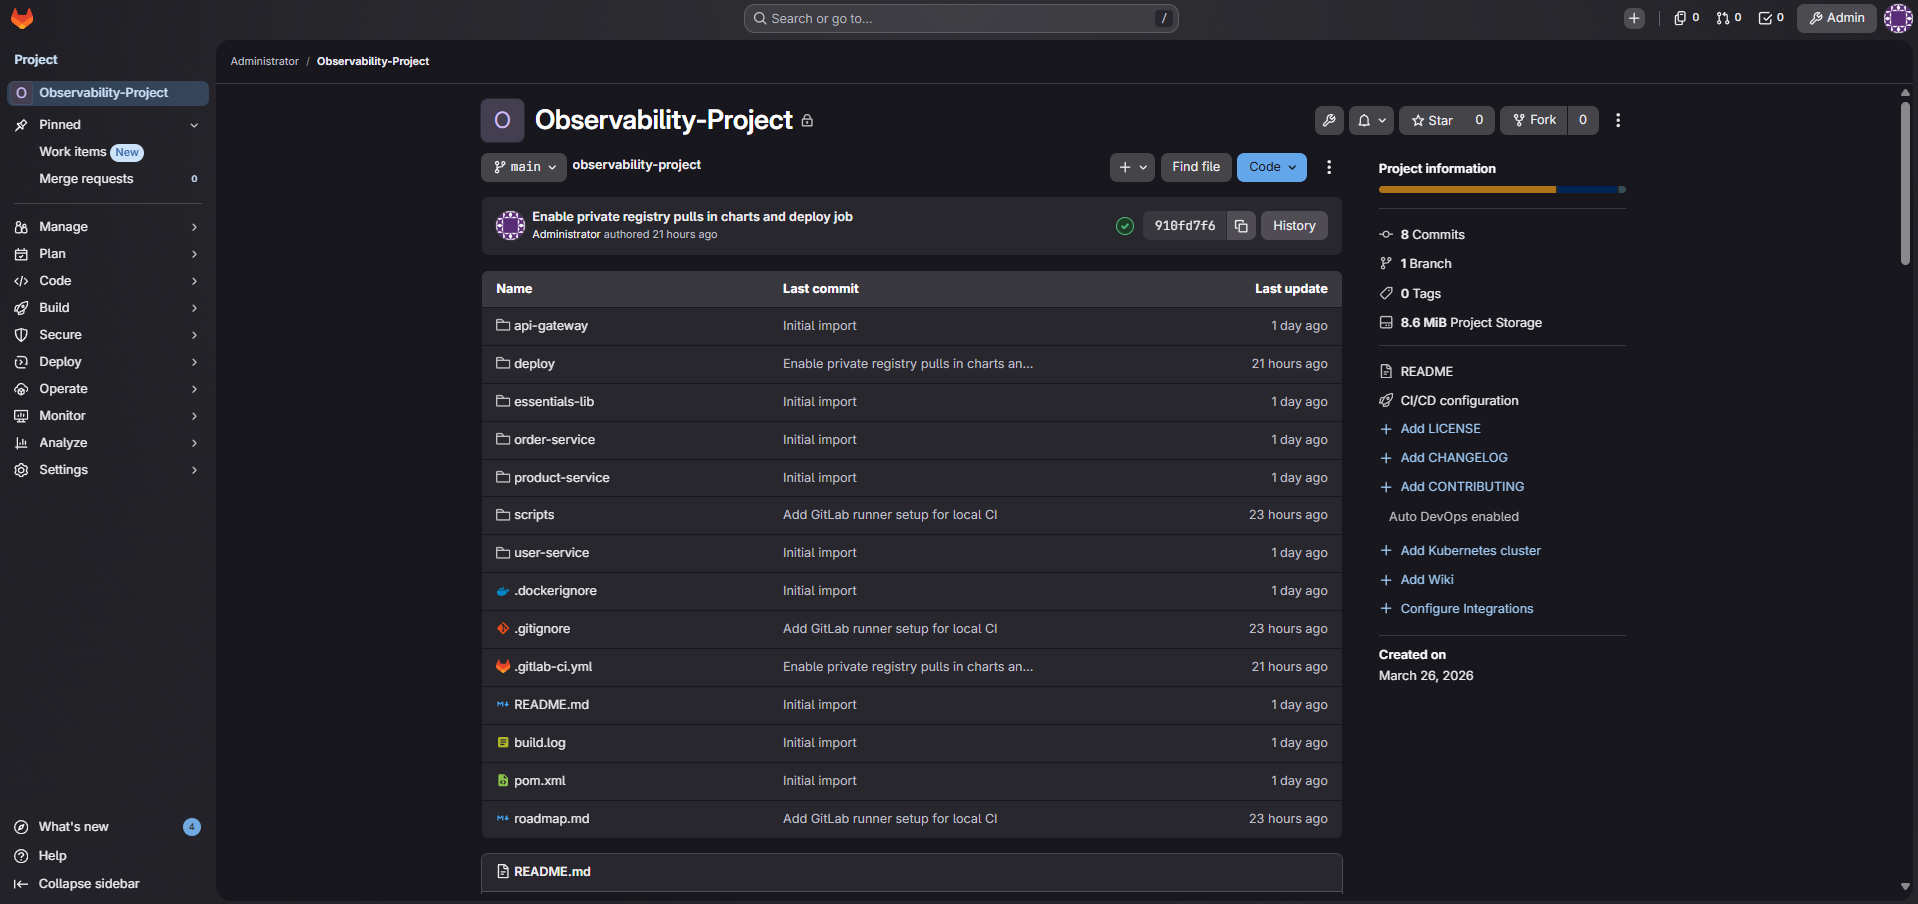
\includegraphics[width=\textwidth]{assets/gitlab/50-gitlab-home-project.png}%
}{%
  \fbox{\parbox{0.92\textwidth}{%
  \textbf{Falta la imagen real:} colocar aquí
  \texttt{assets/gitlab/50-gitlab-home-project.png}.%
  }}%
}
\caption{Vista del proyecto \texttt{Observability-Project} en GitLab CE, con el repositorio cargado y preparado para actuar como origen de CI/CD y del Container Registry.}
\label{fig:gitlab-home-project}
\end{figure}

\begin{center}\rule{0.5\linewidth}{0.5pt}\end{center}

\chapter{GitLab Runner en Kubernetes}\label{gitlab-runner-en-kubernetes}

\section{Qué es GitLab Runner y por qué hace falta}\label{quuxe9-es-gitlab-runner-y-por-quuxe9-hace-falta}

GitLab Runner es el agente ejecutor de las pipelines. GitLab almacena el
repositorio, calcula qué jobs deben lanzarse y conserva el estado de la
pipeline, pero no ejecuta los scripts por sí mismo. La ejecución real
recae en el runner.

Esto es importante porque en muchas explicaciones superficiales parece
que GitLab ``hace CI' por sí solo. En realidad GitLab orquesta y
coordina, mientras que el runner trabaja. El runner es la pieza que:

\begin{itemize}
\tightlist
\item
  descarga el código del job
\item
  prepara el entorno de ejecución
\item
  ejecuta comandos como \texttt{mvn test}, \texttt{helm lint} o Kaniko
\item
  devuelve logs, estado y artefactos a GitLab
\end{itemize}

En este laboratorio el runner es imprescindible porque se quería que la
automatización hiciera trabajo real sobre la plataforma: compilar Maven,
lanzar tests, validar charts, construir imágenes, publicarlas en el
registry y desplegarlas de nuevo en Minikube.

\section{Por qué se desplegó el runner dentro de Kubernetes}\label{por-quuxe9-se-despleguxf3-el-runner-dentro-de-kubernetes}

Una vez desplegado GitLab, se decidió no instalar el runner en Windows.
En su lugar, se desplegó GitLab Runner dentro del propio clúster
mediante Helm. Esta decisión tiene varias ventajas:

\begin{itemize}
\tightlist
\item
  mantiene GitLab, el runner y el destino de despliegue dentro del mismo
  entorno técnico
\item
  evita depender del estado del host Windows para ejecutar jobs
\item
  permite que cada job se ejecute en un pod efímero y aislado
\item
  acerca el laboratorio a un patrón cloud-native más realista
\end{itemize}

\section{Por qué hubo que crear primero un runner en GitLab y luego instalar el chart}\label{por-quuxe9-hubo-que-crear-primero-un-runner-en-gitlab-y-luego-instalar-el-chart}

Este paso suele generar confusión y conviene explicarlo con claridad. El
proceso tuvo dos partes diferentes:

\begin{enumerate}
\def\labelenumi{\arabic{enumi}.}
\tightlist
\item
  en la interfaz de GitLab se creó el \emph{runner lógico}, es decir, el
  registro del agente autorizado para ejecutar jobs del proyecto
\item
  después se instaló el chart \texttt{gitlab-runner} en Kubernetes, que
  despliega el proceso real que usa ese token y se conecta a GitLab
\end{enumerate}

En términos simples, la interfaz de GitLab crea la identidad y entrega el
token; el chart de Helm despliega el agente que consume ese token. Sin
la primera parte, el pod no sabría cómo autenticarse. Sin la segunda,
GitLab tendría un runner definido pero ningún ejecutor real detrás.

Esta distinción es muy útil didácticamente porque separa dos conceptos
que a menudo se mezclan:

\begin{itemize}
\tightlist
\item
  \textbf{definición del runner en GitLab}: autorización, visibilidad en
  la UI, token y pertenencia al proyecto
\item
  \textbf{proceso GitLab Runner desplegado por Helm}: pod real que
  pregunta por jobs, crea pods efímeros y ejecuta scripts
\end{itemize}

Dicho de otra forma: en la web se dio de alta al ``trabajador';
en Kubernetes se desplegó al ``trabajador de verdad' que podía
ponerse a ejecutar tareas.

\section{Configuración relevante del runner}\label{configuraciuxf3n-relevante-del-runner}

El runner quedó definido en \texttt{deploy/gitlab-runner/values.yaml}
con parámetros importantes como estos:

\begin{PlainCode}
gitlabUrl: http://gitlab-webservice-default.gitlab.svc.cluster.local:8181/

runners:
  config: |
    [[runners]]
      clone_url = "http://gitlab-webservice-default.gitlab.svc.cluster.local:8181"
      request_concurrency = 2
      [runners.kubernetes]
        namespace = "gitlab-runner"
        service_account = "gitlab-runner"
        image = "alpine:3.20"
        privileged = true
\end{PlainCode}

\section{Qué resuelve cada parámetro importante}\label{quuxe9-resuelve-cada-paruxe1metro-importante}

\begin{itemize}
\tightlist
\item
  \texttt{gitlabUrl} apunta al servicio interno de GitLab dentro del
  clúster, no a la URL humana del navegador.
\item
  \texttt{clone\_url} fuerza el clonado del repositorio mediante una URL
  alcanzable desde los pods del runner.
\item
  \texttt{service\_account} permite aplicar RBAC específico a los jobs.
\item
  \texttt{privileged = true} habilita escenarios de build más complejos y
  la ejecución de jobs que interactúan con contenedores.
\end{itemize}

\section{Qué es exactamente un runner}\label{quuxe9-es-exactamente-un-runner}

Para un lector conviene describir el flujo completo:

\begin{enumerate}
\def\labelenumi{\arabic{enumi}.}
\tightlist
\item
  GitLab detecta un commit y genera un pipeline
\item
  el runner consulta si hay trabajo pendiente
\item
  el runner reclama un job concreto
\item
  el runner crea un pod efímero en Kubernetes para ejecutarlo
\item
  el pod ejecuta el script del job y devuelve el resultado a GitLab
\end{enumerate}

Esta sección solapa mucho con la definición general de runner, así que se
ha dejado una sola explicación consolidada para evitar redundancia.

\section{Por qué se usó URL interna del servicio GitLab}\label{por-quuxe9-se-usuxf3-url-interna-del-servicio-gitlab}

Uno de los aprendizajes más importantes de esta fase fue diferenciar dos
tipos de URL:

{\small
\begin{tabular}{p{0.19\linewidth}p{0.46\linewidth}p{0.23\linewidth}}
\toprule
\textbf{Tipo de URL} & \textbf{Ejemplo} & \textbf{Quién la usa} \\
\midrule
URL humana & \url{https://gitlab.192.168.49.2.nip.io:8443} & navegador desde Windows \\
URL interna de clúster & \url{http://gitlab-webservice-default.gitlab.svc.cluster.local:8181/} & runner y pods dentro de Kubernetes \\
\bottomrule
\end{tabular}
}

La distinción es crítica: una URL útil para el usuario no tiene por qué
ser válida para componentes internos del clúster. Esa fue la razón por
la que el runner se configuró con direcciones internas para registrarse y
clonar.

\section{Qué problema resolvió \texttt{clone\_url}}\label{quuxe9-problema-resolviuxf3-clone-url}

En la práctica, el runner no solo necesitaba registrarse, sino también
clonar el repositorio. Sin \texttt{clone\_url}, los jobs intentaban usar
la URL pública del proyecto y fallaban desde dentro del clúster. El
parámetro resolvió exactamente ese salto entre red humana y red interna.

\section{Estado operativo del runner}\label{estado-operativo-del-runner}

La captura siguiente muestra el runner ya registrado, asociado al
proyecto y en estado operativo, lo que demuestra que GitLab y el agente
ejecutor quedaron correctamente enlazados.

\begin{figure}[H]
\centering
\IfFileExists{assets/gitlab/51-gitlab-runner-online.png}{%
  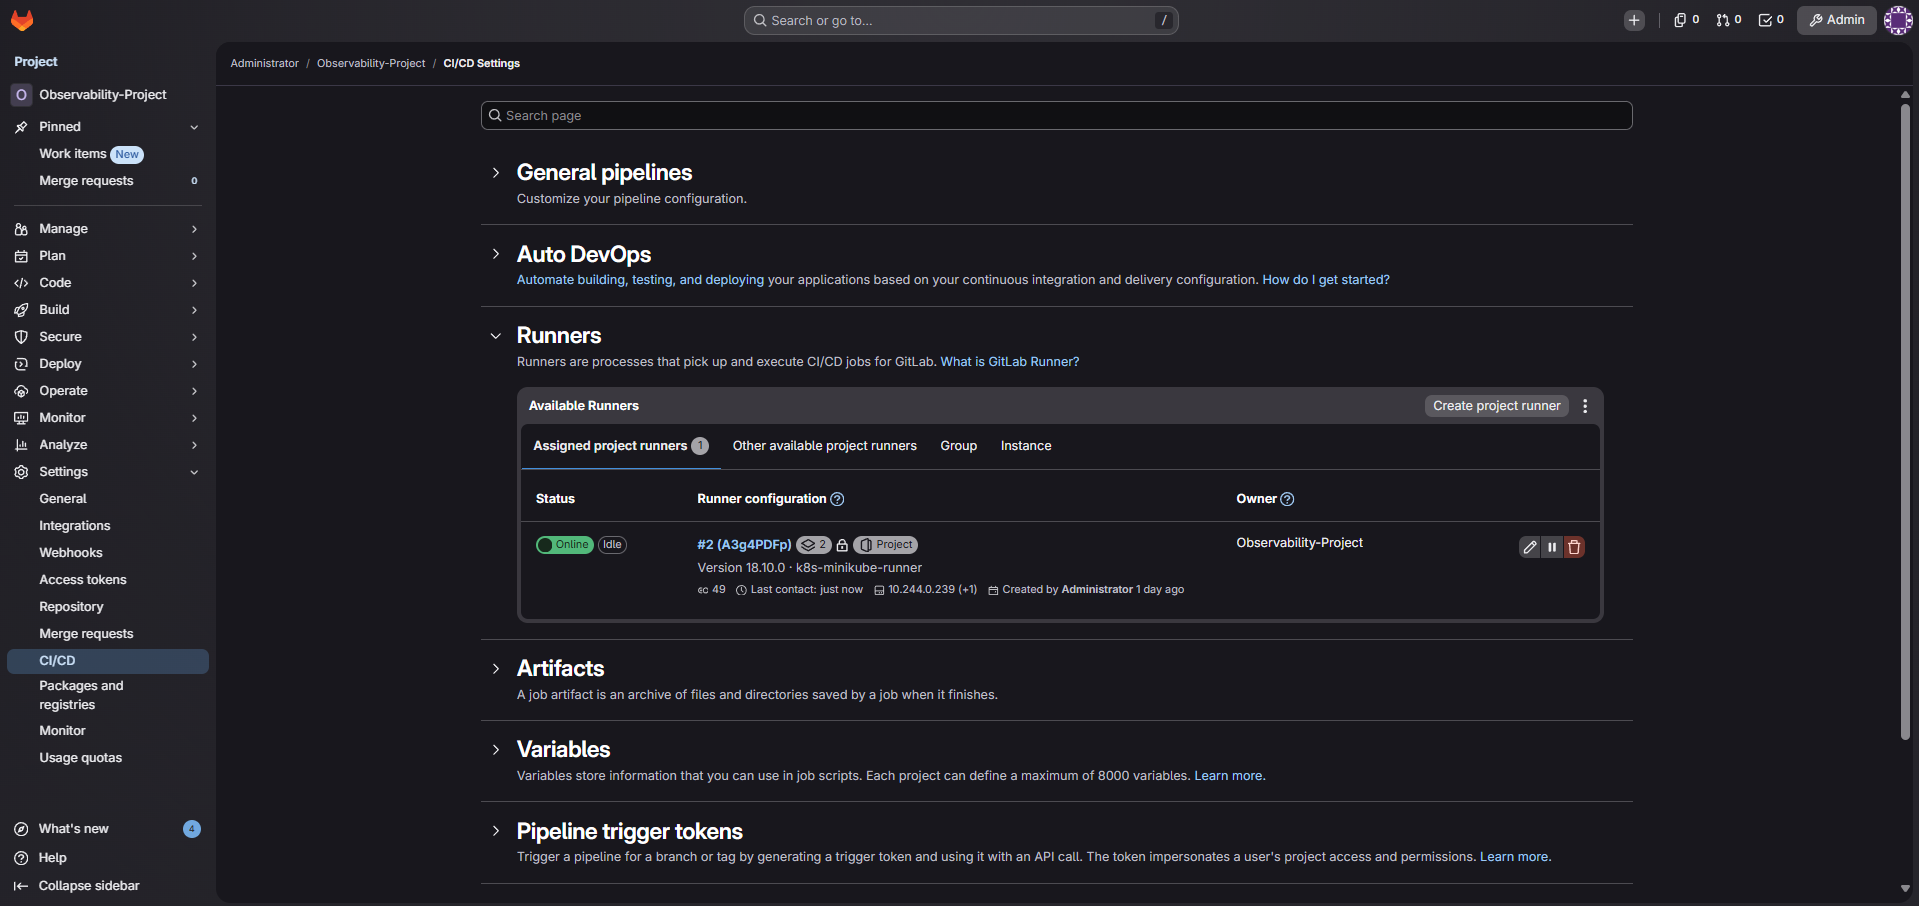
\includegraphics[width=\textwidth]{assets/gitlab/51-gitlab-runner-online.png}%
}{%
  \fbox{\parbox{0.92\textwidth}{%
  \textbf{Falta la imagen real:} colocar aquí
  \texttt{assets/gitlab/51-gitlab-runner-online.png}.%
  }}%
}
\caption{Runner del proyecto en estado \texttt{online} y \texttt{idle}, asociado a \texttt{Observability-Project} tras su registro en GitLab y su despliegue real en Kubernetes mediante Helm.}
\label{fig:gitlab-runner-online}
\end{figure}

\begin{center}\rule{0.5\linewidth}{0.5pt}\end{center}

\chapter{Pipeline CI con GitLab}\label{pipeline-ci-con-gitlab}

\section{Qué es un pipeline y qué significan CI y CD}\label{quuxe9-es-un-pipeline-y-quuxe9-significan-ci-y-cd}

Un \emph{pipeline} es una cadena ordenada de jobs automatizados que se
ejecutan como respuesta a un evento, normalmente un commit o un merge.
Cada job valida, construye o despliega una parte del sistema. En este
proyecto la pipeline se diseñó para reflejar el ciclo de vida completo
que interesa en un laboratorio DevOps: comprobar que el código compila,
que pasa pruebas, que los charts son válidos, que las imágenes se
construyen y que el despliegue puede realizarse con trazabilidad.

Conviene entender el pipeline como una línea de montaje software. El
commit entra por un extremo y, si todo va bien, sale por el otro lado
convertido en un artefacto validado y desplegable. Cada stage cumple una
función de control de calidad: si falla \texttt{build}, el código no
compila; si falla \texttt{test}, el comportamiento no es fiable; si
falla \texttt{validate}, la infraestructura declarativa no está bien
expresada; si falla \texttt{image}, no existe contenedor publicable; si
falla \texttt{deploy}, el clúster no ha aceptado la nueva revisión.

CI significa \emph{Continuous Integration}. Su objetivo es integrar
cambios pequeños de forma frecuente y validarlos automáticamente para
detectar errores cuanto antes. CD puede interpretarse en dos niveles:

\begin{itemize}
\tightlist
\item
  \emph{Continuous Delivery}: el sistema queda siempre en un estado
desplegable y el despliegue puede lanzarse de forma controlada
\item
  \emph{Continuous Deployment}: el despliegue se realiza automáticamente
sin intervención manual
\end{itemize}

En este laboratorio se implementó una CI completa y una CD controlada:
la parte de build, test, empaquetado e imagen se ejecuta de forma
automática, mientras que el despliegue en Minikube se dejó manual para
mantener el control didáctico del proceso. Esto tiene sentido porque el
objetivo del laboratorio no era maximizar automatización ciega, sino
entender qué hace cada pieza del flujo.

\section{Para qué sirve la pipeline en este laboratorio}\label{para-quuxe9-sirve-la-pipeline-en-este-laboratorio}

La pipeline no se añadió solo para poder decir que existe CI/CD. Se
utilizó para resolver necesidades concretas:

\begin{itemize}
\tightlist
\item
  detectar errores de compilación antes del despliegue
\item
  ejecutar tests con una base de datos efímera y realista
\item
  validar que los charts Helm renderizan correctamente
\item
  construir imágenes versionadas por commit
\item
  publicar esas imágenes en el Container Registry
\item
  desplegar exactamente el artefacto construido por la pipeline
\end{itemize}

El valor pedagógico está en que el commit deja de ser solo código fuente
y pasa a convertirse en una unidad trazable de entrega.

\section{Estructura de stages}\label{estructura-de-stages}

La pipeline terminó evolucionando a:

\begin{YamlCode}
stages:
  - build
  - test
  - package
  - validate
  - image
  - deploy
\end{YamlCode}

Esta secuencia refleja el orden lógico de madurez del proceso: primero
se valida el código, después su empaquetado y configuración, luego la
construcción de imágenes y finalmente el despliegue.

\section{Qué son Testcontainers y por qué se usaron}\label{quuxe9-son-testcontainers-y-por-quuxe9-se-usaron}

Testcontainers es una librería de testing que permite arrancar
contenedores reales durante la ejecución de pruebas automatizadas. En
lugar de ejecutar los tests contra H2 o contra mocks excesivamente
artificiales, los servicios pueden validarse contra una base PostgreSQL
efímera levantada específicamente para el test.

Esto es importante porque acerca el comportamiento del test al entorno
real. En el laboratorio se usó para que las pruebas de persistencia y
migraciones se ejecutaran contra PostgreSQL y no contra una base
simplificada con diferencias semánticas. Para un proyecto con Flyway,
JPA y consultas reales, esta diferencia es crítica: un test verde sobre
H2 puede ocultar errores que sí aparecerán contra PostgreSQL.

La idea operativa es sencilla. El propio test declara una URL especial y
el driver de Testcontainers interpreta esa URL como una instrucción para
levantar un contenedor temporal:

\begin{PropertiesCode}
spring.datasource.url=jdbc:tc:postgresql:16-alpine:///userdb
spring.datasource.driver-class-name=org.testcontainers.jdbc.ContainerDatabaseDriver
spring.datasource.username=test
spring.datasource.password=test
\end{PropertiesCode}

A partir de ahí, el ciclo es el siguiente:

\begin{enumerate}
\def\labelenumi{\arabic{enumi}.}
\tightlist
\item
  comienza el test
\item
  Testcontainers levanta un PostgreSQL efímero en Docker
\item
  Spring Boot arranca contra esa base real
\item
  Flyway aplica migraciones
\item
  el test ejecuta repositorios, servicios o endpoints
\item
  al terminar, el contenedor se destruye
\end{enumerate}

Eso transforma la calidad de la validación: el test deja de ser una
comprobación superficial y pasa a simular un trozo importante del
runtime real. En cuanto el test necesita Docker para levantar ese
contenedor efímero, la infraestructura de CI también tiene que
adaptarse. Por eso la fase \texttt{test} se ejecuta con
\texttt{docker:dind} en la pipeline.

\section{Fragmento real de la pipeline}\label{fragmento-real-de-la-pipeline}

La parte principal de la pipeline quedó así:

\begin{YamlCode}
stages:
  - build
  - test
  - package
  - validate
  - image
  - deploy

build:
  stage: build
  image: maven:3.9.9-eclipse-temurin-17
  script:
    - mvn -B -ntp -DskipTests clean compile

test:
  stage: test
  image: maven:3.9.9-eclipse-temurin-17
  services:
    - name: docker:27.5.1-dind
      alias: docker
  variables:
    DOCKER_HOST: tcp://docker:2375
    DOCKER_TLS_CERTDIR: ""
\end{YamlCode}

\section{Qué valida cada fase principal}\label{quuxe9-valida-cada-fase-principal}

\begin{itemize}
\tightlist
\item
  \texttt{build}: comprueba que el proyecto compila
\item
  \texttt{test}: ejecuta pruebas automáticas, incluyendo las apoyadas en
  Testcontainers
\item
  \texttt{package}: empaqueta los microservicios como artefactos Java
\item
  \texttt{validate\_helm}: verifica sintaxis y render de los charts Helm
\item
  \texttt{image}: construye y publica imágenes en el registry
\item
  \texttt{deploy}: despliega manualmente el commit versionado en
  Minikube
\end{itemize}

\section{Evidencia visual de la pipeline en verde}\label{evidencia-visual-de-la-pipeline-en-verde}

La siguiente captura muestra la pipeline en estado satisfactorio, con los
jobs principales de validación y despliegue completados. Esta evidencia
es importante porque demuestra que la automatización no se quedó en un
pipeline teórico: compiló, testó, validó charts, construyó imágenes y
ejecutó el despliegue.

\begin{figure}[H]
\centering
\IfFileExists{assets/gitlab/52-gitlab-pipeline-ci-green.png}{%
  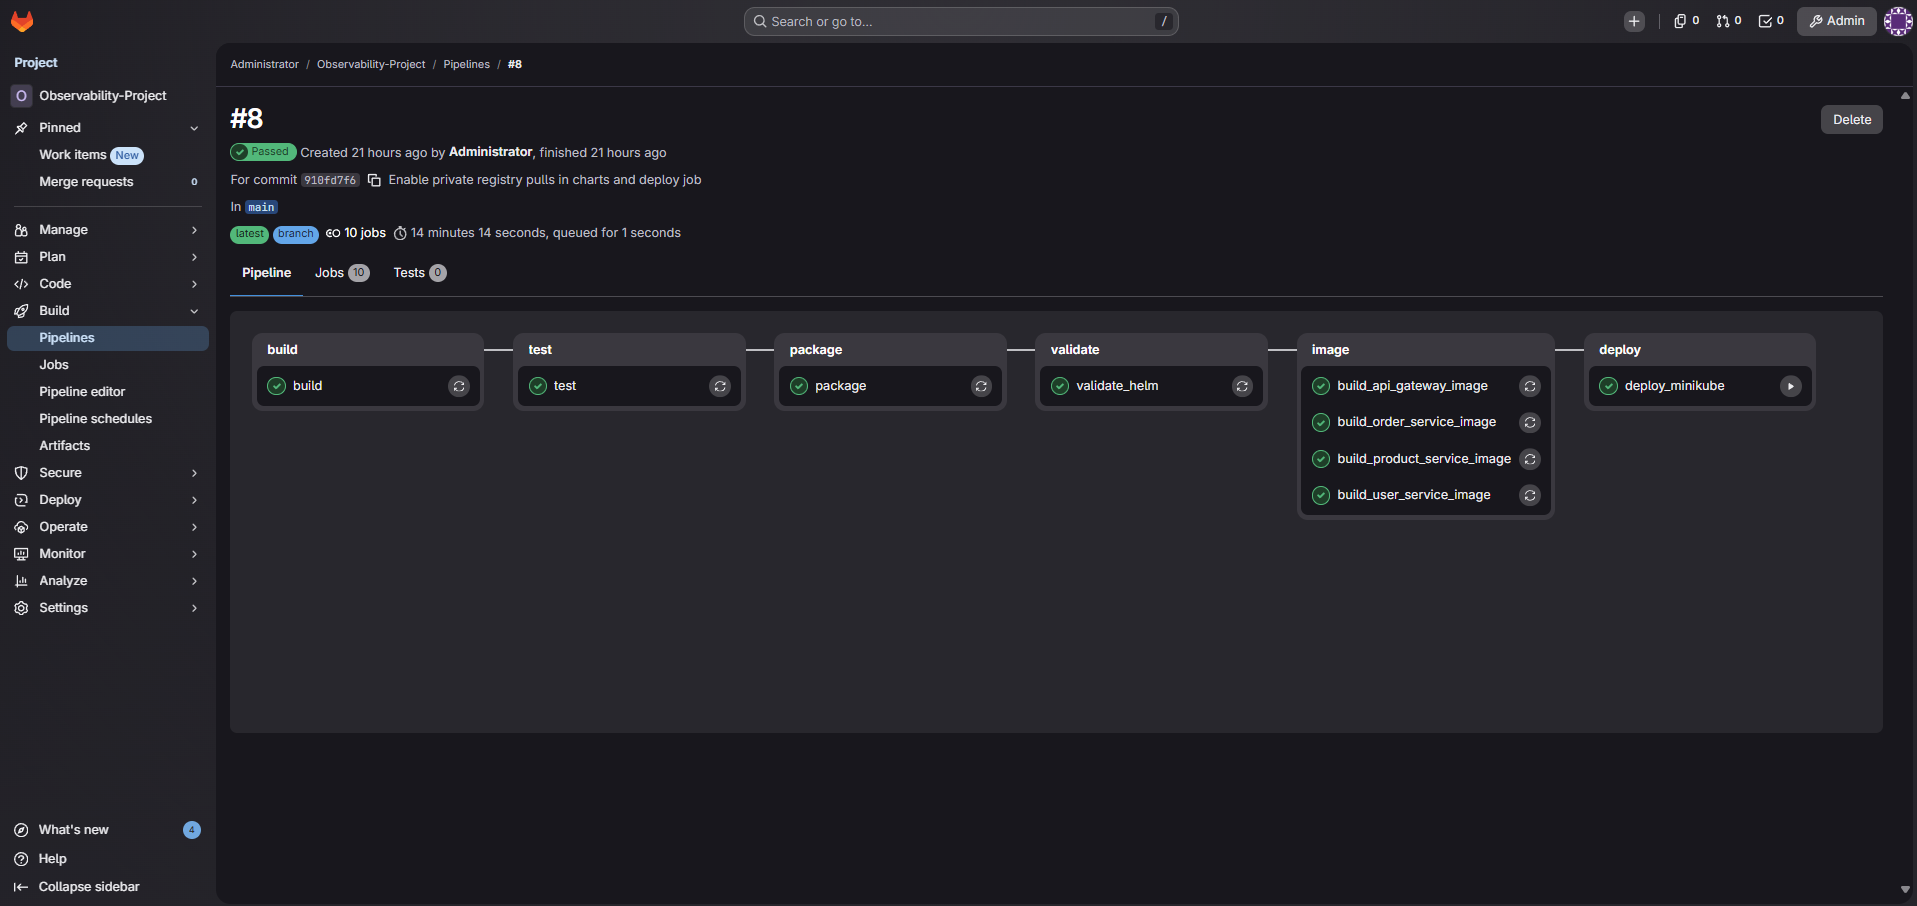
\includegraphics[width=\textwidth]{assets/gitlab/52-gitlab-pipeline-ci-green.png}%
}{%
  \fbox{\parbox{0.92\textwidth}{%
  \textbf{Falta la imagen real:} colocar aquí
  \texttt{assets/gitlab/52-gitlab-pipeline-ci-green.png}.%
  }}%
}
\caption{Pipeline del proyecto en GitLab con los stages de \texttt{build}, \texttt{test}, \texttt{package}, \texttt{validate\_helm}, construcción de imágenes y \texttt{deploy\_minikube} completados correctamente.}
\label{fig:gitlab-pipeline-green}
\end{figure}

\begin{center}\rule{0.5\linewidth}{0.5pt}\end{center}

\chapter{CD real con Container Registry y deploy por
SHA}\label{cd-real-con-container-registry-y-deploy-por-sha}

\section{Qué significa CD en este laboratorio}\label{quuxe9-significa-cd-en-este-laboratorio}

Hasta este punto del informe ya existía una CI completa: el código se
compilaba, se ejecutaban tests, se validaban charts y se obtenía una
pipeline fiable. Sin embargo, todavía faltaba una pregunta clave: \emph{¿cómo
se convierte exactamente un commit en una versión desplegada en el
clúster?}

Ahí entra la parte de CD. En este documento, CD se entiende como
\emph{Continuous Delivery} con despliegue controlado. Es decir, cada
commit que supera la pipeline queda convertido en una imagen versionada
y lista para desplegarse, aunque el paso final de despliegue se mantenga
manual para conservar el control del laboratorio.

La diferencia con la CI es importante:

\begin{itemize}
\tightlist
\item
  la \textbf{CI} responde a la pregunta ``¿el cambio es válido?'
\item
  la \textbf{CD} responde a la pregunta ``¿qué artefacto exacto se
despliega y cómo llega al clúster?'
\end{itemize}

En un entorno profesional, esta segunda parte es crítica. No basta con
que el código compile; hace falta saber qué imagen concreta se ha
publicado, qué tag la identifica, qué pipeline la generó y qué
Deployment la está ejecutando.

\section{De imágenes locales a registry
privado}\label{de-imuxe1genes-locales-a-registry-privado}

Al principio el laboratorio funcionaba con imágenes construidas dentro
de Minikube. Esto era útil para iterar rápido, pero no representaba una
cadena de despliegue real. El siguiente paso fue usar el GitLab
Container Registry como fuente oficial de imágenes.

Ese cambio modifica por completo el modelo operativo. En lugar de que el
clúster use una imagen ``que ya estaba allí', el proceso pasa a ser:

\begin{enumerate}
\def\labelenumi{\arabic{enumi}.}
\tightlist
\item
  GitLab Runner construye la imagen
\item
  la imagen se publica en el registry del proyecto
\item
  la imagen recibe uno o más tags
\item
  el job de despliegue le dice a Helm qué repositorio y qué tag usar
\item
  Kubernetes descarga exactamente esa imagen desde el registry
\end{enumerate}

Este punto es fundamental porque introduce trazabilidad real entre código
y runtime. El commit deja de ser un cambio abstracto en Git y pasa a
quedar materializado como una imagen concreta almacenada en un registry.

\section{Qué es un Container Registry y cómo
funciona}\label{quuxe9-es-un-container-registry-y-cuxf3mo-funciona}

Un \emph{Container Registry} es un servicio especializado en almacenar y
servir imágenes de contenedor. Si GitLab actúa como repositorio del
código fuente, el registry actúa como repositorio de las imágenes ya
construidas.

El paralelismo didáctico es útil:

\begin{itemize}
\tightlist
\item
  Git conserva commits, ramas y tags de código
\item
  el registry conserva repositorios de imágenes y sus tags
\end{itemize}

Cada microservicio del laboratorio termina teniendo su propio repositorio
de imagen dentro del registry, por ejemplo:

\begin{PlainCode}
registry.192.168.49.2.nip.io/root/observability-project/api-gateway
registry.192.168.49.2.nip.io/root/observability-project/user-service
registry.192.168.49.2.nip.io/root/observability-project/product-service
registry.192.168.49.2.nip.io/root/observability-project/order-service
\end{PlainCode}

Sobre cada uno de esos repositorios pueden existir varios tags. Un tag
es simplemente un nombre legible que apunta a una imagen concreta. En
este laboratorio se usaron dos ideas de tag:

\begin{itemize}
\tightlist
\item
  un tag mutable como \texttt{main}, útil para inspección manual
\item
  un tag inmutable basado en el commit, por ejemplo
  \texttt{910fd7f6}, útil para despliegue trazable
\end{itemize}

\section{Cómo se generan los tags y por qué se usa el SHA del commit}\label{cuxf3mo-se-generan-los-tags-y-por-quuxe9-se-usa-el-sha-del-commit}

El objetivo no era solo construir imágenes, sino poder responder a esta
pregunta: \emph{¿qué versión exacta está corriendo en Kubernetes?}

Para resolverlo, cada build publica la imagen con el valor de
\texttt{CI\_COMMIT\_SHORT\_SHA}. Así, si el commit actual es
\texttt{910fd7f6}, la imagen generada queda así:

\begin{PlainCode}
registry.192.168.49.2.nip.io/root/observability-project/user-service:910fd7f6
\end{PlainCode}

Esto tiene varias ventajas:

\begin{itemize}
\tightlist
\item
  el tag es estable e inmutable
\item
  se puede relacionar directamente con el commit de Git
\item
  el despliegue deja una huella fácil de auditar
\item
  un rollback es más simple porque basta con volver a desplegar un SHA
  anterior
\end{itemize}

En otras palabras, el tag por SHA convierte la imagen en una pieza
versionada con semántica operativa real.

\section{Build de imágenes con
Kaniko}\label{build-de-imuxe1genes-con-kaniko}

Para construir imágenes dentro del clúster se eligió Kaniko. La razón
principal es que encaja mejor que Docker-in-Docker en un runner
Kubernetes. Kaniko puede construir imágenes a partir de un
\texttt{Dockerfile} y publicarlas en un registry sin necesitar un daemon
Docker tradicional dentro del job.

Ejemplo simplificado del template de build:

\begin{YamlCode}
.build_image_template:
  stage: image
  image:
    name: gcr.io/kaniko-project/executor:v1.23.2-debug
    entrypoint: [""]
  script:
    - mkdir -p /kaniko/.docker
    - printf '{"auths":{"%s":{"username":"%s","password":"%s"}}}' "$CI_REGISTRY" "$CI_REGISTRY_USER" "$CI_REGISTRY_PASSWORD" > /kaniko/.docker/config.json
    - /kaniko/executor \
      --context "${CI_PROJECT_DIR}" \
      --dockerfile "${CI_PROJECT_DIR}/${SERVICE}/Dockerfile" \
      --destination "${CI_REGISTRY_IMAGE}/${SERVICE}:${CI_COMMIT_SHORT_SHA}" \
      --destination "${CI_REGISTRY_IMAGE}/${SERVICE}:main"
\end{YamlCode}

El job toma el código fuente, ejecuta el \texttt{Dockerfile}, construye
la imagen y la empuja al registry con dos destinos. El más importante de
cara al despliegue es el SHA del commit.

\section{Autenticación contra el registry desde
CI}\label{autenticaciuxf3n-contra-el-registry-desde-ci}

Kaniko necesita autenticarse para hacer \texttt{push} al registry. Para
ello se genera un \texttt{config.json} de Docker dentro del job:

\begin{BashCode}
- mkdir -p /kaniko/.docker
- printf '{"auths":{"%s":{"username":"%s","password":"%s"}}}' "$CI_REGISTRY" "$CI_REGISTRY_USER" "$CI_REGISTRY_PASSWORD" > /kaniko/.docker/config.json
\end{BashCode}

\section{Qué representa este
fragmento}\label{quuxe9-representa-este-fragmento}

\begin{itemize}
\tightlist
\item
  \texttt{CI\_REGISTRY}: host del GitLab Container Registry
\item
  \texttt{CI\_REGISTRY\_USER} y \texttt{CI\_REGISTRY\_PASSWORD}:
  credenciales inyectadas por GitLab CI
\item
  \texttt{/kaniko/.docker/config.json}: ubicación que Kaniko espera para
  autenticarse
\end{itemize}

Este fragmento traduce una idea muy simple: el job necesita credenciales
válidas para poder publicar imágenes. Si esta autenticación falla, la
pipeline puede compilar y testear, pero se rompe exactamente en el salto
entre artefacto lógico e imagen distribuible.

\section{Autenticación contra el registry desde
Kubernetes}\label{autenticaciuxf3n-contra-el-registry-desde-kubernetes}

Una vez publicada la imagen, el clúster también necesita autenticarse
para hacer \texttt{pull}. Para eso se usa un \texttt{imagePullSecret},
que conceptualmente responde a esta idea:

\begin{PlainCode}
Kubernetes no puede descargar una imagen privada si no conoce credenciales válidas para el registry.
\end{PlainCode}

Por eso en los charts se añadió soporte a \texttt{image.pullSecrets}, y
en el namespace de despliegue se creó un secret del tipo
\texttt{docker-registry}.

\begin{YamlCode}
image:
  repository: mercadona/api-gateway
  tag: 0.0.1-SNAPSHOT
  pullPolicy: IfNotPresent
  pullSecrets: []
\end{YamlCode}

Y en el \texttt{Deployment}:

\begin{YamlCode}
{{- with .Values.image.pullSecrets }}
imagePullSecrets:
{{ toYaml . | indent 8 }}
{{- end }}
\end{YamlCode}

Este cambio parece pequeño, pero conceptualmente es enorme. Es el punto
en el que la infraestructura declarativa del chart aprende a consumir
imágenes privadas provenientes del sistema de CI/CD.

\section{Cómo se despliega realmente una imagen por
SHA}\label{cuxf3mo-se-despliega-realmente-una-imagen-por-sha}

El job \texttt{deploy\_minikube} quedó como job manual. Es una decisión
sensata para laboratorio porque evita despliegues automáticos
accidentales y permite validar primero el artefacto construido.

Ejemplo simplificado:

\begin{BashCode}
helm upgrade --install user-service deploy/helm/user-service \
  --namespace default \
  -f deploy/environments/minikube/user-service-values.yaml \
  --set image.repository="${CI_REGISTRY_IMAGE}/user-service" \
  --set image.tag="${CI_COMMIT_SHORT_SHA}"
\end{BashCode}

Este fragmento hace dos cosas muy importantes:

\begin{itemize}
\tightlist
\item
  sustituye el repositorio de imagen del chart por el repositorio real
  del GitLab Container Registry
\item
  sustituye el tag fijo por el SHA del commit que acaba de pasar la
  pipeline
\end{itemize}

El efecto práctico es que Kubernetes no despliega ``la última
imagen local', sino una imagen inmutable asociada a un commit concreto.

\section{Ejemplos de resultado que produce este flujo}\label{ejemplos-de-resultado-que-produce-este-flujo}

Si el commit activo es \texttt{910fd7f6}, dos salidas representativas del
sistema serían estas:

\begin{PlainCode}
registry.192.168.49.2.nip.io/root/observability-project/user-service:910fd7f6
registry.192.168.49.2.nip.io/root/observability-project/order-service:910fd7f6
\end{PlainCode}

Y en Kubernetes, el Deployment puede quedar reflejado así:

\begin{PlainCode}
NAME           IMAGE
user-service   registry.192.168.49.2.nip.io/root/observability-project/user-service:910fd7f6
\end{PlainCode}

Esta es la demostración más clara de CD real: el commit, la pipeline, la
imagen y el deployment quedan unidos por el mismo identificador.

\section{Problemas reales de esta
fase}\label{problemas-reales-de-esta-fase}

Esta parte del proyecto fue especialmente rica en troubleshooting. Entre
los problemas resueltos destacan:

\begin{itemize}
\tightlist
\item
  errores al construir el \texttt{config.json} de Kaniko
\item
  autenticación del registry contra GitLab web
\item
  resolución DNS incorrecta dentro del clúster
\item
  necesidad de confiar en la CA del registry desde el nodo Minikube
\item
  pods bloqueados en \texttt{ErrImageNeverPull}
\end{itemize}

Este bloque es muy valioso en una memoria didáctica porque enseña que el
CD real tiene varias capas:

\begin{enumerate}
\def\labelenumi{\arabic{enumi}.}
\tightlist
\item
  construir la imagen\\
\item
  empujarla al registry\\
\item
  permitir que Kubernetes pueda descargarla\\
\item
  conseguir que el deployment haga rollout correctamente
\end{enumerate}

\section{Evidencias visuales recomendadas y cómo obtenerlas}\label{evidencias-visuales-recomendadas-y-cuxf3mo-obtenerlas}

Para documentar esta fase de forma convincente se han incluido dos
pruebas complementarias: una evidencia visual del Container Registry y
una evidencia textual del Deployment final consumido por Kubernetes.

\subsection*{Container Registry del proyecto}

La siguiente captura muestra uno de los repositorios de imagen del
proyecto dentro del GitLab Container Registry. En ella se aprecia que la
pipeline no publica una única imagen genérica, sino varios tags
asociados a la evolución del proyecto, incluyendo tags por SHA y el tag
\texttt{main}.

\begin{figure}[H]
\centering
\IfFileExists{assets/gitlab/54-gitlab-container-registry.png}{%
  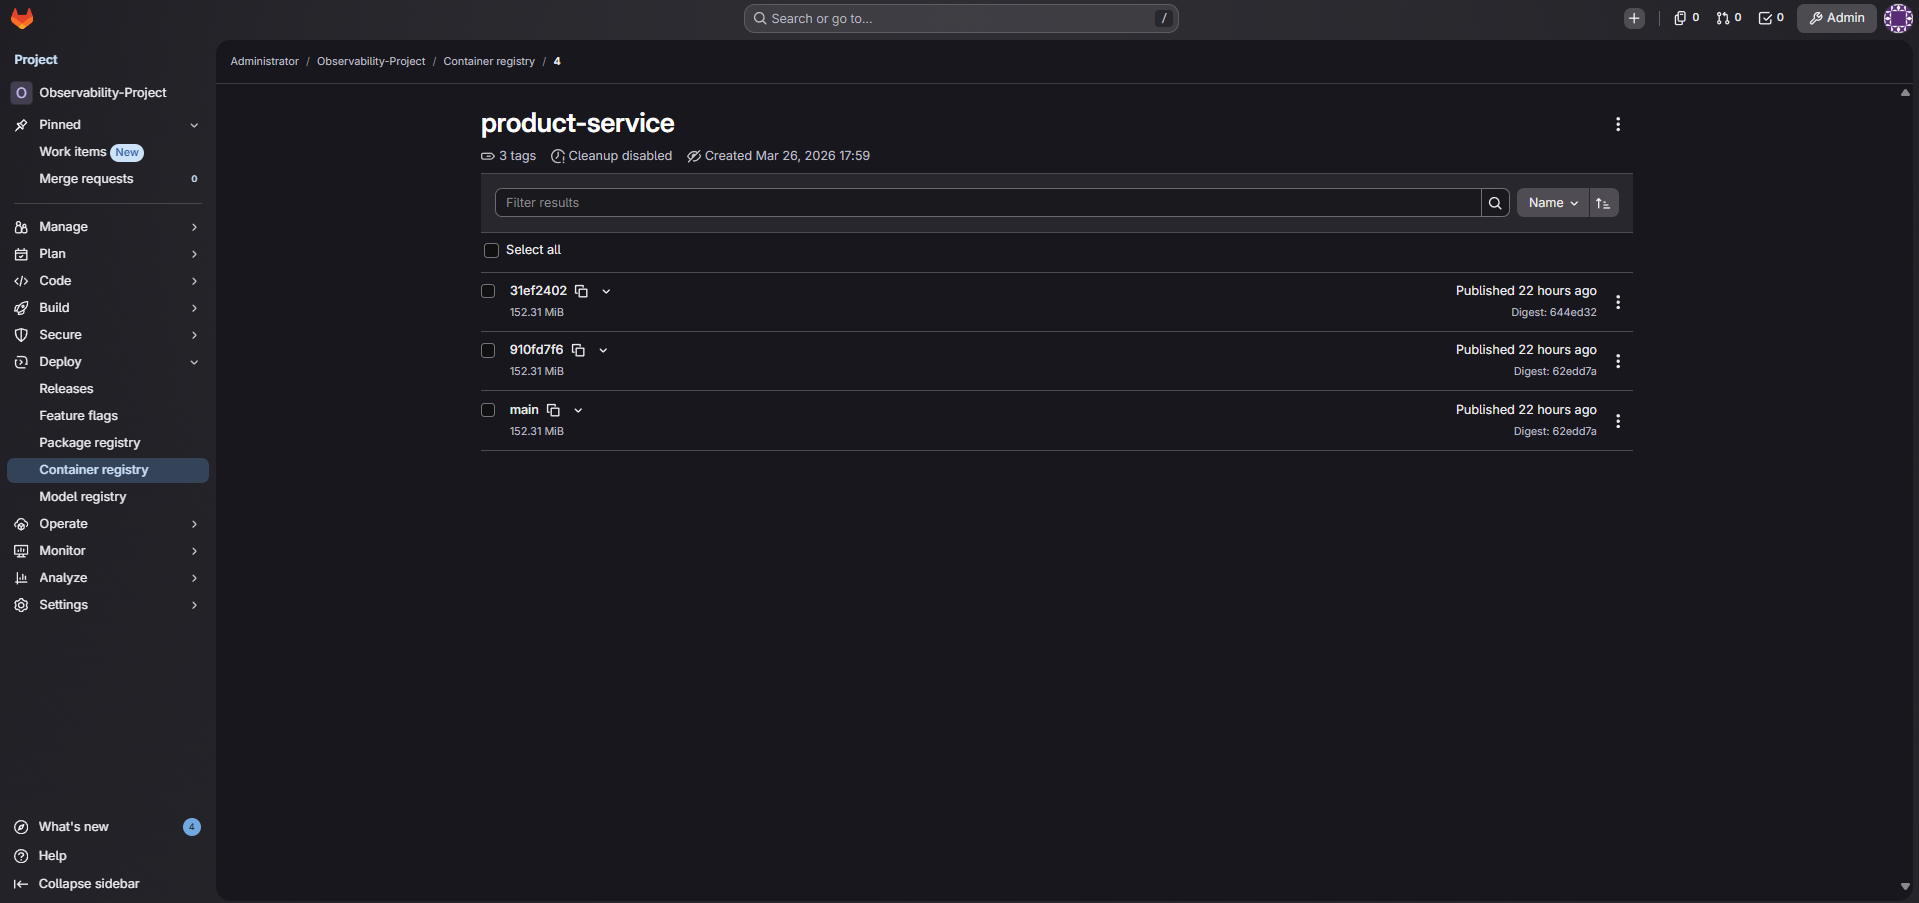
\includegraphics[width=\textwidth]{assets/gitlab/54-gitlab-container-registry.png}%
}{%
  \fbox{\parbox{0.92\textwidth}{%
  \textbf{Falta la imagen real:} colocar aquí
  \texttt{assets/gitlab/54-gitlab-container-registry.png}.%
  }}%
}
\caption{Repositorio de imágenes en el GitLab Container Registry, con varios tags publicados por la pipeline para un microservicio del laboratorio.}
\label{fig:gitlab-container-registry}
\end{figure}

Esta vista es relevante porque demuestra que la CD no termina en el
build. La pipeline construye una imagen, la identifica con tags
significativos y la deja disponible para que el clúster la consuma.

\subsection*{Deployment final consumido por Kubernetes}

En lugar de añadir una segunda captura, se incluye la salida de terminal
obtenida al consultar el Deployment del \texttt{user-service}. En esta
memoria se ha normalizado el prefijo del repositorio a
\texttt{observability} para mantener una nomenclatura homogénea en el
texto del documento.

\begin{PowerShellCode}
PS C:\Users\Usuario\Desktop\Personal\Proyectos\Devops\Observability Lab> kubectl get deployment user-service -n default -o custom-columns=NAME:.metadata.name,IMAGE:.spec.template.spec.containers[0].image
NAME           IMAGE
user-service   observability/user-service:0.0.1-SNAPSHOT
\end{PowerShellCode}

Esta evidencia sirve para explicar una idea muy importante: el estado
final del Deployment puede consultarse directamente desde Kubernetes, y
esa consulta permite verificar qué imagen exacta está declarada en el
runtime. En una versión completamente orientada a SHA, esta misma salida
podría mostrar un tag como \texttt{910fd7f6}; en cualquier caso, el
principio es el mismo: el Deployment referencia una imagen concreta y
visible para el operador.

\begin{center}\rule{0.5\linewidth}{0.5pt}\end{center}

\chapter{Decisiones de diseño y
trade-offs}\label{decisiones-de-diseuxf1o-y-trade-offs}

Esta sección es importante porque transforma el documento de una simple
narración de hechos en una memoria con criterio técnico. No basta con
decir qué se hizo; también conviene explicar por qué se eligió una
alternativa y no otra.

\section{Microservicios acoplados por HTTP frente a servicios
aislados}\label{microservicios-acoplados-por-http-frente-a-servicios-aislados}

Se eligió un flujo con dependencias HTTP reales entre servicios. La
razón no fue puramente funcional, sino observacional.

{\def\LTcaptype{none} % do not increment counter
\begin{longtable}[]{@{}
  >{\raggedright\arraybackslash}p{(\linewidth - 4\tabcolsep) * \real{0.3333}}
  >{\raggedright\arraybackslash}p{(\linewidth - 4\tabcolsep) * \real{0.3333}}
  >{\raggedright\arraybackslash}p{(\linewidth - 4\tabcolsep) * \real{0.3333}}@{}}
\toprule\noalign{}
\begin{minipage}[b]{\linewidth}\raggedright
Opción
\end{minipage} & \begin{minipage}[b]{\linewidth}\raggedright
Ventaja
\end{minipage} & \begin{minipage}[b]{\linewidth}\raggedright
Inconveniente
\end{minipage} \\
\midrule\noalign{}
\endhead
\bottomrule\noalign{}
\endlastfoot
Servicios aislados & simplicidad & menos valor para trazas y
correlación \\
Servicios con dependencias HTTP & más realismo y observabilidad
distribuida & más complejidad operativa \\
\end{longtable}
}

En este laboratorio interesaba más el valor didáctico de la segunda
opción.

\section{PostgreSQL único con esquemas frente a méltiples
bases}\label{postgresql-uxfanico-con-esquemas-frente-a-muxe9ltiples-bases}

Se eligió una única instancia PostgreSQL con varios esquemas.

Razones:

\begin{itemize}
\tightlist
\item
  menos consumo de recursos en local
\item
  menos complejidad de operación
\item
  aislamiento lógico suficiente para laboratorio
\end{itemize}

Trade-off:

\begin{itemize}
\tightlist
\item
  no reproduce al cien por cien una separación completa por base de
  datos
\item
  sí reproduce suficientemente bien versionado, migraciones y
  persistencia real
\end{itemize}

\section{Helm frente a manifiestos Kubernetes
sueltos}\label{helm-frente-a-manifiestos-kubernetes-sueltos}

Helm añade una capa más de complejidad que \texttt{kubectl\ apply}, pero
aporta ventajas decisivas:

\begin{itemize}
\tightlist
\item
  parametrización por entorno
\item
  plantillas reutilizables
\item
  despliegues repetibles
\item
  mejor integración con CI/CD
\end{itemize}

Para un proyecto con varios microservicios, Helm es una decisión
razonable incluso en laboratorio.

\section{OpenTelemetry solo para
trazas}\label{opentelemetry-solo-para-trazas}

Aunque OpenTelemetry puede participar en métricas y logs, en este
laboratorio se decidió separar responsabilidades:

\begin{itemize}
\tightlist
\item
  trazas -\textgreater{} OpenTelemetry
\item
  métricas -\textgreater{} Prometheus
\item
  logs -\textgreater{} ECS JSON + Filebeat + Elasticsearch
\end{itemize}

La razón es didáctica y operativa:

\begin{itemize}
\tightlist
\item
  simplifica el modelo mental
\item
  evita duplicidad de señales
\item
  permite enseñar mejor qué backend resuelve cada problema
\end{itemize}

Esta decisión conviene explicarla con más detalle porque, a primera
vista, podría parecer que el laboratorio está renunciando a una parte
importante de OpenTelemetry. En realidad, lo que se hizo fue elegir un
reparto de responsabilidades muy explícito para que cada señal
observacional tuviera un camino fácil de razonar.

\subsection{Qué significa exactamente separar señales}
\label{que-significa-exactamente-separar-senales}

En este laboratorio una misma operación de negocio genera varios tipos de
evidencia, pero cada evidencia toma un camino distinto porque responde a
preguntas distintas. Si un usuario crea un pedido a través del gateway,
lo que ocurre en segundo plano es algo parecido a esto:

\begin{itemize}
\tightlist
\item
  la petición HTTP genera una \emph{traza} y varios \emph{spans}, por lo
  que esa señal se envía mediante OpenTelemetry y OTLP al Collector y,
  desde ahí, a Jaeger
\item
  esa misma petición incrementa contadores y latencias agregadas, por lo
  que esa señal se expone en \texttt{/actuator/prometheus} y Prometheus la
  obtiene por \emph{scraping}
\item
  el procesamiento interno de la petición escribe eventos estructurados
  en consola en formato ECS JSON, y Filebeat los reenvía a Elasticsearch
\end{itemize}

Esto permite contestar tres tipos de preguntas con tres herramientas
especializadas:

\begin{itemize}
\tightlist
\item
  \textbf{trazas}: ``¿qué servicios participaron y en qué orden?''
\item
  \textbf{métricas}: ``¿cuánto tarda de media y cuántas veces ocurre?''
\item
  \textbf{logs}: ``¿qué pasó exactamente y con qué contexto?''
\end{itemize}

Ese reparto transforma el comportamiento del sistema de forma muy clara.
El microservicio deja de verse como una caja negra que solo devuelve una
respuesta HTTP y pasa a comportarse como una fuente de telemetría con
varios planos de observación.

\subsection{Ejemplo práctico de una petición en este modelo}
\label{ejemplo-practico-de-una-peticion-en-este-modelo}

Si el cliente invoca \texttt{POST /api/orders}, el laboratorio obtiene al
menos tres resultados distintos:

\begin{itemize}
\tightlist
\item
  en Jaeger aparece una traza donde se ve \texttt{api-gateway},
  \texttt{order-service}, \texttt{user-service} y \texttt{product-service}
  con su relación temporal
\item
  en Prometheus aumentan métricas como peticiones por segundo, latencia
  media o errores por servicio
\item
  en Kibana aparecen eventos con \texttt{service.name}, \texttt{log.level},
  \texttt{message} y \texttt{trace\_id}
\end{itemize}

Un ejemplo simplificado del flujo sería:

\begin{PlainCode}
Cliente
  -> api-gateway
  -> order-service
     -> user-service
     -> product-service

Resultados observables:
  trazas -> OTel -> OTel Collector -> Jaeger
  métricas -> /actuator/prometheus -> Prometheus
  logs -> ECS JSON -> Filebeat -> Elasticsearch -> Kibana
\end{PlainCode}

\subsection{Qué se habría podido hacer con OpenTelemetry para más
señales}\label{que-se-habria-podido-hacer-con-opentelemetry-para-mas-senales}

OpenTelemetry no está limitado a trazas. El estándar puede transportar
también métricas y logs. Una arquitectura alternativa habría sido:

\begin{itemize}
\tightlist
\item
  microservicios instrumentados con OpenTelemetry para trazas
\item
  exportación de métricas también por OTLP hacia un Collector
\item
  el Collector reenviando esas métricas a Prometheus Remote Write, a otro
  backend compatible o incluso a OpenSearch
\item
  logs enriquecidos con atributos OpenTelemetry además del formato JSON
\end{itemize}

Un ejemplo simplificado de exportación OTLP desde Spring Boot sería:

\begin{PropertiesCode}
otel.service.name=order-service
otel.exporter.otlp.endpoint=http://otel-collector.observability.svc.cluster.local:4318
otel.traces.exporter=otlp
otel.metrics.exporter=otlp
otel.logs.exporter=otlp
\end{PropertiesCode}

En ese modelo el microservicio no solo produciría spans, sino que
delegaría en el ecosistema OpenTelemetry la entrega de varias señales. La
ventaja es que la canalización queda más unificada. El inconveniente,
especialmente en un laboratorio didáctico, es que la frontera entre
responsabilidades se vuelve menos evidente.

\subsection{Por qué en este laboratorio no se eligió ese
modelo}\label{por-que-en-este-laboratorio-no-se-eligio-ese-modelo}

Si el objetivo principal del proyecto hubiera sido construir una capa de
telemetría completamente unificada, habría tenido sentido empujar más
señales por OpenTelemetry. Sin embargo, el objetivo principal de este
laboratorio es pedagógico: entender qué problema resuelve cada pieza.

Por eso se buscó que cada backend tuviera un papel muy fácil de
explicar:

\begin{itemize}
\tightlist
\item
  \textbf{Jaeger} recibe trazas distribuidas y permite ver la relación
  temporal entre spans
\item
  \textbf{Prometheus} recoge series temporales y responde bien a
  preguntas agregadas como tasa, error ratio o percentiles
\item
  \textbf{Elasticsearch + Kibana} almacenan y exploran eventos
  estructurados, con filtros por servicio, severidad y \texttt{trace\_id}
\end{itemize}

Este reparto es especialmente útil para perfiles junior porque evita la
sensación de que ``todo entra por el mismo tubo''. En una primera
fase de aprendizaje suele ser más valioso entender bien tres caminos
claros que abstraerlo todo detrás de una canalización única.

\subsection{Qué es OTLP y por qué aparece tanto en OpenTelemetry}
\label{que-es-otlp-y-por-que-aparece-tanto-en-opentelemetry}

OTLP significa \emph{OpenTelemetry Protocol}. Es el protocolo estándar
que define cómo se envían trazas, métricas y logs desde una librería o
un agente hacia un Collector o hacia otro backend compatible.

En la práctica, OTLP es importante porque:

\begin{itemize}
\tightlist
\item
  desacopla la instrumentación del destino final
\item
  permite cambiar el backend sin reescribir la aplicación
\item
  facilita usar un Collector intermedio para enriquecer, filtrar o
  reenviar señales
\end{itemize}

En este laboratorio OTLP se usa sobre todo para spans. El flujo mental
es:

\begin{PlainCode}
microservicio Spring Boot
  -> OpenTelemetry SDK / starter
  -> OTLP
  -> OTel Collector
  -> Jaeger
\end{PlainCode}

Si se decidiera usar OTLP también para métricas o logs, cambiaría el
volumen de señales, la configuración del Collector y la necesidad de
explicar con más detalle procesamiento, batching y exportadores
múltiples.

\subsection{Cómo habría sido una variante con OpenSearch}
\label{como-habria-sido-una-variante-con-opensearch}

Otra alternativa razonable habría sido sustituir Elasticsearch y Kibana
por OpenSearch y OpenSearch Dashboards. Conceptualmente el flujo sería
muy parecido:

\begin{PlainCode}
microservicios -> logs JSON estructurados -> Filebeat / Fluent Bit
-> OpenSearch -> OpenSearch Dashboards
\end{PlainCode}

Incluso podría combinarse con OpenTelemetry de forma más agresiva,
utilizando el Collector para reenviar logs o métricas hacia un backend
compatible. Un ejemplo conceptual de Collector para varias señales sería:

\begin{YamlCode}
receivers:
  otlp:
    protocols:
      grpc: {}
      http: {}

exporters:
  otlp/jaeger:
    endpoint: jaeger-collector.observability.svc.cluster.local:4317
    tls:
      insecure: true
  debug: {}

service:
  pipelines:
    traces:
      receivers: [otlp]
      exporters: [otlp/jaeger, debug]
\end{YamlCode}

Si el laboratorio hubiera ido por ese camino, lo que cambiaría de forma
más visible sería:

\begin{itemize}
\tightlist
\item
  el backend de logs y búsqueda
\item
  la interfaz de exploración de eventos
\item
  parte de las plantillas de índices, consultas y dashboards
\item
  la forma de explicar correlación entre logs y trazas
\end{itemize}

En cambio, lo que \emph{no} cambiaría sería la necesidad de producir
logs estructurados de calidad desde la aplicación.

\section{GitLab self-managed dentro de
Minikube}\label{gitlab-self-managed-dentro-de-minikube}

Esta decisión añade complejidad, pero también mucho valor formativo.

Ventajas:

\begin{itemize}
\tightlist
\item
  laboratorio autosuficiente
\item
  CI/CD dentro del propio stack
\item
  aprendizaje real de GitLab, Runner y Registry
\end{itemize}

Costes:

\begin{itemize}
\tightlist
\item
  mayor consumo de recursos
\item
  más troubleshooting interno
\item
  más puntos de fallo que una solución SaaS
\end{itemize}

\section{Runner en Kubernetes frente a runner en
Windows}\label{runner-en-kubernetes-frente-a-runner-en-windows}

Se probó conceptualmente la idea de runner en host, pero la mejor
decisión para el laboratorio fue runner en Kubernetes.

Ventajas:

\begin{itemize}
\tightlist
\item
  menor dependencia del entorno local Windows
\item
  mejor integración con el clúster
\item
  patrón más cercano a plataforma cloud-native
\end{itemize}

Inconvenientes:

\begin{itemize}
\tightlist
\item
  requiere resolver RBAC, networking y acceso a registry
\end{itemize}

\section{GitLab Container Registry frente a Harbor o
Nexus}\label{gitlab-container-registry-frente-a-harbor-o-nexus}

Para este laboratorio se eligió GitLab Container Registry porque:

\begin{itemize}
\tightlist
\item
  ya existía GitLab
\item
  la integración con CI es directa
\item
  reduce piezas de infraestructura
\end{itemize}

Harbor o Nexus podrían tener sentido en otros contextos:

\begin{itemize}
\tightlist
\item
  Harbor, si el foco fuera un registry dedicado como producto de
  plataforma
\item
  Nexus, si el foco fuera repositorio universal de artefactos y no solo
  imágenes
\end{itemize}

\subsection{Qué es Harbor y en qué escenario tendría sentido}
\label{que-es-harbor-y-en-que-escenario-tendria-sentido}

Harbor es un registro de contenedores orientado a plataforma. Su foco no
es ser un sistema completo de desarrollo como GitLab, sino especializarse
en el gobierno de imágenes y artefactos OCI. En un entorno real suele
tener sentido cuando el equipo quiere:

\begin{itemize}
\tightlist
\item
  separar el repositorio Git del registro de imágenes
\item
  gestionar políticas de seguridad, escaneos o replicación entre
  entornos
\item
  usar un producto de plataforma común para varios equipos o varios
  clusters
\end{itemize}

Si este laboratorio hubiera usado Harbor, la cadena CI/CD habría sido
conceptualmente así:

\begin{PlainCode}
GitLab -> GitLab Runner / Jenkins -> build de imagen -> push a Harbor
-> Helm o Argo CD -> pull desde Harbor -> despliegue en Kubernetes
\end{PlainCode}

En Kubernetes, los cambios principales habrían sido:

\begin{itemize}
\tightlist
\item
  crear \texttt{imagePullSecrets} contra Harbor en vez de contra GitLab
  Registry
\item
  usar \texttt{image.repository} apuntando al host de Harbor
\item
  gestionar credenciales de push separadas del SCM
\end{itemize}

Un ejemplo de values habría sido:

\begin{YamlCode}
image:
  repository: harbor.observability.local/project/user-service
  tag: "910fd7f6"
  pullPolicy: IfNotPresent
  pullSecrets:
    - name: harbor-registry-creds
\end{YamlCode}

\subsection{Qué es Nexus y por qué su papel sería distinto}
\label{que-es-nexus-y-por-que-su-papel-seria-distinto}

Nexus Repository tiene una orientación diferente. Aunque puede almacenar
imágenes de contenedor, destaca sobre todo cuando una organización quiere
un repositorio único de artefactos heterogéneos:

\begin{itemize}
\tightlist
\item
  dependencias Maven
\item
  paquetes npm
\item
  paquetes PyPI
\item
  imágenes Docker u OCI
\item
  binarios y artefactos de distribución
\end{itemize}

En un proyecto como este, Nexus habría tenido más sentido si el foco
hubiera sido enseñar una cadena completa de gestión de artefactos, por
ejemplo:

\begin{itemize}
\tightlist
\item
  publicar librerías Java internas
\item
  cachear dependencias Maven
\item
  almacenar imágenes construidas por la pipeline
\end{itemize}

Un flujo conceptual con Nexus sería:

\begin{PlainCode}
GitLab -> pipeline CI -> Maven package/deploy -> Nexus
                        -> build de imagen -> Nexus/registry
                        -> Helm deploy -> Kubernetes
\end{PlainCode}

Por tanto, Harbor y Nexus no son intercambiables de forma perfecta:

\begin{itemize}
\tightlist
\item
  \textbf{Harbor} es especialmente fuerte como registry de plataforma
\item
  \textbf{Nexus} es especialmente fuerte como repositorio universal de
  artefactos
\end{itemize}

\subsection{Por qué GitLab Registry fue suficiente en este laboratorio}
\label{por-que-gitlab-registry-fue-suficiente-en-este-laboratorio}

La elección de GitLab Container Registry no significa que Harbor o Nexus
sean peores productos. Significa que, para este laboratorio, el
equilibrio entre simplicidad y valor didáctico favorecía usar la pieza
ya integrada en GitLab:

\begin{itemize}
\tightlist
\item
  menos componentes que desplegar
\item
  autenticación ya resuelta dentro de GitLab CI
\item
  un flujo más corto para explicar build, push y deploy por SHA
\end{itemize}

\section{Cómo encajarían Jenkins y Argo CD}
\label{como-encajarian-jenkins-y-argo-cd}

Una ampliación natural del laboratorio habría sido introducir Jenkins y
Argo CD para aproximar más la arquitectura a entornos empresariales donde
CI y CD suelen desacoplarse.

\subsection{Qué papel jugaría Jenkins}
\label{que-papel-jugaria-jenkins}

Jenkins es un orquestador de automatización extremadamente flexible. En
este laboratorio podría sustituir sobre todo la parte de ejecución de CI
que hoy resuelve GitLab CI:

\begin{itemize}
\tightlist
\item
  checkout del código
\item
  build Maven
\item
  tests
\item
  construcción de imágenes
\item
  push al registry
\end{itemize}

El flujo quedaría, por ejemplo:

\begin{PlainCode}
GitLab (repositorio)
  -> webhook
  -> Jenkins pipeline
  -> build/test/package
  -> push a registry
  -> actualización de manifiestos o values
\end{PlainCode}

Un Jenkinsfile conceptual podría parecerse a:

\begin{PlainCode}
pipeline {
  agent any
  stages {
    stage('Build') { ... }
    stage('Test') { ... }
    stage('Image') { ... }
    stage('Publish') { ... }
  }
}
\end{PlainCode}

La ventaja de introducir Jenkins sería enseñar una herramienta muy común
en industria. La desventaja sería aumentar bastante el número de piezas a
operar en un laboratorio ya amplio.

\subsection{Qué papel jugaría Argo CD}
\label{que-papel-jugaria-argo-cd}

Argo CD pertenece al mundo GitOps. Su idea básica es que el estado
deseado del cluster se declara en Git, y Argo CD se encarga de compararlo
continuamente con el estado real del cluster para sincronizar ambos.

Si se introdujera en este proyecto, no sustituiría el repositorio Git ni
necesariamente el registry, sino la parte final del despliegue manual por
Helm desde la pipeline.

La arquitectura sería algo así:

\begin{PlainCode}
GitLab repo de aplicación -> CI construye imagen y publica tag
GitLab/Gitea repo de despliegue -> actualiza values con nuevo SHA
Argo CD -> detecta cambio en Git -> aplica sincronización en Kubernetes
\end{PlainCode}

Eso implica un cambio importante de modelo mental:

\begin{itemize}
\tightlist
\item
  hoy la pipeline ejecuta directamente \texttt{helm upgrade --install}
\item
  con Argo CD, la pipeline modifica Git y Argo CD reconcilia el cluster
\end{itemize}

\subsection{Qué sustituirían exactamente dentro del proyecto}
\label{que-sustituirian-exactamente-dentro-del-proyecto}

En el laboratorio actual:

\begin{itemize}
\tightlist
\item
  \textbf{GitLab} hace de SCM, CI, runner management y registry
\item
  \textbf{Helm desde la pipeline} ejecuta el despliegue
\end{itemize}

En una variante con Jenkins y Argo CD:

\begin{itemize}
\tightlist
\item
  \textbf{GitLab} seguiría siendo el SCM
\item
  \textbf{Jenkins} sustituiría principalmente a GitLab CI como motor de
  automatización
\item
  \textbf{Argo CD} sustituiría la ejecución directa de deploy desde la
  pipeline por un modelo GitOps
\item
  \textbf{Harbor o GitLab Registry} podrían seguir siendo el registro de
  imágenes
\end{itemize}

\subsection{Qué valor didáctico tendría esa variante}
\label{que-valor-didactico-tendria-esa-variante}

Introducir Jenkins y Argo CD sería muy interesante para explicar una
arquitectura más próxima a ciertos entornos corporativos:

\begin{itemize}
\tightlist
\item
  SCM desacoplado del motor CI
\item
  registry desacoplado del repositorio Git
\item
  despliegue controlado por reconciliación GitOps
\end{itemize}

Sin embargo, también introduciría un coste claro:

\begin{itemize}
\tightlist
\item
  más complejidad operativa
\item
  más credenciales y webhooks
\item
  más repositorios o ramas de despliegue
\item
  más tiempo dedicado a integrar herramientas en lugar de estudiar las
  señales observacionales
\end{itemize}

Por eso se consideró una buena línea de evolución del laboratorio, pero
no una pieza imprescindible para la primera versión funcional.

\begin{center}\rule{0.5\linewidth}{0.5pt}\end{center}
\chapter{Mensaje final del
proyecto}\label{mensaje-final-del-proyecto}

La idea central de este laboratorio puede resumirse así:

\begin{quote}
construir una plataforma pequeña, pero suficientemente realista, para
aprender a desplegar, observar, diagnosticar y automatizar
microservicios de forma integral.
\end{quote}

Ese objetivo se ha cumplido. El siguiente paso ya no es ``tener más
herramientas'', sino documentar bien lo construido, enseñarlo con
claridad y defender técnicamente las decisiones tomadas.

\end{document}
























